
% \newcommand\ifextended[2]{#2}


\renewcommand{\reft}{\ensuremath{e}\xspace}
\renewcommand\tref[2]{\ensuremath{\left\lbrace \vref : #1\mid #2\right\rbrace}}
\renewcommand\tref[2]{\ensuremath{\left\lbrace \vref : #1\mid #2\right\rbrace}}

\renewcommand\subt{\preceq}
\renewcommand\corelan{$\lambda_\downarrow$\xspace}
\renewcommand\sub[2]{\ensuremath{ \left[ #1 \mapsto #2 \right] }}
\renewcommand\shape{\ensuremath{\text{shape}}\xspace}
\renewcommand\tfun[3]{\ensuremath{{(#1:#2)} \rightarrow #3}}


\renewcommand\ecase[5]{\ensuremath{
	\mathtt{case}\ #5 = #1\ \mathtt{of}\ \{ #2\ #3 \rightarrow #4\}
}}

\renewcommand\corelan{$\lambda_{P}$\xspace}


\renewcommand\tbind[2]{{#1\!:\!#2}}


\providecommand\eletn[4]{\ensuremath{\nhaskell{let} \ {#1_1 = #2_1, \ldots, #1_{#4} = #2_{#4}} \ \nhaskell{in} \ #3}}
\providecommand\elett[3]{\ensuremath{\nhaskell{let} \ #1 = #2 \ \nhaskell{in} \ #3}}
\renewcommand\elet[4]{\ensuremath{\nhaskell{let} \ \tbind{#1}{#4} = #2 \ \nhaskell{in} \ #3}}
\providecommand\eletrec[3]{\ensuremath{\nhaskell{let rec} \ #1 = #2 \ \nhaskell{in} \ #3}}
\providecommand\ecase[4]{\ensuremath{\nhaskell{case} \ (#1 = #2) \ \nhaskell{of} \ \mid_i  #3 \ \rightarrow \ #4}}


\providecommand\txexpr[4]{\ensuremath{ #1; #2 \vdash #3 \rightsquigarrow #4}}

\providecommand\cenv{\ensuremath{\Gamma}\xspace}
\providecommand\benv{\ensuremath{\Phi}\xspace}
\providecommand\ctofun[1]{\ensuremath{\mathsf{Const}(#1)}}

\providecommand\closure[4]{\ensuremath{\mathsf{Inst}(#1, #2, #3)}}
\providecommand\wraplet[2]{\ensuremath{\mathsf{Wrap}(#1, #2)}}
\providecommand\cands[2]{\ensuremath{\mathsf{Instances}(#1, #2)}}

\providecommand\CONS[2]{#1 : #2}
\providecommand\NIL{[]}
\renewcommand\EXT[3]{#1,\tbind{#2}{#3}}
\providecommand\EXTT[3]{#1,{#3}}


\providecommand\tologic[2]{\ensuremath{\ulcorner #2 \urcorner^{#1}}}

\providecommand\toshape[1]{\mathsf{Shape}(#1)} 

\providecommand{\hasty}{::}
\providecommand{\tyvar}{\alpha\xspace}
\providecommand{\tyvarb}{\beta}
\providecommand{\rvar}{\pi}
\providecommand{\tvar}{\alpha}
\renewcommand\rtyp{t}
%% \providecommand\utyp{t}
\providecommand\utyp{\tau}


\renewcommand\bind{\cc{>>=}}
\providecommand\tconstraint[2]{\ensuremath{\{ {#1} \} \carrow #2 }}
\renewcommand\conlan{\ensuremath{\mathrm{F_H}}\xspace}
\providecommand\boundedletcorelan{$\lambda_{\{\} + \texttt{let}}$\xspace}
\providecommand\letcorelan{\ensuremath{\lambda_{P +\texttt{let}}}\xspace}
% \providecommand\boundedcorelan{\ensuremath{\lambda_{\{\}}}\xspace}
% \providecommand\corelan{\ensuremath{\lambda_{P}}\xspace}
\providecommand\boundedcorelan{\ensuremath{\lambda_{B}}\xspace}

\renewcommand\corelanm{$\lambda_{LP}$'\xspace}


%% Bounded Types

\newcommand\bt{\ensuremath{\rho}}


\providecommand\constraint{\ensuremath{\phi}}
\providecommand\carrow{\ensuremath{\Rightarrow}}

\renewcommand\colon{\ensuremath{\text{:}}}

\providecommand{\dbrkts}[1]{[\![#1]\!]}

\newenvironment{grammar}{\csname align*\endcsname}{\csname endalign*\endcsname}
\providecommand\grammardef[2]{\ensuremath{#1\ \text{::}&\text{=} && \text{\textit{#2}}}\\}
\providecommand\grammardefnoalt[3]{\ensuremath{#1\ \text{::}&\text{=} #2 && \text{\textit{#3}}}\\}
\providecommand\grammardefbare[2]{\ensuremath{#1\ \ & && \text{\textit{#2}}}\\}
\providecommand\grammaralt[2]{\ensuremath{&\mid #1 && \text{#2}}\\}


\providecommand\phide[1]{}
\providecommand\lhide[1]{}
\providecommand\hide[1]{}

\providecommand\rulename[1]{\textsc{#1}\xspace}

\providecommand\hastype[3]{\ensuremath{#1 \vdash #2 : #3}}
\providecommand\eval[2]{\ensuremath{#1 \hookrightarrow #2 }}

\providecommand\rtyp{t}
%% \providecommand\utyp{t}
\providecommand\utyp{\tau}


%predicate type
\providecommand\predty{\ensuremath{t}}


%basic
\providecommand\vref{\ensuremath{v}}
\providecommand\tyDef[1]{\ensuremath{\mathbb{#1}}}
\providecommand\tyDefArg[2]{\ensuremath{\tyDef{#1}\left(\tyDef{#2}\right)}}
\providecommand\nhaskell[1]{\mathsf{#1}}


%rule names

\providecommand\txCAbs{\rulename{CAbs}}
\providecommand\txCApp{\rulename{CApp}}
\providecommand\txFun{\rulename{Fun}}
\providecommand\txApp{\rulename{App}}
\providecommand\txLet{\rulename{Let}}
\providecommand\txVar{\rulename{Var}}
\providecommand\txCon{\rulename{Con}}
\providecommand\txTAbs{\rulename{TAbs}}
\providecommand\txTApp{\rulename{TApp}}
\providecommand\txPAbs{\rulename{PAbs}}
\providecommand\txPApp{\rulename{PApp}}


\providecommand\wfGammaEmpty{\rulename{Wf-$\Gamma$-Emp}}
\providecommand\wfGammaNonEmpty{\rulename{Wf-$\Gamma$}}
\providecommand\tfunction{\rulename{T-Fun}}
\providecommand\tapp{\rulename{T-App}}
\providecommand\tsub{\rulename{T-Sub}}
\providecommand\tpTrue{\rulename{T-True}}
\providecommand\tpRVApp{\rulename{T-RApp}}
\providecommand\tconst{\rulename{T-Const}}
\providecommand\tinst{\rulename{T-Inst}}
\providecommand\tgen{\rulename{T-Gen}}
\providecommand\tlet{\rulename{T-Let}}
\providecommand\tpinst{\rulename{T-PInst}}
\providecommand\tpgen{\rulename{T-PGen}}
\providecommand\tcase{\rulename{T-Case}}
\providecommand\tbase{\rulename{T-Var-Base}}
\providecommand\tvariable{\rulename{T-Var}}


\providecommand\wsEmp{\rulename{WS-Empty}}
\providecommand\wfBounded{\rulename{WF-Constraint}}
\providecommand\wsExt{\rulename{WS-Ext}}
\providecommand\wsGxt{\rulename{WS-Gxt}}

\providecommand\wstEmp{\rulename{WTS-Empty}}
\providecommand\wstExt{\rulename{WTS-Ext}}
\providecommand\wstGxt{\rulename{WTS-Gxt}}

\providecommand\wtTrue{\rulename{WF-True}}
\providecommand\wtRVApp{\rulename{WF-RApp}}
\providecommand\wtVar{\rulename{WF-Var}}
\providecommand\wtBase{\rulename{WF-Base}}
\providecommand\wtFun{\rulename{WF-Fun}}
\providecommand\wtApp{\rulename{WF-App}}
\providecommand\wtPred{\rulename{WF-Abs-$\rvar$}}
\providecommand\wtPoly{\rulename{WF-Abs-$\tvar$}}

\providecommand\tdsubBase{$\subt$\rulename{-Dec-Base}}
\providecommand\tsubBase {$\subt$\rulename{-Base}}
\providecommand\tsubFun  {$\subt$\rulename{-Fun}}
\providecommand\tsubVar  {$\subt$\rulename{-Var}}
\providecommand\tsubApp  {$\subt$\rulename{-App}}
\providecommand\tsubClass{$\subt$\rulename{-Class}}
\providecommand\tsubPred {$\subt$\rulename{-RVar}}
\providecommand\tsubPoly {$\subt$\rulename{-Poly}}


%translation

\providecommand\erase[1]{\ensuremath{\text{erase}(#1)}} 

\providecommand\txex[1]{\ensuremath{\langle\!| #1 |\!\rangle}}
\providecommand\txbound[1]{\ensuremath{\langle\!| #1 |\!\rangle}}
\providecommand\txinv[1]{\ensuremath{\langle| #1 |\rangle^{-1}}}
%%\providecommand\tx[1]{\ensuremath{\text{tx}(#1)}}
%%\providecommand\txinv[1]{\ensuremath{\text{tx}^{-1}(#1)}}
\providecommand\isWellFormedH[2]{\ensuremath{\tx{#1} \vdash_H \tx{#2}}}
\providecommand\isSubTypeH[3]{\ensuremath{\tx{#1} \vdash_H {\tx{#2}} <: {\tx{#3}}}}
\providecommand\hastypeH[3]{\ensuremath{#1 \vdash_H #2 : #3}}


%types
\providecommand\tconstraint[2]{\ensuremath{\{ {#1} \} \carrow #2 }}
\providecommand\conlan{\ensuremath{\mathrm{F_H}}\xspace}
\providecommand\boundedletcorelan{$\lambda_{\{\} + \texttt{let}}$\xspace}
\providecommand\letcorelan{\ensuremath{\lambda_{P +\texttt{let}}}\xspace}
% \providecommand\boundedcorelan{\ensuremath{\lambda_{\{\}}}\xspace}
\renewcommand\corelan{\ensuremath{\lambda_{P}}\xspace}
\providecommand\boundedcorelan{\ensuremath{\lambda_{B}}\xspace}

\providecommand\corelanm{$\lambda_{LP}$'\xspace}

\newcommand{\creft}{\ensuremath{p}\xspace}
\renewcommand{\reft}{\ensuremath{r}\xspace}
\renewcommand{\areft}{\ensuremath{a}\xspace}
\providecommand\rvapp[2]{\ensuremath{{#1 \ \overline{#2}}}} 
\providecommand\tref[2]{\ensuremath{\left\lbrace \vref : #1\mid #2\right\rbrace}}
% sort trefs to fit in one line
\providecommand\stref[2]{\ensuremath{\left\lbrace \vref\text{:}#1\mid #2\right\rbrace}}
\providecommand\sxref[3]{\ensuremath{\left\lbrace #3\text{:}#1\mid #2\right\rbrace}}
\providecommand{\tpp}[2]{{#1 \langle #2 \rangle}}
\providecommand\tpref[3]{\tref{\tpp{#1}{#2}}{#3}}

\providecommand\tbint{\ensuremath{\texttt{Int}}\xspace}
\providecommand\tbbool{\ensuremath{\texttt{Bool}}\xspace}
\providecommand\tbunit{\ensuremath{\texttt{Unit}}\xspace}
\providecommand\tc[1]{\ensuremath{tc\left(#1\right)}}
\providecommand\tfun[3]{\ensuremath{{(#1:#2)} \rightarrow #3}}
\providecommand\tcfun[2]{\ensuremath{{#1 \rightarrow #2}}}
\providecommand\ptype[1]{\tcfun{#1}{\tbbool}}
\providecommand\rpinst[3]{\ensuremath{{#1}[{#3}/{#2}]}}
\providecommand\rpapply[5]{\ensuremath{\mathsf{Apply}(#1,#2,#3,#4,#5)}}



\providecommand\trfun[4]{\ensuremath{\tref{\tfun{#1}{#2}{#3}}{#4}}}
\providecommand\trfuntop[3]{\ensuremath{#1 : #2 \rightarrow #3}}
\providecommand\tpabs[3]{\ensuremath{\forall #1 : #2 . #3}}
\providecommand\ttabs[2]{\ensuremath{\forall #1 . #2}}


\providecommand\tbool{\tbbool}
% \providecommand\tvar[2]{\tref{#1}{#2}}
\providecommand\tcon[4]{\ensuremath{\tref{\nhaskell{#1} \ #3 \ #4}{#2}}}
\providecommand\tclass[2]{\ensuremath{\nhaskell{#1} \ #2}}
\providecommand\tforallPr[2]{\ensuremath{\forall #1 . #2}}
\providecommand\tforallTy[2]{\ttabs{#1}{#2}}


\providecommand\pdVar[3]{\ensuremath{#1}} %it seems that the pred var is just a var...
%\providecommand\pdVar[3]{\ensuremath{#1 : #2 \left\langle #3 \right\rangle }}

\providecommand\unifyTypes[3]{\ensuremath{ \left\langle {#1} , {#2} \right\rangle \models {#3}}}
\providecommand\refa[3]{\ensuremath{ \left\lbrace #1 : #2 \mid #3 \right\rbrace }}
\providecommand\sub[2]{\ensuremath{ \left[ #1 \mapsto #2 \right] }}
\providecommand\subP[2]{\ensuremath{\left[#1\mapsto_\star #2\right]}}
\providecommand\freshP[1]{\ensuremath{\text{fresh}\ \left( #1\right)}}
\providecommand\freshT[1]{\ensuremath{\text{fresh}\ \left( #1\right)}}
\providecommand\subT[2]{\ensuremath{\sub{#1}{#2}}}


\providecommand\pdTy{\ensuremath{{T_P}}}
\providecommand\lTy{\ensuremath{\hat{T}}}
\providecommand\dTy{\ensuremath{T}}

\providecommand\appTy[2]{\ensuremath{\parAny{#1} \left( #2 \right)  }}
\providecommand\parTy[2]{\ensuremath{\parAny{#1} \left( \parAny{#2} \right)  }}
\providecommand\parAny[1]{\ensuremath{\mathbb{#1}}}
\providecommand\listOf[1]{\ensuremath{\left\langle #1 \right\rangle}}


\providecommand\tyConPs[1]{\ensuremath{\text{predicates} \left( #1 \right)}}
\providecommand\valid[2]{\ensuremath{#1 \Rightarrow #2}}
\providecommand\inter[1]{\ensuremath{\dbrkts{#1}}}

%types
\providecommand\conlan{\ensuremath{\mathrm{F_H}}\xspace}
\providecommand\corelan{$\lambda_{P}$\xspace}
\providecommand\corelanm{$\lambda_{LP}$'\xspace}

\providecommand{\areft}{\ensuremath{p}\xspace}
\providecommand\rvapp[2]{\ensuremath{{#1 \ \overline{#2}}}} 
\providecommand{\tpp}[2]{{#1 \langle #2 \rangle}}
\providecommand\tpref[3]{\tref{\tpp{#1}{#2}}{#3}}



\providecommand\tbool{\tbbool}
% \providecommand\tvar[2]{\tref{#1}{#2}}
\providecommand\tcon[4]{\ensuremath{\tref{\nhaskell{#1} \ #3 \ #4}{#2}}}
\providecommand\tclass[2]{\ensuremath{\nhaskell{#1} \ #2}}
\providecommand\tforallPr[2]{\ensuremath{\forall #1 . #2}}
\providecommand\tforallTy[2]{\ttabs{#1}{#2}}

%expressions
\providecommand\econstantconstraint[2]{\ensuremath{ #1 \{ #2 \} }}
\providecommand\econstraint[2]{\ensuremath{\Lambda \{#1 \} . #2  }}
\providecommand\etabs[2]{\ensuremath{\Lambda #1 . #2}}
\providecommand\epabs[3]{\ensuremath{\Lambda {#1:#2} . #3}}

\providecommand\efunt[3]{\ensuremath{\lambda \tbind{#1}{#2}. #3}}
\providecommand\efunbar[2]{\ensuremath{\lambda \overline{#1} . #2}}
%\providecommand\efun[2]{\ensuremath{\lambda #1 . #2}}
\providecommand\eapp[2]{\ensuremath{{#1} \ {#2}}}
\providecommand\etapp[2]{\ensuremath{{#1} \left[ {#2}\right]}}
\providecommand\epapp[2]{\ensuremath{{#1} \left[ #2\right]}}

\providecommand{\hasty}{::}
\providecommand{\tyvar}{\alpha\xspace}
\providecommand{\tyvarb}{\beta}
\renewcommand{\rvar}{\pi}
\renewcommand{\tvar}{\alpha}


\providecommand{\goesto}[1]{\ensuremath{\stepcore {#1}}}
\providecommand{\boundedgoesto}[1]{\ensuremath{\stepboundedcore {#1}}}
\providecommand{\goestostar}[1]{\ensuremath{\tclos{\stepcore} {#1}}}
\providecommand{\boundedgoestostar}[1]{\ensuremath{\tclos{\stepboundedcore} {#1} }}


\providecommand{\cstr}[6]{{{#1} \deriv \reftyp{#3}{#2}{#4} \subt \reftyp{#5}{#2}{#6}}}

%\providecommand{\transrel}{\hookrightarrow}
%\providecommand{\trans}{{\delta}}

\providecommand\tclos[1]{\ensuremath{#1^{\star}}}
\providecommand\stepcore{\ensuremath{\hookrightarrow_P}}
\providecommand\stepboundedcore{\ensuremath{\hookrightarrow_B}}
\providecommand{\rtobound}{\rulename{O-Bnd}}

%% New commands

%% \providecommand\eseq{\ensuremath{<\!*\!>}\xspace}
\providecommand\efmap{\ensuremath{\texttt{fmap}}\xspace}
\providecommand\emap{\ensuremath{\texttt{map}}\xspace}
\providecommand\ecompose{\ensuremath{\circ}\xspace}
\providecommand\eseq{\ensuremath{\circledast}\xspace}
\providecommand\eid{\ensuremath{\texttt{id}\ }\xspace}
\providecommand\emempty{\ensuremath{\texttt{mempty}}\xspace}
\providecommand\epure{\ensuremath{\texttt{pure}\ }\xspace}
\providecommand\ereturn{\ensuremath{\texttt{return}\ }\xspace}
% \providecommand\ebind{\ensuremath{\ $\gg=$\texttt{>>=}\ }\xspace}
\providecommand\ebind{\ensuremath{\gg\!=}\xspace}
\providecommand\eappend{\ensuremath{\ \texttt{++}\ }\xspace}
\providecommand\emappend{\ensuremath{\diamondsuit}\xspace}

\providecommand\ack[2]{\ensuremath{A_{#1}(#2)}\xspace}
\providecommand\iack[3]{\ensuremath{A^{#1}_{#2}(#3)}\xspace}
\providecommand\thingy[1]{{#1}}
\providecommand{\tPeano}{\thingy{Peano}}
\providecommand{\tMaybe}{\thingy{Maybe}}
\providecommand{\tList}{\thingy{List}}
\providecommand{\tReader}{\thingy{Reader}}
\providecommand{\tId}{\thingy{Id}}

\providecommand\econstt{\ensuremath{\texttt{:}}\xspace}
\providecommand\eemp{\ensuremath{\texttt{[]}}\xspace}
\providecommand\efoldr{\ensuremath{\texttt{foldr}}\xspace}



\providecommand\tlabel{\ensuremath{\Downarrow}\xspace}
\providecommand\binop{\ensuremath{\oplus_2}\xspace}
\providecommand\unop{\ensuremath{\oplus_1}\xspace}

\providecommand\trans{T}

\providecommand\pred{\ensuremath{r}\xspace}
\providecommand{\lgbool}{\rulename{\trans-Bool}}
\providecommand{\lgtrue}{\rulename{\trans-True}}
\providecommand{\lgfalse}{\rulename{\trans-False}}
\providecommand{\lgint}{\rulename{\trans-Int}}
\providecommand{\lgfun}{\rulename{\trans-Fun}}
\providecommand{\lgbin}{\rulename{\trans-BinOp}}
\providecommand{\lgbinGEN}{\rulename{\trans-Bin}}
\providecommand{\lgbinBOOL}{\rulename{\trans-BinOp-Bool}}
\providecommand{\lgbinEQ}{\rulename{\trans-Eq}}
\providecommand{\lgbinINT}{\rulename{\trans-LS}}
\providecommand{\lgun}{\rulename{\trans-Un}}
\providecommand{\lgpop}{\rulename{\trans-Op}}
\providecommand{\lgdc}{\rulename{\trans-DC}}
\providecommand{\lgvar}{\rulename{\trans-Var}}
\providecommand{\lgapp}{\rulename{\trans-App}}
\providecommand{\lgcase}{\rulename{\trans-Case}}
\providecommand{\lgcaseBool}{\rulename{\trans-If}}
\providecommand{\lgenv}{\rulename{\trans-Env}}

\providecommand\smtvar[1]{\ensuremath{\texttt{s}_{#1}}\xspace}

%\providecommand\vcond[3]{\ensuremath{\embed{#1} \Rightarrow #2 \Rightarrow #3}\xspace}
\providecommand\vcond[2]{\ensuremath{\embed{#1} \Rightarrow #2}\xspace}
\providecommand\smtvalid[1]{\ensuremath{\mathsf{Valid}({#1})}\xspace}
\providecommand\exacttype[2]{\ensuremath{\mathsf{Reflect}(#1, #2)}\xspace}
\providecommand\exacttypefun[3]{\ensuremath{\mathtt{exactfun}(#1, #2, #3)}\xspace}
\providecommand\inline[2]{\ensuremath{[#1 := #2]}\xspace}

\providecommand\maxlamarg{\ensuremath{ {M_\lambda} }\xspace}
\providecommand\maxlam[2]{\ensuremath{\texttt{MaxLam}({#1},{#2})}\xspace}
\providecommand\slam[2]{\ensuremath{\smtlamname{}{}\ {#1}\ {#2}}\xspace}
\providecommand\smlam[2]{\ensuremath{\smtlamname{}{}\ {#1}\ {#2}}\xspace}
\providecommand\smapp[2]{\ensuremath{\smtappname{}{}\ {#1}\ {#2}}\xspace}
\providecommand\sapp[2]{\ensuremath{{#1}\ {#2}}\xspace}

\providecommand\lamnormalize[1]{\ensuremath{\texttt{normalize}(#1)}\xspace}
\providecommand\smtapp[3]{\ensuremath{\texttt{smtapp}({#1}, {#2}, {#3})}\xspace}
\providecommand\smtappname[2]{\ensuremath{\texttt{app}^{#1}_{#2}}\xspace}
\providecommand\smtlamname[2]{\ensuremath{\texttt{lam}^{#1}_{#2}}\xspace}
\providecommand\castuniv[1]{\ensuremath{\texttt{castU}_#1}\xspace}
\providecommand\touniv[2]{\ensuremath{\texttt{touniv}(#1, #2)}\xspace}
% \providecommand\haseq[1]{\ensuremath{\texttt{Eq}(#1)}\xspace}
\providecommand\arity[1]{\ensuremath{\texttt{arity}(#1)}\xspace}
\providecommand\result[1]{\ensuremath{\texttt{result}(#1)}\xspace}
\providecommand\selector[2]{\ensuremath{\texttt{sel}_{{#1}_{#2}}}\xspace}
\providecommand\checkdc[1]{\ensuremath{\texttt{is}_{#1}}\xspace}

\providecommand\vsub{\ensuremath{\theta^\bot}\xspace}


\providecommand\envtologic[4]{\ensuremath{#1 \rightsquigarrow {#2} \mid {#3} ; {#4} }\xspace}
% \providecommand\tologic[7]{\ensuremath{{#2} \rightsquigarrow {#4} \mid  {#7} }\xspace}
% \providecommand\tologic[7]{\ensuremath{#1 \vdash {#2} \rightsquigarrow {#4} \mid {#6} ; {#7} }\xspace}
\providecommand\tologic[7]{\ensuremath{#1 \vdash \tbind{#2}{#3} \rightsquigarrow \tbind{#4}{#5} \mid {#6} ; {#7} }\xspace}

% \providecommand\tologicshort[7]{\ensuremath{
%   #1\vdash #2 \rightsquigarrow #4 \mid {#6} ; {#7}
% }\xspace}

\providecommand\tologicshort[7]{\ensuremath{
  #1\vdash #2 \rightsquigarrow #4
}\xspace}


\providecommand\tologicshorttwolines[7]{\ensuremath{
\begin{array}{rcl}
  #1 &\vdash & #2 \\
    & \rightsquigarrow & #4
\end{array}
}\xspace}

\providecommand\sort{\ensuremath{s}\xspace}

%% \providecommand{\embed}[1]{\ensuremath{(\!|#1|\!)}}
\providecommand\isvalid[3]{\ensuremath{{#1 \vdash #2 \Rightarrow #3}}\xspace}

\providecommand\corelan{\ensuremath{\lambda^{R}}\xspace}
\providecommand\undeclang{\ensuremath{\lambda^{U}}\xspace}
% \providecommand\smtlan{\ensuremath{\lambda^{\mathit{SMT}}}\xspace}
\providecommand\smtlan{\ensuremath{\lambda^{\mathit{S}}}\xspace}

\providecommand\length[1]{\ensuremath{\texttt{length}\ {#1}}\xspace}
\providecommand\eisNull[1]{\ensuremath{\texttt{emp } {#1}}\xspace}
\providecommand\preproc[1]{\ensuremath{#1}\xspace}
\providecommand\replace{\ensuremath{\mapsfrom}}



\providecommand\la{\ensuremath{A}\xspace}
\providecommand\lm{\ensuremath{M}\xspace}
\providecommand\li{\ensuremath{I}\xspace}

\providecommand\etail{\ensuremath{\texttt{tail}}\xspace}
\providecommand\isN{\ensuremath{\checkdc{\dnull}}\xspace}
\providecommand\tintlist{\ensuremath{[\mathit{Int}]}\xspace}
\providecommand\dnull{\ensuremath{[]}\xspace}
\providecommand\dcons{\ensuremath{:}\xspace}

\providecommand\imply[2]{\ensuremath{#1 \Rightarrow #2}}
\providecommand\ite[3]{\ensuremath{\texttt{if}\ #1\ \texttt{then}\ #2\ \texttt{else}\ #3}}
\providecommand\annotReflect{\ensuremath{\texttt{reflect}}\xspace}
\providecommand\typp{\ensuremath{\texttt{Prop}}\xspace}
\providecommand\fibdef{\ensuremath{\texttt{fibP}}\xspace}
\providecommand\fibref{\ensuremath{\texttt{fibR}}\xspace}
\providecommand\fib{\ensuremath{\texttt{fib}}\xspace}
\providecommand\liquidHaskell{Liquid Haskell\xspace}
\providecommand\toolname{\liquidHaskell}
% \providecommand\liquidHaskell{\ensuremath{\texttt{liquidHaskell}}\xspace}
\providecommand\libname{\ensuremath{\texttt{Utopia}}\xspace}


\providecommand\freevars[1]{\ensuremath{\texttt{fv}({#1})}\xspace}
\providecommand\domain[1]{\ensuremath{\texttt{Dom}({#1})}\xspace}

\providecommand\bmodel{\ensuremath{\sigma^\beta}\xspace}

\providecommand\env{\ensuremath{\Gamma}\xspace}
\providecommand\smtenv{\ensuremath{\Delta}\xspace}
\providecommand\smtenvinit{\ensuremath{\smtenv_0}\xspace}
\providecommand\axioms{\ensuremath{a}\xspace}
% \providecommand\aenv{\ensuremath{\mathcal{A}}\xspace}
\providecommand\aenv{\env}
\providecommand\decl{\ensuremath{d}\xspace}

\providecommand\bd{\ensuremath{b}\xspace}
\providecommand\prog{\ensuremath{p}\xspace}
\providecommand\constty[1]{\ensuremath{\mathsf{Ty}({#1})}\xspace}
\providecommand\dc{\ensuremath{D}\xspace}
\providecommand\tycon{\ensuremath{T}\xspace}
\providecommand\btyp{\ensuremath{B}\xspace}
\providecommand\typ{\ensuremath{\tau}\xspace}
\providecommand\gtyp{\ensuremath{\typ}}
\providecommand\fibname{\ensuremath{\texttt{fib}}\xspace}
\providecommand\eunit{\ensuremath{\texttt{unit}}}
\providecommand\tunit{\ensuremath{\texttt{Unit}}}
\providecommand\fibincrbody{\ensuremath{\lambda n . \eunit}}
\renewcommand\fib[1]{\ensuremath{\fibname\ {#1}}}
\providecommand\fibincrtyperes{\ensuremath{\ttreft{v}{\tunit}{\fib{n} \leq \fib{(n+1)}}}}
\providecommand\fibtype{\ensuremath{\texttt{tfib}}}

\providecommand\ppn{\ensuremath{\mathit{prop}}\xspace}
\providecommand\defn{\ensuremath{d}\xspace}
\providecommand\sto{\ensuremath{\theta}\xspace}
\providecommand\emptysto{\ensuremath{[]}\xspace}
% \providecommand\updatesto[3]{\ensuremath{{#1}\[ {#2} \mapsto {#3} \]}\xspace}
\providecommand\extendsto[3]{\ensuremath{[\subst{#1}{#2},\ {#3}]}\xspace}

\providecommand\thetasub[2]{\ensuremath{#1(#2)}}
% \providecommand\sub[2]{\ensuremath{\left[#2/#1\right]}}
%\providecommand\sub[2]{\ensuremath{\left[#1 \mapsto #2\right]}}

\renewcommand\sub{\ensuremath{\theta}}
\providecommand\applysub[2]{\ensuremath{{#1} \cdot {#2} }}
% \providecommand\subst[2]{\ensuremath{[{#2}/{#1}]}}

\providecommand\assignto[2]{\ensuremath{{{#1} \mapsto {#2}}}}
\providecommand\subst[2]{\ensuremath{[\assignto{#1}{#2}]}}
\providecommand{\SUBST}[3]{{#1}\subst{#2}{#3}}
\providecommand\fibincrname{\ensuremath{\texttt{fibUp}}\xspace}

%% \providecommand\fibincrtype{\ensuremath{\tfun{n}{\tnat}{\refa{v}{\tunit}{\fib{n} \leq \fib{n+1}}}}}

\providecommand{\defeq}{\ \doteq\ }
\providecommand{\dcolon}{::}
\providecommand\dbrkts[1]{[\![#1]\!]}
\providecommand\interp[1]{\dbrkts{#1}}
%\providecommand\interp[1]{\ensuremath{[\!|#1|\!]}}
%\providecommand\embed[1]{\dbrkts{#1}}
\providecommand{\embed}[1]{\ensuremath{(\!|#1|\!)}}
\providecommand{\embedsort}[1]{\ensuremath{(\!|\!|#1|\!|\!)}}
\providecommand{\embedexpr}[1]{\ensuremath{\{\!|#1|\!\}}}



\providecommand\gbind[2]{{#1} \mapsto {#2}}
\providecommand\ttbind[2]{\ensuremath{\mathtt{#1}:\mathtt{#2}}}
\providecommand\tbind[2]{{#1} \ \colon\ {#2}}
\providecommand\ttref[1]{\ensuremath{{\{#1\}}}}


\providecommand\hastype[3]{\ensuremath{#1 \vdash #2 : #3}}
\providecommand\ahastype[3]{\ensuremath{#1 \vdash_{S} #2 : #3}}
\providecommand\bhastype[3]{\ensuremath{#2 : #3}}
\providecommand\shape[1]{\ensuremath{\lfloor #1 \rfloor}}
\providecommand\issubtype[3]{\ensuremath{#1 \vdash #2 \preceq #3}}
\providecommand\aissubtype[3]{\ensuremath{#1 \vdash_{S} #2 \preceq #3}}
\providecommand\iswellformed[2]{\ensuremath{#1 \vdash #2}}
\providecommand\aiswellformed[2]{\ensuremath{#1 \vdash_{S} #2}}

\providecommand\gissubref[4]{\ensuremath{#1 \vdash_{#4} #2 \Rightarrow #3}}
\providecommand\issubref[3]{\gissubref{#1}{#2}{#3}{}}
\providecommand\decissubref[3]{\ensuremath{#1 \vdash_{\sdec} #2 \Rightarrow #3}}
\providecommand\undecissubref[3]{\ensuremath{#1 \vdash_{\sundec} #2 \Rightarrow #3}}

\providecommand\evalj[3]{\ensuremath{{#1}\hookrightarrow^{#3}{#2}}}
\providecommand\betaeq[2]{\ensuremath{{#1}{\ \approx_{\beta}\ }{#2}}}
\providecommand\evalsto[2]{\ensuremath{{#1}\hookrightarrow^{\star}{#2}}}
\providecommand\goesto[2]{\ensuremath{{#1}\hookrightarrow{#2}}}



\providecommand\op{\ensuremath{\odot}\xspace}

\providecommand\fstar{\ensuremath{\text{F}^{\star}}\xspace}

\providecommand\reft{\ensuremath{e}\xspace}

% Expressions
\providecommand\efun[3]{\ensuremath{\lambda #1. #3}}
\providecommand\eapp[2]{\ensuremath{#1 \ #2}}
\providecommand\edapp[2]{\ensuremath{#1 \ \overline{#2}}}
\providecommand\eif[3]{\ensuremath{\mathtt{if}\ #1\ \mathtt{then}\ #2\ \mathtt{else}\ #3}}

\providecommand\eletname{\ensuremath{\mathtt{let\ rec}}}
\providecommand\erefname{\ensuremath{\mathtt{reflect}}}
\providecommand\emeasname{\ensuremath{\mathtt{measure}}}

\providecommand\ebinder[5]{\ensuremath{{#1}\ \tbind{#2}{#3} = #4}\ \mathtt{in}\ {#5}}
\providecommand\erefb[4]{\ebinder{\erefname}{#1}{#2}{#3}{#4}}
\providecommand\eletb[4]{\ebinder{\eletname}{#1}{#2}{#3}{#4}}
\providecommand\emeasb[3]{\ensuremath{\emeasname\ \ttbind{#1}{#2} = #3}}

\providecommand\elet[5]{\ensuremath{\eletname\ \ttbind{#1}{#3} = #2}\ \mathtt{in}\ {#5}}

\providecommand\efix[1]{\ensuremath{\mathtt{fix}\ {#1}}\xspace}
\providecommand\eletrec[5]{\ensuremath{\mathtt{let\ rec}\ \ttbind{#1}{#3} = #2}\ \mathtt{in}\ {#5}}

\providecommand\eletind[5]{\ensuremath{\mathtt{let\ ind}^{#4}\ \ttbind{#1}{#3} = #2}\ \mathtt{in}\ {#5}}
\providecommand\eletrecopt[5]{\ensuremath{\mathtt{let}^{#4}\ [\texttt{rec}]\ \ttbind{#1}{#3} = #2}\ \mathtt{in}\ {#5}}
\providecommand\eletrecoptsmall[5]{
	\ensuremath{\mathtt{let}^{#4}\ [\texttt{rec}]\ \ttbind{#1}{#3} = #2}
}

\providecommand\erec[3]{\ensuremath{\mu #1.\lambda #2. #3}}
\providecommand\etabs[2]{\ensuremath{\left[\Lambda #1\right] #2}}
\providecommand\etapp[2]{\ensuremath{#1 \left[ #2 \right]}}
\providecommand\ecrash{\ensuremath{\mathtt{crash}}\xspace}
\providecommand\etrue{\ensuremath{\mathtt{True}}\xspace}
\providecommand\efalse{\ensuremath{\mathtt{False}}\xspace}
\providecommand\enil{\ensuremath{\mathtt{N}}\xspace}
\providecommand\econs{\ensuremath{\mathtt{C}}\xspace}
\providecommand\eletsub[2]{\ensuremath{#1 #2}}

\providecommand\ecase[5]{\ensuremath{
	\mathtt{case}\  #1=#2\ \mathtt{of}\ \{ #3\ #4 \rightarrow #5\}
}}
\providecommand\ecaseexp[3]{\ensuremath{
	\mathtt{case}\  #1=#2\ \mathtt{of}\ \{ #3 \}
}}
\providecommand\ealt[2]{\ensuremath{#1 \rightarrow #2}}
\providecommand\ecaseinstance[3]{\ensuremath{
	\mathtt{case}\ #1 = #2\ \mathtt{of}\ \left\lbrace #3\right\rbrace
}}


%Labels
\providecommand\ltop{\ensuremath{\downarrow}\xspace}
\providecommand\lbot{\ensuremath{\uparrow}\xspace}

% Types
\providecommand\tuniv{\ensuremath{\mathtt{U}}\xspace}
\providecommand\tsmtfun[2]{\ensuremath{\mathtt{Fun}\ {#1}\ {#2}}\xspace}
\providecommand\tvar{\ensuremath{\alpha}\xspace}
\providecommand\tbool{\ensuremath{\mathtt{Bool}}\xspace}
\providecommand\tint{\ensuremath{\mathtt{Int}}\xspace}
\providecommand\tlist{\ensuremath{\mathtt{L}}\xspace}
\providecommand\tref[3]{\ensuremath{\{ \tbind{#1}{#2} \mid #3 \}}}
\providecommand\ttreft[3]{\ensuremath{\{ \tbind{#1}{#2} \mid #3 \}}}
\providecommand\tfunbasic[2]{\ensuremath{{#1} \rightarrow {#2}}}
\providecommand\tfun[3]{\ensuremath{\tbind{#1}{#2} \rightarrow #3}}
\providecommand\tabs[2]{\ensuremath{\forall #1 . #2}}

\renewcommand\refa{\ensuremath{e}\xspace}



%\providecommand\rimpl{\ensuremath{\Rightarrow}\rulename{-Base}}
\providecommand{\rimpl}{\rulename{T-Imp}}
\providecommand{\rtdimp}{\rulename{D-Imp}}
\providecommand{\rtdsub}{\rulename{D-Sub}}

\providecommand{\rtbot}{\rulename{T-Bot}}
\providecommand{\rtcase}{\rulename{T-Case}}
\providecommand{\rtvar}{\rulename{T-Var}}
%Rule Names
\providecommand\rulename[1]{\textsc{#1}\xspace}
\providecommand{\rtsub}{\rulename{T-Sub}}
\providecommand{\rtvara}{\rulename{T-$\ltop$}}
\providecommand{\rtvarb}{\rulename{T-Var}}
\providecommand{\rtconst}{\rulename{T-Con}}
\providecommand{\rtfun}{\rulename{T-Fun}}
\providecommand{\rtapp}{\rulename{T-App}}
\providecommand{\rtexact}{\rulename{T-Exact}}
\providecommand{\rtreflect}{\rulename{T-Reflect}}
\providecommand{\rtappb}{\rulename{T-App-$\ltop$}}
\providecommand{\rtif}{\rulename{T-If}}
\providecommand{\rtlet}{\rulename{T-Let}}
\providecommand{\rtletrec}{\rulename{T-LetRec}}
\providecommand{\rtgen}{\rulename{T-Gen}}
\providecommand{\rtfix}{\rulename{T-Fix}}
\providecommand{\rtinst}{\rulename{T-Inst}}
\providecommand{\rtrec}{\rulename{T-Rec}}
\providecommand{\rtrecs}{\rulename{T-Rec-$\lbot$}}
\providecommand{\rtrect}{\rulename{T-Rec-$\ltop$}}
%% \providecommand{\rtrecs}{\rulename{TR-Ser}}
%% \providecommand{\rtrect}{\rulename{TR-Tr}}

\providecommand{\tbase}{B}

\providecommand\rsubbase{\ensuremath{\preceq}\rulename{-Base}}
\providecommand\rsubfun{\ensuremath{\preceq}\rulename{-Fun}}
\providecommand\rsubcon{\ensuremath{\preceq}\rulename{-Con}}
\providecommand{\rsbasetop}{\rulename{$\preceq$-$\ltop$}}
\providecommand{\rsbasebot}{\rulename{$\preceq$-$\lbot$}}
\providecommand{\rsvar}{\rulename{$\preceq$-Var}}
\providecommand{\rsfun}{\rulename{$\preceq$-Fun}}
\providecommand{\rspoly}{\rulename{$\preceq$-Poly}}
\providecommand{\rwbasetop}{\rulename{WF-$\ltop$}}
\providecommand{\rwbasebot}{\rulename{WF-$\lbot$}}
\providecommand{\rwbase}{\rulename{WF-Base}}
\providecommand{\rwvar}{\rulename{WF-Var}}
\providecommand{\rwfun}{\rulename{WF-Fun}}
\providecommand{\rwpoly}{\rulename{WF-Poly}}

\providecommand{\rwsempty}{\rulename{WS-Empty}}
\providecommand{\rwsext}{\rulename{WS-Ext}}
\providecommand{\rwsgxt}{\rulename{WS-Gxt}}


\providecommand{\reapp}{\rulename{E-AppL}}
\providecommand{\reappb}{\rulename{E-App}}
\providecommand{\reappc}{\rulename{E-AppT}}
\providecommand{\reappd}{\rulename{E-AppTB}}
\providecommand{\reconsta}{\rulename{E-ConstA}}
\providecommand{\reconstb}{\rulename{E-Con}}
\providecommand{\reif}{\rulename{E-If}}
\providecommand{\reiftrue}{\rulename{E-If-True}}
\providecommand{\reiffalse}{\rulename{E-If-False}}
\providecommand{\rereca}{\rulename{E-Rec}}
\providecommand{\rerecb}{\NV{UNIFIED}}
\providecommand{\rerecc}{\rulename{E-RecC}}
\providecommand{\reinst}{\NV{TODO}}
\providecommand{\reinsta}{\rulename{E-InstA}}
\providecommand{\reinstb}{\rulename{E-InstB}}
\providecommand{\reinstc}{\rulename{E-InstC}}
\providecommand{\releta}{\rulename{E-Let}}
\providecommand{\reletb}{\rulename{E-LetX}}
\providecommand{\recntx}{\rulename{E-Com}}
\providecommand{\reletc}{\rulename{E-LetTB}}



\providecommand\instance[1]{\ensuremath{\embed{#1}}}
\providecommand\mkbot[1]{\ensuremath{\underline{#1}}}
\providecommand\tarrow{\ensuremath{\leadsto}}
\providecommand\tevals[4]{\ensuremath{\langle #1; #2\rangle \tarrow^\star\langle #3; #4\rangle}}
\providecommand\teval[4]{\ensuremath{\langle #1; #2\rangle \tarrow\langle #3; #4\rangle}}

\providecommand\evals[2]{\goesto{#1}{#2}}
\providecommand\trackevals[2]{\trackgoesto{#1}{#2}}
\providecommand\botv{\ensuremath{v^\ebot}\xspace}
\providecommand\botsto{\ensuremath{\sto^\ebot}\xspace}
\providecommand\ebot{\ensuremath{\perp}\xspace}
\providecommand\dom{\ensuremath{\mathcal{D}}\xspace}
\providecommand\smodels[3]{\ensuremath{#1 \models #2 \Rightarrow #3 }}
\providecommand\lmodels[2]{\ensuremath{#1 \models #2}}
\providecommand\umodels[2]{\ensuremath{#1 \models_D #2}}

\providecommand\tfunref[5]{\tfun{#1}{#2}{#3}}

\providecommand\hastypebase[3]{\ensuremath{#1 \vdash_B #2\text{:}#3}}
\providecommand\smthastype[3]{\ensuremath{#1 \vdash_{S} #2\text{:}#3}}
\providecommand\hastypebasesmall[3]{\ensuremath{#2\text{:}#3}}
\providecommand\dechastype[3]{\ensuremath{#1 \vdash_\sdec #2:#3}}
\providecommand\ghastype[4]{\ensuremath{#1 \vdash_{#4} #2:#3}}
\providecommand\deciswellformed[2]{\ensuremath{#1 \vdash_\sdec #2}}
\providecommand\decissubtype[3]{\ensuremath{#1 \vdash_\sdec #2 \preceq #3}}
\providecommand\undechastype[3]{\ensuremath{#1 \vdash_\sundec #2:#3}}

\providecommand\erepeat[1]{\ensuremath{\texttt{repeat}\ #1}}
\providecommand\elenGEq[2]{\ensuremath{\texttt{lenGEq}\ #1\ #2}}



\providecommand\tnat{\ensuremath{\mathtt{Nat}}\xspace}
\providecommand\csem[1]{\ensuremath{\delta(#1)}}
\providecommand\ceval[2]{\ensuremath{\csem{#1, #2}}}


\providecommand\refa{\ensuremath{e}\xspace}

\providecommand\lhaskell{Haskell\xspace}
%\providecommand\lhaskell{\ensuremath{\mathtt{Haskell}}\xspace}
\providecommand\splay{Splay}
\providecommand\LH{\toolname}
\providecommand\safe{\textsc{Safe}\space}


\providecommand\generalconditionImpl[2]{\ensuremath{\evals{#1}{\etrue}\Rightarrow\evals{#2}{\etrue}}}
\providecommand\iswellformedtheta[2]{\ensuremath{#2 \in \interp{#1}}}
\providecommand\generalconditionInterp[2]{\ensuremath{\evals{#2}{\etrue}}}

\newcommand\mempty{\ensuremath{\epsilon}}
\newcommand\mappend{\ensuremath{\diamondsuit}}






\newcommand\stringMempty{\ensuremath{\eta}}
\newcommand\stringMappend{\ensuremath{\boxdot}}
\newcommand\listMappend{\ensuremath{\texttt{++}}\xspace}
\newcommand\listMempty{\ensuremath{\texttt{[]}}\xspace}

\renewcommand\tx{\ensuremath{\texttt{x}}\xspace}
\renewcommand\ty{\ensuremath{\texttt{y}}\xspace}
\newcommand\txs{\ensuremath{\texttt{xs}}\xspace}
\renewcommand\efmap{\ensuremath{\texttt{fmap}}\xspace}
\providecommand\emap{\ensuremath{\texttt{map}}\xspace}
\providecommand\ecompose{\ensuremath{\circ}\xspace}
\providecommand\eseq{\ensuremath{\circledast}\xspace}
\providecommand\eid{\ensuremath{\texttt{id}\ }\xspace}
\providecommand\emempty{\ensuremath{\texttt{mempty}}\xspace}
\providecommand\epure{\ensuremath{\texttt{pure}\ }\xspace}
\providecommand\ereturn{\ensuremath{\texttt{return}\ }\xspace}
% \newcommand\ebind{\ensuremath{\ $\gg=$\texttt{>>=}\ }\xspace}
\providecommand\ebind{\ensuremath{\gg\!=}\xspace}
\providecommand\eappend{\ensuremath{\ \texttt{++}\ }\xspace}
\providecommand\emappend{\ensuremath{\diamondsuit}\xspace}

\newtheorem{assumption}[theorem]{Assumption}

\newcommand{\ignore}[1]{}


\chapter{Refinement Reflection}\label{refinementrflection}

% \newcommand{mappend}{}
\makequote
  {Did you ever wonder if the person in the puddle is real, \\
  and you're just a reflection of him?}
  {Bill Watterson}



In this chapter we introduce \emph{Refinement Reflection}, a method
to extend \emph{legacy} languages---with highly tuned
libraries, compilers, and run-times---into theorem provers,
by letting programmers specify and verify
arbitrary properties of their code simply
by writing programs in the legacy language.

Refinement types, as presented so far, offer a
form of programming with proofs that can be
retrofitted into a programming language.
%
The retrofitting relies upon restricting refinements
to so-called ``shallow'' specifications that
correspond to \emph{abstract} interpretations
of the behavior of functions.
%
For example, refinements make it easy to specify
that the list returned by the @append@ function
has size equal to the sum of those of its inputs.
%
These shallow specifications fall within decidable
logical fragments, and hence, can be automatically
verified using SMT based refinement typing.

Refinements are a pale shadow of what is possible
with dependently typed languages like Coq, Agda
and Idris which permit ``deep'' specification
and verification.
%
These languages come equipped with mechanisms
that \emph{represent} and \emph{manipulate} the
exact descriptions of user-defined functions.
%
For example, we can represent the specification
that the @append@ function is associative, and we
can manipulate (unfold) its definition to write a
small program that constructs a proof of the
specification.
%
Dafny~\citep{dafny}, \fstar~\citep{fstar} and
Halo~\citep{halo} take a step towards
SMT-based deep verification, by encoding
user-defined functions as universally
quantified logical formulas or ``axioms''.
%
This axiomatic approach offers significant automation
but relies heavily upon
brittle heuristics for ``triggering'' axiom instantiation,
giving away decidable, and hence, predictable
verification~\citep{Leino16}.
%

In this chapter, we present a new approach to retrofitting
deep verification into existing languages. Our approach
reconciles the automation of SMT-based refinement typing
with decidable and predictable verification, and enables
users to reify pencil-and-paper proofs simply
as programs in the source language.
\begin{itemize}
\item % {Refinement Reflection}
%
We start this chapter by an overview of 
refinement reflection: the code
implementing a​ user-defined function can
be \emph{reflected}​ into the function's
(output) refinement type, thus converting
the function's (refinement) type signature
into a deep specification of the functions
behavior.
%
This simple idea has a profound consequence:
at \emph{uses} of the function, the standard
rule for (dependent) function application
yields a precise, predictable and most
importantly, programmer controllable
means of \emph{instantiating} the deep
specification that is not tethered to
brittle SMT heuristics.
%
Specifically, we show how to use ideas for
\emph{defunctionalization} from the theorem
proving literature which encode functions
and lambdas using uninterpreted symbols,
to encode terms from an expressive higher
order language as decidable refinements,
letting us use SMT-based congruence
closure for decidable and predictable
verification~(\S~\ref{sec:refinementreflection:theory}).

\item % {A Library of Proof Combinators}
%
Next, we present a
\emph{library of combinators}
that lets programmers
\emph{compose proofs}
from basic refinements
and function definitions.
%
We show how to represent proofs
simply as unit-values refined
by the proposition that
they prove. %~(\S~\ref{sec:library}).
%
We show how to build up sophisticated proofs
using a small library of combinators that
permits reasoning in an algebraic or
equational style.
%
Furthermore, since proofs are literally
just programs, our proof combinators let
us use standard language mechanisms like
branches (to encode case splits),
recursion (to encode induction), and
functions (to encode auxiliary lemmas)
to write proofs that look very much like
transcriptions of their pencil-and-paper
analogues~(\S~\ref{sec:overview}).

\item % {Verified Typeclass Laws}
%
We implemented refinement reflection in \toolname~\citep{Vazou14},
thereby converting the legacy language
Haskell into a theorem prover.
%
We demonstrate the benefits of this conversion
by proving typeclass laws.
%
Haskell's typeclass machinery has led to
a suite of expressive abstractions and optimizations
which, for correctness, crucially require
typeclass \emph{instances} to obey key algebraic laws.
We show how reflection can be used to formally verify
that many widely used instances of the Monoid, Applicative,
Functor, and Monad typeclasses actually satisfy the
respective laws, making the use of these typeclasses safe~(\S~\ref{sec:evaluation}).

\item % {Verified Deterministic Parallelism}
Finally, to showcase the benefits of retrofitting
theorem proving onto legacy languages, we perform
a case study in \emph{deterministic parallelism}.
%
%
Existing deterministic languages place unchecked
obligations on the user to guarantee, \eg the
associativity of a fold.
%
Violations can compromise type soundness
and correctness.
%
Closing this gap requires only modest proof
effort---touching only a small subset of
the application.
%
But for this solution to be possible requires a
\emph{practical}, \emph{parallel} programming
language that supports deep verification.
%
Before \toolname there was no such parallel language.
%
% Refinement reflection opens up this new possibility
% paving the way towards high-performance with
% correctness guarantees.
%
We show how \toolname lets us verify the unchecked obligations
from benchmarks taken from three existing parallel programming 
systems, and thus, paves the way towards 
high-performance with correctness guarantees~(\S~\ref{sec:eval-parallelism}).
\end{itemize}

\section{Overview}
\label{sec:refinementreflection:overview}
\label{sec:examples}

We begin with an overview of refinement reflection and
how it allows us to write proofs \emph{of} and \emph{by}
Haskell functions.

\subsection{Refinement Types}

First, we recall some preliminaries about refinement types
and how they enable shallow specification and verification.

\mypara{Refinement types} are the source program's (here
Haskell's) types decorated with logical predicates drawn
from a(n SMT decidable) logic~\citep{ConstableS87,Rushby98}.
%
For example, we can define the @Nat@ type by refining
Haskell's @Int@ type with a predicate @0 <= v@:
%
\begin{code}
  type Nat = { v:Int | 0 <= v }
\end{code}
%
Here, @v@ names the value described by the type:
the above can be read as the
``set of @Int@ values @v@ that are not less than 0".
The refinement is drawn from the logic of quantifier
free linear arithmetic and uninterpreted functions
(QF-UFLIA~\cite{SMTLIB2}).

\mypara{Specification \& Verification}
%
We can use refinements to define and type the
textbook Fibonacci function as:
%
\begin{code}
  fib :: Nat -> Nat
  fib 0 = 0
  fib 1 = 1
  fib n = fib (n-1) + fib (n-2)
\end{code}
%
Here, the input type's refinement specifies a
\emph{pre-condition} that the parameters must
be @Nat@, which is needed to ensure termination,
and the output types's refinement specifies a
\emph{post-condition} that the result is also a @Nat@.
%
Refinement type checking lets us specify
and (automatically) verify the shallow property
that if @fib@ is invoked with a non-negative
@Int@, then it terminates and yields
a non-negative @Int@.

\mypara{Propositions}
%
We can use refinements to define a data type
representing propositions simply as an alias
for unit, a data type that carries no useful
runtime information:
%
\begin{mcode}
  type $\typp$ = ()
\end{mcode}
%
which can be \emph{refined} with
propositions about the code.
%
For example, the following states the proposition
$2 + 2$ equals $4$.
%
\begin{mcode}
  type Plus_2_2_eq_4 = { v: $\typp$ | 2 + 2 = 4 }
\end{mcode}
%
For clarity, we abbreviate the above type by omitting
the irrelevant basic type $\typp$ and variable @v@:
%
\begin{mcode}
  type Plus_2_2_eq_4 = { 2 + 2 = 4 }
\end{mcode}
%
Function types encode universally quantified propositions:
%
\begin{mcode}
  type Plus_com = x:Int -> y:Int -> { x + y = y + x }
\end{mcode}
%
The parameters @x@ and @y@ refer to input
values. Any inhabitant of the above type is a
proof that @Int@ addition is commutative.

\mypara{Proofs}
%
We \emph{prove} the above theorems by providing inhabitants to type specifications
in forms of Haskell programs. To ease this task \toolname
provides primitives to construct proof terms by
``casting'' expressions to \typp.
%
\begin{mcode}
  data QED = QED

  (**) :: a -> QED -> $\typp$
  _ ** _  = ()
\end{mcode}
%
To resemble mathematical proofs, we make this casting post-fix.
Thus, we write @e ** QED@ to cast @e@ to a value of \typp.
%
For example, we can prove the above propositions by writing
%
\begin{code}
  pf_plus_2_2 :: Plus_2_2_eq_4
  pf_plus_2_2 = trivial ** QED

  pf_plus_comm :: Plus_comm
  pf_plus_comm = \x y -> trivial ** QED

  trivial = ()
\end{code}
%
Via standard refinement type checking, the above code yields
the respective verification conditions (VCs),
%
\begin{align*}
                      2 + 2 & = 4 \\
  \forall \ x,\ y\ .\ x + y & = y + x
\end{align*}
%
which are easily proved valid by the SMT solver, allowing us
to prove the respective propositions.

\mypara{A Note on Bottom:} Readers familiar with Haskell's
semantics may be feeling anxious about whether the
dreaded ``bottom", which inhabits all types, makes our
proofs suspect.
%
Fortunately, as described in \cite{Vazou14}, \toolname
ensures that all terms with non-trivial refinements
provably evaluate to (non-bottom) values, thereby making
our proofs sound.

\subsection{Refinement Reflection}

Suppose we wish to prove properties about the @fib@
function, \eg @fib 2@ equals @1@.
%
\begin{code}
  type fib2_eq_1 = { fib 2 = 1 }
\end{code}
%
%% \NV{By Standard refinement type checking, you mean liquid types, not FStar}
Standard refinement type checking runs into two problems.
%
First, for decidability and soundness, arbitrary user-defined
functions do not belong the refinement logic, \ie we cannot
\emph{refer} to @fib@ in a refinement.
%
Second, the only information that a refinement type checker
has about the behavior of @fib@ is its shallow type
specification @Nat -> Nat@ which is far too weak to verify
@fib2_eq_1@.
%
To address both problems, we use the following annotation,
which sets in motion the three steps of refinement reflection:
%
\begin{code}
  reflect fib
\end{code}

\mypara{Step 1: Definition}
%
The annotation tells \toolname to declare an
\emph{uninterpreted function} @fib :: Int -> Int@
in the refinement logic.
%
By uninterpreted, we mean that the logical @fib@
is \emph{not} connected to the program function
@fib@; in the logic, @fib@
only satisfies the \emph{congruence axiom}
%
$$\forall n, m.\ n = m\ \Rightarrow\ \fib{n} = \fib{m}$$
%
On its own, the uninterpreted function is not
terribly useful, as it does not let us prove
% It lets us prove theorems like
% $$\forall m,\ n.\ m = n \Rightarrow \fib{m} = \fib{n}$$
%
%% \begin{code}
  %% fib_cong :: n:Nat -> m:Nat -> {m=n => fib m = fib n}
  %% fib_cong = trivial ** QED
%% \end{code}
%% %
%but not
@fib2_eq_1@ which requires reasoning about the
\emph{definition} of @fib@.

\mypara{Step 2: Reflection}
%
In the next key step, \toolname reflects the
definition into the refinement type of @fib@
by automatically strengthening the user defined
type for @fib@ to:
%
\begin{code}
  fib :: n:Nat -> { v:Nat | fibP v n }
\end{code}
%
where @fibP@ is an alias for a refinement
\emph{automatically derived} from the
function's definition:
%
\begin{mcode}
  fibP v n = v = if n = 0 then 0 else
                 if n = 1 then 1 else
                 fib(n-1) + fib(n-2)
\end{mcode}

\mypara{Step 3: Application}
%
With the reflected refinement type,
each application of @fib@ in the code
automatically unfolds the @fib@ definition
\textit{once} in the logic.
%
We prove @fib2_eq_1@ by:
%
\begin{code}
  pf_fib2 :: { fib 2 = 1 }
  pf_fib2 = let t0 = #fib# 0 
                t1 = #fib# 1
                t2 = #fib# 2 
            in  ()
\end{code}
%
We write @#f#@ to denote places where the
unfolding of @f@'s definition is important.
%
Via refinement typing, the above proof yields the
following verification condition that is
discharged by the SMT solver, even though @fib@
is uninterpreted:
%
\begin{align*}
   (\fibdef\ (\fib\ 0)\ 0) \ \wedge\ (\fibdef\ (\fib\ 1)\ 1) \ \wedge\ 
   (\fibdef\ (\fib\ 2)\ 2) \  \Rightarrow\ (\fib{2} = 1)
\end{align*}
%
Note that the verification of @pf_fib2@ relies
merely on the fact that @fib@ was applied
to (\ie unfolded at) @0@, @1@ and @2@.
%
The SMT solver automatically \emph{combines}
the facts, once they are in the antecedent.
The following is also verified:
%
\begin{code}
  pf_fib2' :: { fib 2 = 1 }
  pf_fib2' = [ #fib# 0, #fib# 1, #fib# 2 ] ** QED
\end{code}
%
%
Thus, unlike classical dependent typing, refinement
reflection \emph{does not} perform any type-level
computation.

\mypara{Reflection vs. Axiomatization}
%
An alternative \emph{axiomatic} approach,
used by Dafny~\citep{dafny} and
\fstar~\citep{fstar},
is to encode @fib@ using a universally
quantified SMT formula (or axiom):
$$\forall n.\ \fibdef\ (\fib\ n)\ n$$
%
Axiomatization offers greater automation than
reflection. Unlike \toolname, Dafny
%and \fstar
will verify the following by
\emph{automatically instantiating} the above
axiom at @2@, @1@ and @0@:
%
\begin{code}
  axPf_fib2 :: { fib 2 = 1 }
  axPf_fib2 = trivial ** QED
\end{code}

The automation offered by axioms is a bit of a
devil's bargain, as axioms render checking of
the VCs \emph{undecidable}.
%
In practice, automatic axiom instantation can
easily lead to infinite ``matching loops''.
%
For example, the existence of a term \fib{n} in a VC
can trigger the above axiom, which may then produce
the terms \fib{(n-1)} and \fib{(n-2)}, which may then
recursively give rise to further instantiations
\emph{ad infinitum}.
%
To prevent matching loops an expert must carefully
craft ``triggers'' and provide a ``fuel''
parameter~\citep{Amin2014ComputingWA} that can be
used to restrict the numbers of the SMT unfoldings,
which ensure termination, but can cause the axiom
to not be instantiated at the right places.
%
In short, per the authors of Dafny, the
undecidability of the VC checking and its
attendant heuristics makes verification
unpredictable~\citep{Leino16}.

\subsection{Structuring Proofs}

In contrast to the axiomatic approach,
with refinement reflection, the VCs are
deliberately designed to always fall in
an SMT-decidable logic, as function symbols
are uninterpreted.
%
It is up to the programmer to unfold the
definitions at the appropriate places,
which we have found, with careful design
of proof combinators, to be quite
a natural and pleasant experience.
%
To this end, we have developed a library
of proof combinators that permits reasoning
about equalities and linear arithmetic,
inspired by Agda~\citep{agdaequational}.

\mypara{``Equation'' Combinators}
%
We equip \toolname with a family of
equation combinators @op.@ for each
logical operator @op@ in
$\{=, \not =, \leq, <, \geq, > \}$,
the operators in the theory QF-UFLIA.
%
The refinement type of @op.@  \emph{requires}
that $x \odot y$ holds and then \emph{ensures}
that the returned value is equal to @x@.
%
For example, we define @=.@ as:
%
\begin{code}
  (=.) :: x:a -> y:{a| x=y} -> {v:a| v=x}
  x =. _ = x
\end{code}
%
and use it to write the following ``equational" proof:
%
\begin{code}
  eqPf_fib2 :: { fib 2 = 1 }
  eqPf_fib2 =  #fib# 2
            =. #fib# 1 + #fib# 0
            =. 1
            ** QED
\end{code} %$

\mypara{``Because'' Combinators}
%
Often, we need to compose ``lemmata'' into larger
theorems. For example, to prove @fib 3 = 2@ we
may wish to reuse @eqPf_fib2@ as a lemma.
%
To this end, \toolname has a ``because'' combinator:
%
\begin{mcode}
  ($\because$) :: ($\typp$ -> a) -> $\typp$ -> a
  f $\because$ y = f y
\end{mcode}
%
The operator is simply an alias for function
application that lets us write
%
@ x op. y $\because$ p@ (instead of @(op.) x y p@)
where @(op.)@ is extended to accept an \textit{optional} third proof
argument via Haskell's typeclass mechanisms.
%
We use the because combinator to
prove that @fib 3 = 2@ with a Haskell function:
%
\begin{mcode}
  eqPf_fib3 :: { fib 3 = 2 }
  eqPf_fib3 =  #fib# 3
            =. fib 2 + #fib# 1
            =. 2              $\because$ eqPf_fib2
            ** QED
\end{mcode}

\mypara{Arithmetic and Ordering}
%
SMT based refinements let us go well beyond just equational
reasoning. Next, lets see how we can use arithmetic and
ordering to prove that @fib@ is (locally) increasing,
%
\ie for all $n$, $\fib{n} \leq \fib{(n+1)}$
%
\begin{mcode}
  fibUp :: n:Nat -> { fib n <= fib (n+1) }
  fibUp n
    | n == 0
    =  #fib# 0 <. #fib# 1
    ** QED

    | n == 1
    =  fib 1 <=. fib 1 + fib 0 <=. #fib# 2
    ** QED

    | otherwise
    =  #fib# n
    =. fib (n-1) + fib (n-2)
    <=. fib n     + fib (n-2) $\because$ fibUp (n-1)
    <=. fib n     + fib (n-1) $\because$ fibUp (n-2)
    <=. #fib# (n+1)
    ** QED
\end{mcode} %$

\mypara{Case Splitting and Induction}
%
The proof @fibUp@ works by induction on @n@.
%
In the \emph{base} cases @0@ and @1@, we simply assert
the relevant inequalities. These are verified as the
reflected refinement unfolds the definition of
@fib@ at those inputs.
%
The derived VCs are (automatically) proved
as the SMT solver concludes $0 < 1$ and $1 + 0 \leq 1$
respectively.
%
In the \emph{inductive} case, @fib n@ is unfolded
to  @fib (n-1) + fib (n-2)@, which, because of the
induction hypothesis (applied by invoking @fibUp@
at @n-1@ and @n-2@) and the SMT solver's arithmetic
reasoning, completes the proof.

\mypara{Higher Order Theorems}
%
Refinements smoothly accomodate higher-order reasoning.
%
For example, lets prove that every locally increasing
function is monotonic, \ie
if @f z <= f (z+1)@ for all @z@,
then @f x <= f y@ for all @x < y@.
%
\begin{mcode}
  fMono :: f:(Nat -> Int)
        -> fUp:(z:Nat -> {f z <= f (z+1)})
        -> x:Nat
        -> y:{x < y}
        -> {f x <= f y} / [y]
  fMono f inc x y
    | x + 1 == y
    =  f x <=. f (x+1) $\because$ fUp x
           <=. f y
           ** QED

    | x + 1 < y
    =  f x <=. f (y-1) $\because$ fMono f fUp x (y-1)
           <=. f y     $\because$ fUp (y-1)
           ** QED
\end{mcode}
%
We prove the theorem by induction
on @y@, which is specified by the
annotation @/ [y]@ which states
that @y@ is a well-founded
termination metric that decreases
at each recursive call~\citep{Vazou14}.
%
% All reflected functions are proved terminating.
% When the annotation metric is not explicit Liquid Haskell
% successfully uses heuristics to automatically prove termination. 
%
If @x+1 == y@, then we use @fUp x@.
%
Otherwise, @x+1 < y@, and we use
the induction hypothesis \ie apply
@fMono@ at @y-1@, after which
transitivity of the less-than
ordering finishes the proof.
%
We can use the general @fMono@
theorem to prove that @fib@
increases monotonically:
%
\begin{code}
  fibMono :: n:Nat -> m:{n<m} ->
             {fib n <= fib m}
  fibMono = fMono fib fibUp
\end{code}


\subsection{Case Study: Deterministic Parallelism}
\label{sec:detpar}

%% The natural integration of deep verification with a language like Haskell makes
%% it possible to engage in lightweight, incremental verification of program
%% properties.

One benefit of an in-language prover is that it lowers the barrier to {\em
  small} verification efforts that touch only a fraction of the program, and yet
ensure critical invariants that Haskell's type system cannot.  Here we consider
parallel programming, which is commonly considered error prone and entails
proof obligations on the user that typically go unchecked.

The situation is especially precarious with parallel programming frameworks that
claim to be {\em determinstic} and thus usable within purely functional
programs.  These include Deterministic Parallel Java (DPJ \cite{DPJ}), Concurrent
Revisions for .NET~\cite{concurrent-revisions-oopsla}, and Haskell's
LVish~\cite{kuper2014freeze}, Accelerate~\cite{accelerate-icfp13}, and
REPA~\cite{repa-icfp10}.
%
Accelerate's parallel fold function, for instance, claims to be
deterministic---and its purely functional type means the Haskell optimizer will
{\em assume} its referential transparency---but its determinism depends on an
associativity guarantee which must be assured {\em by the programmer} rather than the
type system.
%
Thus simply folding the minus function, @fold (-) 0 arr@, is sufficient to
violate determinism and Haskell's pure semantics.


Likewise, DPJ goes to pains to develop a new type system for parallel
programming, but then provides a ``commutes'' annotation for methods updating
shared state, compromising the {\em guarantee} and going back to trusting the
user. LVish has the same Achilles heel. Consider set insertion:

\begin{code}
  insert :: Ord a => a -> Set s a -> Par s ()
\end{code}

Here @insert@ returns an (effectful) @Par@ computation, which can be run within a
pure function to produce a pure result.  At first glance it would seem that
trusting the implementation of the concurrent set is sufficient to assure a
deterministic outcome.  Yet the interface has an @Ord@ constraint. This
 polymorphic function works with user-defined data types, and thus
user-defined orderings.  What if the user fails to implement a total order?
Then, even a correct implementation of, e.g. a concurrent
skiplist~\cite{concurrent-skiplist}, can reveal
different insertion orders due to concurrency.

%% verifiedInsert :: HasPut e => VerifiedOrd a
%%                => a -> ISet s a -> Par e s ()

% \mypara{LVish}
%% We demonstrate the use of \toolname{} to ensure guarantees of
%% deterministic parallel programming. We choose this case study, because, to the
%% best of our knowledge, there exists no practical deterministic parallel
%% programming system, including user-defined parallel folds, which does not have
%% {\em soundness holes}---due to trusted assumptions of user code.

%% {\em LVish}\cite{kuper2014freeze} is a programming library for Haskell, which
%% exposes effectful parallel programming against lattice-variables (LVars) whose
%% states change monotonically during parallel regions of program execution. LVish
%% programs operate on Haskell data types, and LVish requires the operations on
%% these datatypes to satisfy some first order laws, which cannot be expressed in
%% Haskell. However, we can leverage \toolname to verify these properties for
%% arbitrary user-defined datatypes.

%% LVish provides two implementations of concurrent sets, @PureSet@ and @SLSet@,
%% where the underlying data structure is a size-balanced binary tree and
%% concurrent skiplist respectively. The @insert@ operation on a set requires a
%% total ordering on the elements, we can express that in the type signature by
%% \new{The implementation doesn't change, in fact, the}
%% @VerifiedOrd@ \new{methods do not even need to exist at runtime. A sufficiently
%%   smart compiler could optimize away these proof obligations during code
%%   generation.}
% \RN{Let's save the issue of runtime impact for the eval.}

In summary, parallel programs naturally need to communicate, but the mechanisms
of that communication---such as folds or inserts into a shared
structure---typically carry additional proof obligations.  This in turn makes
parallelism a liability.  But we can remove the risk with verification.

% But what if we could use verification to remove the risk?

% through contributions to shared structures (otherwise they are really separate
% programs)


\mypara{Verified typeclasses}
%
Our solution involves simply changing the @Ord@ constraint above to
@VerifiedOrd@.
\begin{mcode}
  insert :: VerifiedOrd a => a -> Set s a -> Par s ()
\end{mcode}
%
This constraint changes the interface but not the implementation of @insert@.
%
% \NV{Why does insert now requires Verified Ord? Is it using the extra methods
% in the implementation?}
%% \note{VerifiedSemigroup story + lifting + isomorphism ("bootstrapping
%%   instances") + detpar propaganda}
%
%% It is an informal requirement when using
%% typeclasses in GHC that some typeclass laws be satisfied. For example, the @Ord@
%% typeclass in GHC requires that the $\leq$ operation be a total order. Using
%% \toolname, we can extend it to include the required properties of a total order,
%% which we call a @VerifiedOrd@.
The additional methods of the verified type class don't add operational
capabilities, but rather impose additional proof obligations:

\begin{code}
  class Ord a => VerifiedOrd a where
   antisym :: x:a -> y:a -> { x <= y && y <= x => x = y }
   trans   :: x:a -> y:a -> z:a -> { x <= y && y <= z => x <= z }
   total   :: x:a -> y:a -> { x <= y || y <= x }
\end{code}

% ---------------------------------------------------------------
% \mypara{Verified Monoids}

Similarly, we can extend
the @Monoid@ typeclass to a @VerifiedMonoid@, with refinements
expressing @Monoid@ laws.
%
\begin{code}
  class Monoid a => VerifiedMonoid a where
   lident :: x:a -> { mempty <> x = x }
   rident :: x:a -> { x <> mempty = x }
   assoc  :: x:a -> y:a -> z:a -> { x <> (y <> z) = (x <> y) <> z }
\end{code}
The @VerifiedMonoid@ typeclass constraint requires the binary operation
to be associative, thus can be safely used to fold on
an unknown number of processors.
%% A parallel fold requires the underlying binary operation to be associative and
%% have a well-behaved identity element, or a @Monoid@.


%% We can then extend the @ParFoldable@ typeclass to a @VerifiedParFoldable@ which
%% enforces a @VerifiedMonoid@ constraint.

%% \NV{Not sure if the below code adds any information: too difficult to follow,
%%   especially for non Haskell people} \NV{I suggest to say similarly to Verified
%%   Ord and add a link to appendix}
%%\RN{I concur with Niki -- we often whitewash away details of the library for
%%  presentation purposes.  E.g. we are not going to explain effect signatures in
%%  this paper.}

%% \begin{code}
%% class ParFoldable c
%%    => VerifiedParFoldable c where
%%   verifiedPmapFold :: forall m e s a .
%%   ( ParFuture m, HasGet e
%%   , HasPut e, FutContents m a,
%%   , VerifiedMonoid a )
%%   => (ElemOf c -> m e s a) -- compute one
%%                            -- result
%%   -> c                     -- element generator
%%                            -- to consume
%%   -> m e s a
%% \end{code}


%%  -------------------------------------------------------------------------

\mypara{Verified instances for primitive types}
@VerifiedOrd@ instances for primitive types like @Int@, @Double@ are trivial to
write; they just appeal to the SMT solver's built-in theories.
%
For example, the following is a valid totality proof on @Int@.
\begin{code}
  totInt :: x:Int -> y:Int -> {x <= y || y <= x}
  totInt _ _ = trivial ** QED
\end{code}

\mypara{Verified instances for algebraic datatypes}
%
To prove the class laws for user defined algebraic datatypes,
refinement reflection allows for structurally inductive proof terms.
%
For example, we can inductively define Peano numerals
%
\begin{code}
  data Peano = Z | S Peano
\end{code}
%
We can compare two @Peano@ numbers via
\begin{code}
  reflect leq :: Peano -> Peano -> Bool
  leq Z _         = True
  leq (S n) Z     = False
  leq (S n) (S m) = leq n m
\end{code}
%
In \S~\ref{sec:theory} we will describe
exactly how the reflection mechanism (illustrated
via @fibP@) is extended to account for ADTs like @Peano@.
%
\toolname automatically checks
that @leq@ is total~\citep{Vazou14}, which
lets us safely @reflect@ it into the logic.

Next, we prove that @leq@ is total on @Peano@ numbers
%
\begin{mcode}
  totalPeano :: n:Peano -> m:Peano -> {leq n m || leq m n}
             /  [toInt n + toInt m]
  totalPeano Z m = leq Z m ** QED
  totalPeano n Z = leq Z n ** QED
  totalPeano (S n) (S m)
   =  leq (S n) (S m) || leq (S m) (S n)
   =. leq n m || leq m n
   =. True $\because$ totalPeano m n
   ** QED
\end{mcode}
The proof goes by induction, splitting cases on
whether the number is zero or non-zero. Consequently,
we pattern match on the parameters @n@ and @m@, and furnish
separate proofs for each case.
%
In the ``zero" cases, we simply unfold the definition
of @leq@.
%
In the ``successor" case, after unfolding we (literally)
apply the induction hypothesis by using the because operator.
%
The termination hint @[toInt n + toInt m]@,
where @toInt@ maps @Peano@ numbers to integers,
is used to verify well-formedness of the @totalPeano@
proof term.
%
\toolname's termination and totality checker
use the hint to
verify that we are in fact doing induction
properly~(\S~\ref{sec:types-reflection}).

Similarly to @totalPeano@, we can define the rest of the @VerifiedOrd@
proof methods and use them to create the verified instance.
%
\begin{code}
  instance Ord Peano where
    (<=) = leq

  instance VerifiedOrd Peano where
    total = totalPeano
\end{code}
%
Proving all the four @VerifiedOrd@ laws
is a burden on the programmer.
%becomes a burden as the datatype grows more complicated.
%
Since @Peano@ is isomorphic to @Nat@s,
next we present how
to reduce the @Peano@ proofs into the
SMT automated integer proofs.

\mypara{Isomorphisms}
%
In order to reuse proofs for a custom datatype,
we provide a way to translate verified instances between isomorphic types~\cite{barthe2001type}.
%% If our datatype is isomorphic to a nesting of binary sums and products, we
%% should be able to reusing existing proofs.
%% To verify operations on custom data types efficiently, we
%% need to be able lift verified instances on one type to another.
%
We design a typeclass @Iso@ which witnesses the fact that
two types are isomorphic.
%, with respect to the built-in equality in \toolname{}
%which is a congruence.

\begin{mcode}
  class Iso a b where
    to      :: a -> b
    from    :: b -> a
    to$\circ$from :: x:a -> {to (from x) = x}
    from$\circ$to :: x:a -> {from (to x) = x}
\end{mcode}
%
For two isomorphic types @a@ and @b@
we compare instances of @b@ using @a@'s
comparison method.
%
\begin{mcode}
  instance (Ord a, Iso a b) => Ord b where
    x <= y = from x <= from y
\end{mcode}
%
Then, we prove that @VerifiedOrd@ laws are closed under isomorphisms.
%
For example, we prove totality of comparison on @b@s
using the @VerifiedOrd@ totality on @a@s

\begin{mcode}
  isoTotal :: (VerifiedOrd a, Iso a b)
           => x:b -> y:b -> {x <= y || y <= x}
  isoTotal x y
   =  x <= y || y <= x
   =. (from x) <= (from y) || (from y) <= (from x)
      $\because$ total (from x) (from y)
   ** QED
\end{mcode}
%
We use @isoTotal@ to create a verified instance on @b@s.
\begin{mcode}
  instance (VerifiedOrd a, Iso a b) 
         => VerifiedOrd b where
    total   = isoTotal
\end{mcode}
%
With the above technique,
and using Haskell's instances,
getting a @VerifiedOrd@ instance for @Peano@
reduces to definition of an @Iso Nat Peano@.
%\VC{Iso (Either () Peano) Peano}

\mypara{Proof Composition via Products}
Finally, we present a mechanism to automatically
reduce proofs on product types to proofs of the product components.
%
For example, lexicographic ordering preserves the ordering laws.
%
First, we use class instances to define lexicographic ordering.
%
\begin{mcode}
  instance (VerifiedOrd a, VerifiedOrd b) => Ord (a, b) where
    (x1, y1) <= (x2, y2) = if x1 == x2 then y1 <= y2 else x1 <= x2
\end{mcode}
%
Then, we prove that lexicographic ordering
preserves the ordering laws.
%
For example, it preserves totality.
%
\begin{mcode}
  prodTotal :: (VerifiedOrd a, VerifiedOrd b)
            => p:(a, b) -> q:(a, b) -> {p <= q || q <= p}
  prodTotal p@(x1, y1) q@(x2, y2)
   =  p <= q || q <= p
   =. if x1 == x2 then (y1 <= y2 || y2 <= y1) else True 
      $\because$ total x1 x2
   =. if x1 == x2 then True                   else True 
      $\because$ total y1 y2
   ** QED
\end{mcode}
%
Finally, using the @prodTotal@ proof method,
we conclude that each instance defined via the lexicographic
ordering is indeed a verified instance.
%
\begin{mcode}
  instance (VerifiedOrd a, VerifiedOrd b) 
         => VerifiedOrd (a, b) where
    total   = prodTotal
\end{mcode}
%
For example the type @(Peano, Peano)@ is derived to be a @VerifiedOrd@ instance.

In short, we can decompose an algebraic datatype into an isomorphic type using sums and
products to generate verified instances for arbitrary Haskell
datatypes. This could be combined with the Glasgow Haskell Compiler's (GHC) support
for generics~\cite{ghc-generics} to automate the derivation of verified instances
for user datatypes.
In \S\ref{sec:eval-parallelism}, we use these ideas to develop fully safe
interfaces to LVish modules, as well as verifying programming patterns from DPJ.

\section{Refinement Reflection}
\label{sec:formalism}
\label{sec:types-reflection}
\label{sec:refinementreflection:theory}
Next, we formalize refinement reflection
via a core calculus \corelan.
%
We define a decidable SMT language \smtlan to approximate the
higher order, potentially diverging
target language \corelan
and present a decidable and sound type system
for \corelan.

\subsection{Syntax}
\begin{figure}[t!]
\centering
\captionsetup{justification=centering}
\vspace{-5mm}
\centering
$$
\begin{array}{rrcl}
\emphbf{Operators}
  & \odot
  & ::= & = \spmid  <
\\[0.03in]

\emphbf{Constants}
  & c
  & ::=
  & \land \spmid \lnot \spmid \odot \spmid +,-,\dots  \spmid
      \etrue\spmid \efalse \spmid 0, -1, 1, \dots
\\[0.03in]

\emphbf{Values} 
  & w & ::=&  c
             \spmid \efun{x}{\typ}{e} \spmid D\ \overline{w}
\\[0.03in]

\emphbf{Expressions} 
  & e & ::=    & w \spmid x \spmid \eapp{e}{e}  
  \spmid \ecase{x}{e}{\dc}{\overline{x}}{e}
  %% &   & \spmid & \eletb{x}{\gtyp}{e}{e}
\\[0.03in]

\emphbf{Binders} 
  & \bd & ::= & e \spmid \eletb{x}{\gtyp}{\bd}{\bd}
\\[0.03in]

\emphbf{Program} 
  & \prog & ::= & \bd \spmid \erefb{x}{\gtyp}{e}{\prog}
\\[0.03in]

% \emphbf{Logical Labels} 
%  & L & ::= & \la \spmid \lm
%\\[0.03in]

\emphbf{Basic Types} 
  & \btyp
  & ::=
  & \tint \spmid \tbool \spmid T
\\[0.03in]

\emphbf{Refined Types} 
  & \typ
  & ::=   & \tref{v}{\btyp^{[\tlabel]}}{\reft} \spmid \tfun{x}{\typ}{\typ}
\\[0.05in]
\end{array}
$$
\caption{{Syntax of \corelan.}}
\label{fig:syntax}
\vspace{-2mm}
\end{figure}

%%\begin{figure}[t!]
%%\centering
%%
%%\emphbf{Contexts}\hfill{{$\fbox{\textit{C}}$}}
%%$$
%%\begin{array}{rcl}
%%  C & ::=    & \bullet \spmid C\ e \spmid c\ C \spmid D\ \overline{e}\ C\ \overline{e}\\
%%    & \spmid & \ecase{y}{C}{\dc_i}{\overline{x}}{e_i}
%%  \\[0.03in]
%%\end{array}
%%$$
%%
%%\emphbf{Reductions}\hfill{{$\fbox{\goesto{\prog}{\prog'}}$}}
%%\begin{align*}
%%C[\prog]
%%  & \hookrightarrow
%%   C[\prog'],\quad \text{if}\ \goesto{\prog}{\prog'}
%%  \\
%%{c\ v}
%%  & \hookrightarrow
%%   {\ceval{c}{v}}
%%  \\
%%{({\efun{x}{\typ}{e})}\ {e'}}
%%  & \hookrightarrow
%%   {\SUBST{e}{x}{e'}}
%%  \\
%%{\ecase{y}{\dc_j\ \overline{e}}{\dc_i}{\overline{x_i}}{e_i}}
%%  &\hookrightarrow
%%  {\SUBST{\SUBST{e_j}{y}{\dc_j\ \overline{e}}}{\overline{x_i}}{\overline{e}}}
%%\\
%%{\erefb{x}{\gtyp}{e}{\prog}}
%%  & \hookrightarrow
%%  {\SUBST{\prog}{x}{\efix{(\efun{x}{\gtyp}{e})}}}
%%\\
%%{\eletb{x}{\gtyp}{\bd_x}{\bd}}
%%  & \hookrightarrow
%%{\SUBST{\bd}{x}{\efix{(\efun{x}{\gtyp}{\bd_x})}}}
%%\\
%%{\efix{\prog}}
%%  & \hookrightarrow
%%  {\prog\ (\efix{\prog})}
%%\end{align*}
%%\caption{\textbf{Operational Semantics of \corelan}}
%%\label{fig:semantics}
%%\end{figure}

%
Figure~\ref{fig:syntax} summarizes the syntax of \corelan,
which is essentially the calculus \undeclang (from~\S~\ref{sec:language})
with explicit recursion and a special $\erefname$ binding
to denote terms that are reflected into the refinement logic.
%
The elements of \corelan are layered into
primitive constants, values, expressions, binders
and programs.

\mypara{Constants}
The primitive constants of \corelan
include all the primitive logical
operators $\op$, here, the set $\{ =, <\}$.
%
Moreover, they include the
primitive booleans $\etrue$, $\efalse$,
integers $\mathtt{-1}, \mathtt{0}$, $\mathtt{1}$, \etc,
and logical operators $\mathtt{\land}$, $\mathtt{\lor}$, $\mathtt{\lnot}$, \etc.

\mypara{Data Constructors}
%
Data constructors are special constants.
% Each data type has an equality predicate $\haseq{T}$
% that is true only if values of type $T$ can be finitely compared.
For example, the data type \tintlist, which represents
finite lists of integers, has two data constructors: $\dnull$ (nil)
and $\dcons$ (cons).

\mypara{Values \& Expressions}
%
The values of \corelan include
constants, $\lambda$-abstractions
$\efun{x}{\typ}{e}$, and fully
applied data constructors $D$
that wrap values.
%
The expressions of \corelan
include values, variables $x$,
applications $\eapp{e}{e}$, and
$\mathtt{case}$ expressions.

\mypara{Binders \& Programs}
%
A \emph{binder} $\bd$ is a series of possibly recursive
$\mathtt{let}$ definitions, followed by an expression.
%
A \emph{program} \prog is a series of $\erefname$
definitions, each of which names a function
that is reflected into the refinement
logic, followed by a binder.
%
The stratification of programs via binders
is required so that arbitrary recursive definitions
are allowed in the program but cannot be inserted into the logic
via refinements or reflection.
%
(We \emph{can} allow non-recursive $\mathtt{let}$
binders in expressions $e$, but omit them for simplicity).

\subsection{Operational Semantics}
We define $\hookrightarrow$ to be the small step, call-by-name
$\beta$-reduction semantics for \corelan.
%
We evaluate reflected terms %$\erefb{x}{\gtyp}{e}{\prog}$
as recursive $\mathtt{let}$ bindings, with extra termination-check
constraints imposed by the type system:
%
$$
\erefb{x}{\gtyp}{e}{\prog}
\hookrightarrow
\eletb{x}{\gtyp}{e}{\prog}
$$
%
We define $\evalsto{}{}$ to be the reflexive,
transitive closure of $\evals{}{}$.
%
Moreover, we define $\betaeq{}{}$ to be the reflexive,
symmetric, and transitive closure of $\evals{}{}$.

\mypara{Constants} Application of a constant requires the
argument be reduced to a value; in a single step, the
expression is reduced to the output of the primitive
constant operation, \ie ${c\ v} \hookrightarrow \ceval{c}{v}$.
%
For example, consider $=$, the primitive equality
operator on integers.
%
We have $\ceval{=}{n} \defeq =_n$
where $\ceval{=_n}{m}$ equals \etrue
iff $m$ is the same as $n$.
%

\mypara{Equality}
We assume that the equality operator
is defined \emph{for all} values,
and, for functions, is defined as
extensional equality.
%
That is, for all
$f$ and
$f'$,
$\evals{(f = f')}{\etrue}$
   $\mbox{iff}$
  $\forall v.\ \betaeq{f\ v}{f'\ v}$.
%
We assume source \emph{terms} only contain implementable equalities
over non-function types; while function extensional equality only appears
in \emph{refinements} and is approximated by the underlying logic.


\subsection{Types}

\corelan types include basic types, which are \emph{refined} with predicates,
and dependent function types.
%
\emph{Basic types} \btyp comprise integers, booleans, and a family of data-types
$T$ (representing lists, trees \etc).
%
For example, the data type \tintlist represents lists of integers.
%
We refine basic types with predicates (boolean-valued expressions \refa) to obtain
\emph{basic refinement types} $\tref{v}{\btyp}{\refa}$.
%
%
We use \tlabel to mark provably terminating
computations and use
refinements to ensure that if
${{e}\text{:}{\tref{v}{\btyp^\tlabel}{\refa'}}}$,
then $e$ terminates (as in chapter~\ref{chapter:refinedhaskell}).
%
Finally, we have dependent \emph{function types} $\tfun{x}{\typ_x}{\typ}$
where the input $x$ has the type $\typ_x$ and the output $\typ$ may
refer to the input binder $x$.
%
We write $\btyp$ to abbreviate $\tref{v}{\btyp}{\etrue}$,
and \tfunbasic{\typ_x}{\typ} to abbreviate \tfun{x}{\typ_x}{\typ} if
$x$ does not appear in $\typ$.
%
%We use $r$ to refer to refinements.

\mypara{Constants}
For each constant $c$ we define its type \constty{c}, \eg%
%
$$
\begin{array}{lcl}
\constty{3} &\doteq& \tref{v}{\tint}{v = 3}\\
\constty{+} &\doteq& \tfun{\ttx}{\tint}{\tfun{\tty}{\tint}{\tref{v}{\tint}{v = x + y}}}\\
\constty{\leq} &\doteq& \tfun{\ttx}{\tint}{\tfun{\tty}{\tint}{\tref{v}{\tbool}{v \Leftrightarrow x \leq y}}}\\
\end{array}
$$
%

\subsection{Refinement Reflection}\label{subsec:logicalannotations}
%
The key idea in our work is to
\emph{strengthen} the output type of functions
with a refinement that \emph{reflects} the
definition of the function in the logic.
%
We do this by treating each
%
$\erefname$-binder
%
(${\erefb{f}{\gtyp}{e}{\prog}}$)
%
as a $\eletname$-binder with a reflected singleton type
%
(${\eletb{f}{\exacttype{\gtyp}{e}}{e}{\prog}}$)
%
during type checking (rule $\rtreflect$ in Figure~\ref{fig:typing}).

\mypara{Reflection}
%
We write \exacttype{\typ}{e} for the \emph{reflection}
of the term $e$ into the type $\typ$,  defined by strengthening
\typ as:
%
$$
\begin{array}{lcl}
\exacttype{\tref{v}{\btyp}{r}}{e}
  & \defeq
  & \tref{v}{\btyp}{r \land v = e}\\
\exacttype{\tfun{x}{\typ_x}{\typ}}{\efun{y}{}{e}}
  & \defeq
  & \tfun{x}{\typ_x}{\exacttype{\typ}{e\subst{y}{x}}}
\end{array}
$$
%
As an example, recall from \S~\ref{sec:refinementreflection:overview}
that the @reflect fib@ strengthens the type of
@fib@ with the refinement @fibP@.
%% NV In Overview, we have fibP v n = v = fib n && fibR v n
%% NV Here we get the reflection part (fibR v n)
%% NV which we can verify
%% NV at each fix invocation we also get the v = fib n portion
%% NV via the exact rule
%% NV We can not add the v = fib n as a port condition, because
%% NV we cannot prove it.


\mypara{Consequences for Verification}
%
Reflection has two consequences for verification.
%
First, the reflected refinement is \emph{not trusted};
it is itself verified (as a valid output type)
during type checking.
%
Second, instead of being tethered to quantifier
instantiation heuristics or having to program
``triggers'' as in Dafny~\citep{dafny} or
\fstar~\citep{fstar},
%
the programmer can predictably ``unfold'' the
definition of the function during a proof simply
by ``calling'' the function, which, as discussed
in~\S~\ref{sec:evaluation}, we have found to be
a very natural way of structuring proofs.


\subsection{The SMT logic \smtlan}
\corelan is a higher order, potentially diverging language
that cannot be used for decidable verification.
%
Next, we describe \smtlan, a conservative, first order
approximation of \corelan where higher order features are
approximated with uninterpreted functions,
yielding an SMT-based
algorithmic logic that enjoys soundness and decidability.

\begin{figure}[t!]
\vspace{-5mm}
\centering
$$
\begin{array}{rrcl}
\emphbf{Predicates} 
  & \pred & ::= &
    \pred \binop \pred \spmid
    \unop \pred \\
  && \spmid & n \spmid b \spmid x \spmid \dc \spmid  x\ \overline{\pred}\\
%%  && \spmid & \forall \overline{\tbind{x}{\sort}}. \pred
  && \spmid & \eif{\pred}{\pred}{\pred}
\\[0.03in]

\emphbf{Integers} 
  & n
  & ::= & 0, -1, 1, \dots
\\[0.03in]

\emphbf{Booleans} 
  & b
  & ::= & \etrue \spmid \efalse
\\[0.03in]

\emphbf{Bin Operators} 
  & \binop
  & ::= & = \spmid < \spmid \land \spmid + \spmid - \spmid \dots
\\[0.03in]

\emphbf{Un Operators} 
  & \unop
  & ::= & \lnot \spmid \dots 
\\[0.03in]

\emphbf{Sort Args} 
  & \sort_a
  & ::= & \tint \spmid \tbool \spmid \tuniv 
         \spmid \tsmtfun{\sort_a}{\sort_a}
\\[0.03in]
\emphbf{Sorts} 
  & \sort
  & ::=  & \sort_a \rightarrow \sort
\end{array}
$$
\caption{\textbf{Syntax of \smtlan}.}
\label{fig:smtsyntax}
\vspace{-2mm}
\end{figure}


\mypara{Syntax}
%
Figure~\ref{fig:smtsyntax} summarizes the syntax
of \smtlan, the \emph{sorted} (SMT-)
decidable logic of quantifier-free equality,
uninterpreted functions and linear
arithmetic (QF-EUFLIA) ~\citep{Nelson81,SMTLIB2}.
%
The \emph{terms} of \smtlan include
integers $n$,
booleans $b$,
variables $x$,
data constructors $\dc$ (encoded as constants),
fully applied unary \unop and binary \binop operators,
and application $x\ \overline{\pred}$ of an uninterpreted function $x$.
%
The \emph{sorts} of \smtlan include the built-in
\tint and \tbool.
%
The interpreted functions of \smtlan, \eg
the logical constants $=$ and $<$,
%% NV and the uninterpreted functions app and lam
%% NV but we have not introduced these yet
have the function sort $\sort \rightarrow \sort$.
%
Other functional values in \corelan, \eg
reflected \corelan functions and
$\lambda$-expressions, have the first-order
uninterpreted sort \tsmtfun{\sort}{\sort}.
%
The universal sort \tuniv represents all other values.

\subsection{Transforming \corelan into \smtlan}
%
\label{subsec:embedding}

%\newcommand\emptyaxioms{\ensuremath{\emptyset}\xspace}
\newcommand\andaxioms[2]{\ensuremath{{#1}\cup {#2}}\xspace}

\begin{figure}
\emphbf{Transformation}\hfill{\fbox{\tologicshort{\Gamma}{e}{\typ}{\pred}{\sort}{\smtenv}{\axioms}}}
$$
\inference{
}{
	\tologicshort{\env}{b}{\tbool}{b}{\tbool}{\emptyset}{\emptyaxioms}
}[\lgbool]
\qquad
\inference{
}{
	\tologicshort{\env}{n}{\tint}{n}{\tint}{\emptyset}{\emptyaxioms}
}[\lgint]
$$

$$
\inference{
    \tologicshort{\env}{e_1}{\typ}{\pred_1}{\embed{\typ}}{\smtenv}{\axioms_1} &
    \tologicshort{\env}{e_2}{\typ}{\pred_2}{\embed{\typ}}{\smtenv}{\axioms_2}
}{
	\tologicshort{\env}{e_1\binop e_2}{\tbool}{\pred_1 \binop\pred_2}{\tbool}{\smtenv}{\andaxioms{\axioms_1}{\axioms_2}}
}[\lgbinGEN]
$$

$$
\inference{
	\tologicshort{\env}{e}{\tbool}{\pred}{\tbool}{\smtenv}{\axioms}
}{
	\tologicshort{\env}{\unop e}{\tbool}{\unop\pred}{\tbool}{\smtenv}{\axioms}
}[\lgun]
\qquad
\inference{
}{
	\tologicshort{\env}{x}{\env(x)}{x}{\embed{\env(x)}}{\emptyset}{\emptyaxioms}
}[\lgvar]
$$

$$
\inference{
}{
	\tologicshort{\env}{c}{\constty{\odot}}{\smtvar{c}}{\embed{\constty{\odot}}}{\emptyset}{\emptyaxioms}
}[\lgpop]
\qquad
\inference{
}{
	\tologicshort{\env}{\dc}{\constty{\dc}}{\smtvar{\dc}}{\embed{\constty{\dc}}}{\emptyset}{\emptyaxioms}
}[\lgdc]
$$


%%$$
%%\inference{
%%  	\axioms_{f_1} = \forall \tbind{x}{\sort_x}.\smtappname{\sort_x}{\sort}\ f\ x = \pred \\
%%  	\axioms_{f_2} = \forall \tbind{g}{\sort'},\tbind{x}{\sort_x}.
%%  	\smtappname{\sort_x}{\sort}\ f\ x = \smtappname{\sort_x}{\sort}\ g\ x \Rightarrow f = g \\
%% 	f\ \text{fresh} &
%% 	\sort' = \embed{\tfun{x}{\typ_x}{\typ}} &
%% 	\sort  = \embed{\typ} &
%% 	\sort_x = \embed{\typ_x} \\
%% 	\tologicshort{\env,\tbind{x}{\typ_x}}{e}{\typ}{\pred}{\sort}{\smtenv, \tbind{x}{\sort_x}}{\axioms} &
%% 	\hastype{\env}{(\efun{x}{}{e})}{(\tfun{x}{\typ_x}{\typ})}\\
%%}{
%%	\tologicshort{\env}{\efun{x}{}{e}}{(\tfun{x}{\typ_x}{\typ})}
%%	        {f}{\sort'}{\smtenv, \tbind{f}{\sort'}}{\andaxioms{\{\axioms_{f_1}, \axioms_{f_2}\}}{\axioms}}
%%}[\lgfun]
%%$$

$$
\inference{
    \tologicshort{\env, \tbind{x}{\typ_x}}{e}{}{\pred}{}{}{} &
  	\hastype{\env}{(\efun{x}{}{e})}{(\tfun{x}{\typ_x}{\typ})}\\
}{
	\tologicshort{\env}{\efun{x}{}{e}}{(\tfun{x}{\typ_x}{\typ})}
	        {\smtlamname{\embed{\typ_x}}{\embed{\typ}}\ {x}\ {\pred}}
	        {\sort'}{\smtenv, \tbind{f}{\sort'}}{\andaxioms{\{\axioms_{f_1}, \axioms_{f_2}\}}{\axioms}}
}[\lgfun]
$$

$$
\inference{
	\tologicshort{\env}{e'}{\typ_x}{\pred'}{\embed{\typ_x}}{\smtenv}{\axioms'}
	&
	\tologicshort{\env}{e}{\tfun{x}{\typ_x}{\typ}}{\pred}{\tsmtfun{\embed{\typ_x}}{\embed{\typ}}}{\smtenv}{\axioms}
	& 
	\hastype{\env}{e}{{\typ_x}\rightarrow{\typ}}
}{
	\tologicshort{\env}{e\ e'}{\typ}{\smtappname{\embed{\typ_x}}{\embed{\typ}}\ {\pred}\ {\pred'}}{\embed{\typ}}{\smtenv}{\andaxioms{\axioms}{\axioms'}}
}[\lgapp]
$$


$$
\inference{
	\tologicshort{\env}{e}{\tbool}{\pred}{\tbool}{\smtenv}{\axioms} & 
	\tologicshort{\env}{e_i\subst{x}{e}}{\typ}{\pred_i}{\embed{\typ}}{\smtenv}{\axioms_i}
}{
	\tologicshorttwolines{\env}{\ecaseexp{x}{e}{\etrue \rightarrow e_1; \efalse \rightarrow e_2}}{\typ}
	 {\eif{\pred}{\pred_1}{\pred_2}}{\embed{\typ}}{\smtenv}{\andaxioms{\axioms}{\axioms_i}}
}[\lgcaseBool]
$$

$$
\inference{
	\tologicshort{\env}{e}{\typ_e}{\pred}{\embed{\typ_e}}{\smtenv}{\axioms}\\
	\tologicshort{\env}{e_i\subst{\overline{y_i}}{\overline{\selector{\dc_i}{}\ x}}\subst{x}{e}}{\typ}{\pred_i}{\embed{\typ}}{\smtenv}{\axioms_i}
}{
	\tologicshorttwolines{\env}{\ecase{x}{e}{\dc_i}{\overline{y_i}}{e_i}}{\typ}
	 {\eif{\smtappname{}{}\ \checkdc{\dc_1}\ \pred}{\pred_1}{\ldots} \ \mathtt{else}\ \pred_n}{\embed{\typ}}{\smtenv}
	 {\andaxioms{\axioms}{\axioms_i}}
}[\lgcase]
$$
\caption{\textbf{Transforming \corelan terms into \smtlan.}}
\label{fig:defunc}
\end{figure}

%
A \emph{type environment} $\env$ is a sequence of type bindings
$\tbind{x_1}{\typ_1},$ $\ldots,\tbind{x_n}{\typ_n}$.
We use the type environment to define the judgment
\tologicshort{\env}{e}{\typ}{\pred}{\sort}{\smtenv}{\axioms}
that transforms a $\corelan$ term $e$
% under an environment $\env$,
into a $\smtlan$ term $\pred$.
%
Most of the transformation rules are identity
and can be found in~\cite{vazou16techrep}.
Here we discuss the non-identity ones.

\mypara{Embedding Types}
%
We embed \corelan types into \smtlan sorts as:
%
\[
\begin{array}{rclcrcl}
\embed{\tint}                       & \defeq &  \tint & \quad &
\embed{T}                           & \defeq &  \tuniv \\
\embed{\tbool}                      & \defeq &  \tbool & \quad &
\embed{\tfun{x}{\typ_x}{\typ}} & \defeq & \tsmtfun{\embed{\typ_x}}{\embed{\typ}}
\end{array}
\]


\mypara{Embedding Constants}
%
Elements shared on both \corelan and \smtlan
translate to themselves.
%
These elements include
booleans,
integers,
variables,
binary
and unary
operators.
%
SMT solvers do not support currying,
and so in \smtlan, all function symbols
must be fully applied.
%
Thus, we assume that all applications
to primitive constants and data
constructors are fully applied, \eg by converting
source terms like @(+ 1)@ to
@(\z -> z+1)@.
%


\mypara{Embedding Functions}
%
As \smtlan is a first-order logic, we
embed $\lambda$-abstraction
using the uninterpreted function
\smtlamname{}{}.
%
$$
\inference{
    \tologicshort{\env, \tbind{x}{\typ_x}}{e}{}{\pred}{}{}{} &
        \hastype{\env}{(\efun{x}{}{e})}{(\tfun{x}{\typ_x}{\typ})}\\
}{
	\tologicshort{\env}{\efun{x}{}{e}}{(\tfun{x}{\typ_x}{\typ})}
	        {\smtlamname{\embed{\typ_x}}{\embed{\typ}}\ {x}\ {\pred}}
	        {\sort'}{\smtenv, \tbind{f}{\sort'}}{\andaxioms{\{\axioms_{f_1}, \axioms_{f_2}\}}{\axioms}}
}[\lgfun]
$$
%
The term $\efun{x}{}{e}$ of type
${\typ_x \rightarrow \typ}$ is transformed
to
${\smtlamname{\sort_x}{\sort}\ x\ \pred}$
of sort
${\tsmtfun{\sort_x}{\sort}}$, where
%
$\sort_x$ and $\sort$ are respectively
$\embed{\typ_x}$ and $\embed{\typ}$,
%
${\smtlamname{\sort_x}{\sort}}$
is a special uninterpreted function
of sort
${\sort_x \rightarrow \sort\rightarrow\tsmtfun{\sort_x}{\sort}}$,
and
$x$ of sort $\sort_x$ and $r$ of sort $\sort$ are
the embedding of the binder and body, respectively.
%
As $\smtlamname{}{}$ is an SMT-function,
it \emph{does not} create a binding for $x$.
%
Instead, $x$ is renamed to
a \emph{fresh} name pre-declared in
the SMT logic.


\mypara{Embedding Applications}
%
Dually, we embed applications via
defunctionalization~\citep{Reynolds72}
with the uninterpreted $\smtappname{}{}$ function.
%
$$
\inference{
	\tologicshort{\env}{e'}{\typ_x}{\pred'}{\embed{\typ_x}}{\smtenv}{\axioms'}
	&
	\tologicshort{\env}{e}{\tfun{x}{\typ_x}{\typ}}{\pred}{\tsmtfun{\embed{\typ_x}}{\embed{\typ}}}{\smtenv}{\axioms}
	&
	\hastype{\env}{e}{{\typ_x}\rightarrow{\typ}}
}{
	\tologicshort{\env}{e\ e'}{\typ}{\smtappname{\embed{\typ_x}}{\embed{\typ}}\ {\pred}\ {\pred'}}{\embed{\typ}}{\smtenv}{\andaxioms{\axioms}{\axioms'}}
}[\lgapp]
$$
%
The term ${e\ e'}$, where $e$ and $e'$ have
types ${\typ_x \rightarrow \typ}$ and $\typ_x$,
is transformed to
${\tbind{\smtappname{\sort_x}{\sort}\ \pred\ \pred'}{\sort}}$
where
%
$\sort$ and $\sort_x$ are $\embed{\typ}$ and $\embed{\typ_x}$,
the
${\smtappname{\sort_x}{\sort}}$
is a special uninterpreted function of sort
${\tsmtfun{\sort_x}{\sort} \rightarrow \sort_x \rightarrow \sort}$,
and
$\pred$ and $\pred'$ are the respective translations of $e$ and $e'$.


\mypara{Embedding Data Types}
%
We translate each data constructor to a
predefined \smtlan constant ${\smtvar{\dc}}$ of
sort ${\embed{\constty{\dc}}}$.
$$
	\tologicshort{\env}{\dc}{\constty{\dc}}{\smtvar{\dc}}{\embed{\constty{\dc}}}{\emptyset}{\emptyaxioms}
$$
%
For each datatype, we assume the existence of reflected functions that
\emph{check} the top-level constructor
and \emph{select} their individual fields.
%
For example, for lists, we assume the existence of measures:
%
\begin{mcode}
  isNil []     = True     isCons (x:xs) = True
  isNil (x:xs) = False    isCons []     = False

  sel1 (x:xs)  = x        sel2 (x:xs)   = xs
\end{mcode}
%
Due to the simplicity of their syntax the above checkers and selectors
can be automatically instantiated in the logic
(\ie without actual calls to the reflected functions at source level)
using the measure mechanism (\S~\ref{sec:measures}).

To generalize, let $\dc_i$ be a data constructor such that
$$
\constty{\dc_i} \defeq \typ_{i,1} \rightarrow \dots \rightarrow \typ_{i,n} \rightarrow \typ
$$
Then the \emph{check function}
${\checkdc{{\dc_i}}}$ has the sort
$\tsmtfun{\embed{\typ}}{\tbool}$,
and the \emph{select function}
${\selector{\dc}{i,j}}$ has the sort
$\tsmtfun{\embed{\typ}}{\embed{\typ_{i,j}}}$.
%


% \mypara{Checking and Projection}
%
We translate case-expressions
of \corelan into nested $\mathtt{if}$
terms in \smtlan, by using the check
functions in the guards, and the
select functions for the binders
of each case.
$$
\inference{
	\tologicshort{\env}{e}{\typ_e}{\pred}{\embed{\typ_e}}{\smtenv}{\axioms} &&
	\tologicshort{\env}{e_i\subst{\overline{y_i}}{\overline{\selector{\dc_i}{}\ x}}\subst{x}{e}}{\typ}{\pred_i}{\embed{\typ}}{\smtenv}{\axioms_i}
}{
	\tologicshorttwolines{\env}{\ecase{x}{e}{\dc_i}{\overline{y_i}}{e_i}}{\typ}
	 {\eif{\smtappname{}{}\ \checkdc{\dc_1}\ \pred}{\pred_1}{\ldots} \ \mathtt{else}\ \pred_n}{\embed{\typ}}{\smtenv}
	 {\andaxioms{\axioms}{\axioms_i}}
}[\lgcase]
$$
%
For example, the body of the list append function
%
\begin{code}
  []     ++ ys = ys
  (x:xs) ++ ys = x : (xs ++ ys)
\end{code}
%
is reflected into the \smtlan refinement:
%
$$
\ite{\mathtt{isNil}\ \mathit{xs}}
    {\mathit{ys}}
    {\mathtt{sel1}\ \mathit{xs}\
       \dcons\
       (\mathtt{sel2}\ \mathit{xs} \ \mathtt{++}\  \mathit{ys})}
$$
%
We favor selectors to the axiomatic translation of
HALO~\citep{halo} to avoid
universally quantified formulas and the resulting
instantiation unpredictability.


\subsection{Typing Rules}
\begin{figure}[!t]
\centering
\captionsetup{justification=centering}
\emphbf{Typing}\hfill{\fbox{\hastype{\env}{\prog}{\typ}}}\\
$$
\inference{
	\tbind{x}{\gtyp}\in\env
}{
	\hastype{\env}{x}{\gtyp}
}[\rtvar]
\qquad
\inference{
}{
	\hastype{\env}{c}{\constty{c}}
}[\rtconst]
$$
$$
\inference{
	\hastype{\env}{\prog}{\typ'} &
	\issubtype{\env}{\typ'}{\typ}
}{
	\hastype{\env}{\prog}{\typ}
}[\rtsub]
\qquad
\inference{
    % \haseq{\btyp} &
	\hastype{\env}{e}{\tref{v}{\btyp}{\reft_r}}
}{
	\hastype{\env}{e}{\tref{v}{\btyp}{\reft_r\land v = e}}
}[\rtexact]
$$
$$
\inference{
	\hastype{\env, \tbind{x}{\typ_x}}{e}{\typ}
}{
	\hastype{\env}{\efun{x}{\typ}{e}}{\tfun{x}{\typ_x}{\typ}}
}[\rtfun]
\qquad
\inference{
	\hastype{\env}{e_1}{(\tfun{x}{\typ_x}{\typ})} &&
	\hastype{\env}{e_2}{\typ_x}
}{
	\hastype{\env}{e_1\ e_2}{\typ}
}[\rtapp]
$$
$$
\inference
	{\hastype{\env, \tbind{x}{\gtyp_x}}{\bd_x}{\gtyp_x} &
	 \iswellformed{\env, \tbind{x}{\gtyp_x}}{\typ_x} &
	 \hastype{\env, \tbind{x}{\gtyp_x}}{\bd}{\gtyp} &
	 \iswellformed{\env}{\typ}}
	{\hastype{\env}{\eletb{x}{\gtyp_x}{\bd_x}{\bd}}{\typ}}
	[\rtlet]
$$
$$
\inference
	{\hastype{\env}
	 				 {\eletb{f}{\exacttype{\gtyp_f}{e}}{e}{\prog}}
					 {\typ}
	}
	{\hastype{\env}
					 {\erefb{f}{\gtyp_f}{e}{\prog}}
					 {\typ}
	}[\rtreflect]
$$
$$
\inference{
	\hastype{\env}{e}{\tref{v}{T}{e_r}} & \iswellformed{\env}{\typ} \\
	& \forall i. \constty{\dc_i} = \tfunbasic{\overline{\tbind{y_j}{\typ_j}}}{\tref{v}{T}{e_{r_i}}} &
	 \hastype{\env, \overline{\tbind{y_j}{\typ_j}}, \tbind{x}{\tref{v}{T}{e_r \land e_{r_i}}} }{e_i}{\typ}
}{
	\hastype{\env}{\ecase{x}{e}{\dc_i}{\overline{y_i}}{e_i}}{\typ}
}[\rtcase]
$$
\emphbf{Well Formedness}\hfill{\fbox{\iswellformed{\env}{\typ}}}\\

$$
\inference{
  \hastype{\env,\tbind{v}{\btyp}}{\refa}{\tbool^{\tlabel}}
}{
	\iswellformed{\env}{\tref{v}{\btyp}{\refa}}
}[\rwbase]
\qquad
\inference{
	\iswellformed{\env}{\typ_x} &
	\iswellformed{\env,\tbind{x}{\typ_x}}{\typ}
}{
	\iswellformed{\env}{\tfun{x}{\typ_x}{\typ}}
}[\rwfun]
$$

\emphbf{Subtyping}\hfill{\fbox{\issubtype{\env}{\typ_1}{\typ_2}}}\\

$$
\inference{
%\env' \defeq \env,\tbind{v}{\{\btyp^\tlabel | \refa\}} \\
\env' \defeq \env,\tbind{v}{\tref{v}{\btyp^\tlabel}{\refa}} &
\tologicshort{\env'}{\refa'}{\tbool}{\pred'}{}{}{} &
\smtvalid{\vcond{\env'}{\pred'}}
%%	\forall \sub\in\interp{\env}.
%%	\interp{\applysub{\sub}{\tref{v}{\btyp}{\refa_1}}}
%%	\subseteq
%%	\interp{\applysub{\sub}{\tref{v}{\btyp}{\refa_2}}}
}{
	\issubtype{\env}{\tref{v}{\btyp}{\refa}}{\tref{v}{\btyp}{\refa'}}
}[\rsubbase]
$$
$$
\inference{
	\issubtype{\env}{\typ_x'}{\typ_x} &
	\issubtype{\env,\tbind{x}{\typ_x'}}{\typ}{\typ'}
}{
	\issubtype{\env}{\tfun{x}{\typ_x}{\typ}}{\tfun{x}{\typ_x'}{\typ'}}
}[\rsubfun]
$$
\caption{Type checking of \corelan.}
\label{fig:typing}
\end{figure}
%
Next, we present the
typing, well-formedness, and subtyping~\citep{Knowles10,Vazou14}
rules of \corelan.

\mypara{Typing}
A judgment \hastype{\env}{\prog}{\typ} states that
the program $\prog$ has the type $\typ$ in
the environment $\env$.
That is, when the free variables in $\prog$ are
bound to expressions described by $\env$, the
program $\prog$ will evaluate to a value
described by $\typ$.

\mypara{Rules}
%
All but two of the rules are standard~\cite{Knowles10,Vazou14}.
%
First, rule \rtreflect is used to strengthen the type of each
reflected binder with its definition, as described previously
in \S~\ref{subsec:logicalannotations}.
%
Second, rule \rtexact strengthens the expression with
a singleton type equating the value and the expression
(\ie reflecting the expression in the type).
%
This is a generalization of the ``selfification'' rules
from \cite{Ou2004,Knowles10}, and is required to
equate the reflected functions with their definitions.
%
For example, the application $(\fib\ 1)$ is typed as
${\tref{v}{\tint}{\fibdef\ v\ 1 \wedge v = \fib\ 1}}$ where
the first conjunct comes from the (reflection-strengthened)
output refinement of \fib~\S~\ref{sec:refinementreflection:overview} and
the second comes from rule~\rtexact.
%
%%Finally, rule \rtfix is used to type the intermediate
%%$\texttt{fix}$ expressions that appear, not in the
%%surface language but as intermediate terms in the
%%operational semantics.


\mypara{Well-formedness}
A judgment \iswellformed{\env}{\typ} states that
the refinement type $\typ$ is well-formed in
the environment $\env$.
%
Following chapter~\ref{chapter:refinedhaskell}, the type $\typ$ is well-formed if all
the refinements in $\typ$ are $\tbool$-typed,
provably terminating expressions in $\env$.
%
%%\mypara{Termination}
%%%
%%Under arbitrary beta-reduction semantics
%%(which includes lazy evaluation), soundness
%%of refinement type checking requires checking
%%termination, for two reasons:
%%%
%%(1)~to ensure that refinements cannot diverge, and
%%(2)~to account for the environment during subtyping~\citep{Vazou14}.
%%%
%%We use \tlabel to mark provably terminating
%%computations, and extend the rules to use
%%refinements to ensure that if
%%${\ahastype{\env}{e}{\tref{v}{\btyp^\tlabel}{r}}}$,
%%then $e$ terminates~\citep{Vazou14}.
%%%

\mypara{Subtyping}
A judgment \issubtype{\env}{\typ_1}{\typ_2} states
that the type $\typ_1$ is a subtype of %the type
$\typ_2$ in the environment $\env$.
%
Informally, $\typ_1$ is a subtype of $\typ_2$ if
the refinement of $\typ_1$ \emph{implies}
the refinement of $\typ_2$
under the assumptions described by $\env$.
%
Subtyping of basic types reduces to implication checking.

\mypara{Verification Conditions}
The implication or \emph{verification condition} (VC)
${\vcond{\env}{\pred}}$
is \emph{valid} only if the set of values
described by $\env$, is subsumed by
the set of values described by $\pred$.
%
$\env$ is embedded into logic by conjoining
(the embeddings of) the refinements of
provably terminating binders (Chapter~\ref{chapter:refinedhaskell}):
%
\begin{align*}
\embed{\env} \defeq & \bigwedge_{x \in \env} \embed{\env, x} \\
\intertext{where we embed each binder as}
\embed{\env, x} \defeq & \begin{cases}
                           \pred  & \text{if } \env(x)=\tref{v}{\btyp^{\tlabel}}{e},\
                                    \tologicshort{\env}{e\subst{v}{x}}{\btyp}{\pred}{\embed{\btyp}}{\smtenv}{\axioms} \\
                           \etrue & \text{otherwise}.
                         \end{cases}
\end{align*}


It is important to note that since \smtlan
is carefully restricted to SMT-decidable theories,
VC checking, and thus type checking of \corelan, is decidable.

\subsection{Soundness}

Following \undeclang from chapter~\ref{chapter:refinedhaskell}, in~\citep{vazou16techrep}, we show that
if validity checking respects the axioms of $\beta$-equivalence,
then \corelan is sound.

We define the $\beta$-equivalence axioms on the uninterpreted function
that represent $\lambda$-abstraction (\smtlamname{}{}) and
and application (\smtappname{}{}).
$$
\begin{array}{rcl}
\forall x\ y\ e. \smtlamname{}{}\ x\ e
  & = & \smtlamname{}{}\ y\ (e\subst{x}{y}) \\
\forall x\ e_x\ e. (\smtappname{}{}\ (\smtlamname{}{}\ x\ e)\ e_x)
  & = &  e\subst{x}{e_x}
\end{array}
$$
%
 We prove that when validity checking assumes the $\beta$-equivalence
 axioms, \corelan is sound.

\begin{theorem}{[Soundness of \corelan]}\label{thm:safety}
Assuming the $\beta$-equivalence axioms,
if \hastype{\emptyset}{\prog}{\typ}
       and $\evalsto{\prog}{w}$ then $\hastype{\emptyset}{w}{\typ}$.
\end{theorem}

Theorem~\ref{thm:safety} lets us interpret well typed terminating programs as proofs of
propositions.
%
For example, in \S~\ref{sec:refinementreflection:overview} we verified that
%
$\fibincrname\text{ :: }{\tfun{n}{\tnat}{\ttref{\fib{n} \leq \fib{(n+1)}}}}$.
%
Via soundness of \corelan, we get runtime monotonicity of @fib@.
$$
\forall n. \evalsto{0 \leq n}{\etrue} \Rightarrow \evalsto{\fib{n} \leq \fib{(n+1)}}{\etrue}
$$
% \section{Algorithmic Verification}\label{sec:algorithmic}

\mypara{Approximation of $\beta$-equivalence}
%
Though sound and precise, directly extending the logic with $\beta$-equivalence axioms
would render SMT validity checking undecidable.
%
Next, we discuss an incomplete,
yet decidable, technique that allows the
user to manually instantiate the $\beta$-equivalence axioms
when required for precise typing.


\section{Reasoning About Lambdas}\label{sec:lambdas}


Though \smtlan, as presented so far, is sound and decidable,
it is \emph{imprecise}: our encoding of $\lambda$-abstractions
and applications via uninterpreted functions makes it impossible
to prove theorems that require $\alpha$- and $\beta$-equivalence,
or extensional equality. Next, we show how to address the former
by strengthening the VCs with equalities~\S~\ref{subsec:equivalences},
and the latter by introducing a combinator for safely asserting
extensional equality~\S~\ref{subsec:extensionality}.
%
In the rest of this section, 
for clarity we omit $\smtappname{}{}$ when it is clear from the context.

\subsection{Equivalence}\label{subsec:equivalences}

As soundness relies on satisfiability under a
\bmodel  (see Definition~\ref{def:beta-model}),
we can safely \emph{instantiate} the axioms of
$\alpha$- and $\beta$-equivalence on any set of
terms of our choosing and still preserve soundness
(Theorem~\ref{thm:soundness-smt}).
%
That is, instead of checking the validity
of a VC
${p \Rightarrow q}$,
we check the validity of a \emph{strengthened VC},
${a \Rightarrow p \Rightarrow q}$,
where $a$ is a (finite) conjunction
of \emph{equivalence instances}
derived from $p$ and $q$,
as discussed below.

% Since it is unclear how to reify this axiomatization
% while preserving decidability, we choose (once again)
% to syntactically instantiate the axioms of $\alpha$-,
% $\beta$- and normal form equivalence on the relevant
% candidates.

\mypara{Representation Invariant}
%
The lambda binders,
for each SMT sort, are drawn from a
pool of names $x_i$ where the index
$i=1,2,\ldots$.
%
When representing
$\lambda$ terms we enforce
a \emph{normalization invariant}
that for each lambda term
$\slam{x_i}{e}$, the index $i$
% $x_i$
is greater than any lambda
argument appearing in $e$.

\mypara{$\alpha$-instances}
For each syntactic term
${\slam{x_i}{e}}$, and $\lambda$-binder
$x_j$ such that $i < j$ appearing in the VC,
we generate an \emph{$\alpha$-equivalence instance predicate}
(or \emph{$\alpha$-instance}):
$$\slam{x_i}{e} = \slam{x_j}{e \subst{x_i}{x_j}}$$

% , x_i < x_j \leq \maxlamarg$$
%\leq \maxlamarg$
% that follow the ordering
% $i < j \Leftrightarrow x_i < x_j$.
%
% The number of distinct valid lambda
% arguments is determined by the
% maximum number of $\lambda$s
% syntactically in program's refinements.
% In the implementation, we bound
% this number by $\maxlamarg = 7$.
% %
% In practice we only encountered
% 4 nested lambdas when verifying
% monadic left identity of the
% reader monad.

The conjunction of $\alpha$-instances
can be more precise than De Bruijn
representation, as they let the SMT
solver deduce more equalities via
congruence.
%
For example, consider the VC needed
to prove the applicative laws for @Reader@:
%
\begin{align*}
d & = \slam{x_1}{(\sapp{x}{x_1})} \\
  & \Rightarrow \slam{x_2}{(\sapp{(\slam{x_1}{(\sapp{x}{x_1})})}{x_2})}
              = \slam{x_1}{(\sapp{d}{x_1})}
\end{align*}
%
The $\alpha$ instance
%
${\slam{x_1}{(\sapp{d}{x_1})} = \slam{x_2}{(\sapp{d}{x_2})}}$
%
derived from the VC's hypothesis,
combined with congruence immediately
yields the VC's consequence.

\mypara{$\beta$-instances}
%
For each syntactic term $\smapp{(\slam{x}{e})}{e_x}$,
with $e_x$ not containing any $\lambda$-abstractions,
appearing in the VC,
we generate an \emph{$\beta$-equivalence instance predicate}
(or \emph{$\beta$-instance}):
$$
\smapp{(\slam{x_i}{e})}{e_x} = \SUBST{e}{x_i}{e_x},
  \mbox{ s.t. } e_x \mbox{ is $\lambda$-free}
$$
%
We require the $\lambda$-free restriction as
a simple way to enforce that the reduced
term ${\SUBST{e}{x_i}{e'}}$ enjoys the
representation invariant.
%
%%\NV{This restriction is not implemented, but neither has a normalization function}
%%\RJ{Then why are we discussing it?}

For example, consider the following VC
needed to prove that the bind operator for
lists satisfies the monadic associativity law.
%
$$(\sapp{f}{x} \ebind g) = \smapp{(\slam{y}{(\sapp{f}{y} \ebind g)})}{x}$$
%
The right-hand side of the above VC generates
a $\beta$-instance that corresponds directly
to the equality, allowing the SMT solver to
prove the (strengthened) VC.

%% immediately yields
%% $\beta$-equivalence is required in our benchmarks to for example prove
%% monadic associativity for lists.
%% %
%% An intermediate step in the proof is to verify that
%%
%% Assuming that @h x = f x >>= g@ the above
%% translates to the logical query
%% $$
%% \sapp{h}{x} = \sapp{(\slam{x_1}{(\sapp{h}{x_1})})}{x}
%% $$
%%
%% The right hand side of the query will fire a
%% $\beta$-equivalence instantiation
%% and the assumption
%% $
%% \sapp{(\slam{x_1}{(\sapp{h}{x_1})})}{x} = \sapp{h}{x}
%% $
%% will be added in the environment, allowing SMT to prove the equivalence.

\mypara{Normalization}
%
The combination of $\alpha$- and $\beta$-instances
is often required to discharge proof obligations.
%
For example, when proving that the bind operator
for the @Reader@ monad is associative, we need
to prove the VC:
%
$$\slam{x_2}{(\slam{x_1}{w})} =
  \slam{x_3}{(\smapp{(\slam{x_2}{(\slam{x_1}{w})})}{w})}$$
%
The SMT solver proves the VC via the equalities
corresponding to an $\alpha$ and then $\beta$-instance:
%
\begin{align*}
\slam{x_2}{(\slam{x_1}{w})}
  \ =_{\alpha}\ & \slam{x_3}{(\slam{x_1}{w})} \\
  \ =_{\beta}\ & \slam{x_3}{(\smapp{(\slam{x_2}{(\slam{x_1}{w})})}{w})}
\end{align*}

%%% of monadic
%%% associativity for the reader monad requires to prove a $\lambda$ equality
%%% simplified to
%%% %
%%% \begin{code}
  %%% w:a -> {(\x y -> w) = (\x -> (\z y -> w) w)}
%%% \end{code}
%%% %
%%% The proof for the above code is @trivial@ as
%%% in the logic, the $\lambda$ arguments are renamed to
%%% @(\x2 x1 -> w) = (\x3 -> (\x2 x1 -> w) w)@.
%%% Due to $\alpha$- equivalence the
%%% right hand side is equal to
%%% @\x3 x1 -> w@.
%%% Due to $\beta$-equivalence we get
%%% @((\x2 x1 -> w) w) = \x1 -> w@,
%%% by which and due to congruence axiom
%%% we get the desired equality,
%%% \begin{code}
  %%% \x y -> w               -- lhs
  %%% \x2 x1 -> w             -- representation
  %%% \x3 x1 -> w             -- alpha
  %%% \x3 ->((\x2 x1 -> w) w) -- beta
  %%% \x -> ((\z y -> w) w)   -- rhs
%%% \end{code}

\subsection{Extensionality} \label{subsec:extensionality}

Often, we need to prove that two
functions are equal, given the
definitions of reflected binders.
%
For example, consider
%
\begin{code}
 reflect id
 id x = x
\end{code}
%
\toolname accepts the proof that
@id x = x@ for all @x@:
%
\begin{code}
 id_x_eq_x :: x:a -> {id x = x}
 id_x_eq_x = \x -> #id# x =. x ** QED
\end{code}
%
as ``calling'' @id@ unfolds its definition,
completing the proof.
%
However, consider this $\eta$-expanded variant of
the above proposition:
%
\begin{code}
 type Id_eq_id = {(\x -> id x) = (\y -> y)}
\end{code}
%
\toolname \emph{rejects} the proof:
%
\begin{code}
 fails :: Id_eq_id
 fails =  (\x -> #id# x) =. (\y -> y) ** QED
\end{code}
%
The invocation of @id@ unfolds the
definition, but the resulting equality
refinement @{id x = x}@ is \emph{trapped}
under the $\lambda$-abstraction.
%
That is, the equality is absent from the
typing environment at the \emph{top} level,
where the left-hand side term is compared to @\y -> y@.
%
% NV LHS reads like LiquidHaskell
Note that the above equality requires
the definition of @id@ and hence is
outside the scope of purely the
$\alpha$- and $\beta$-instances.

\newcommand\eqfun{\ensuremath{\texttt{=}\forall}}

\mypara{An Exensionality Operator}
%
To allow function equality via
extensionality, we provide the
user with a (family of)
%
\emph{function comparison operator(s)}
that transform an \emph{explanation} @p@
which is a proof that @f x = g x@ for every
argument @x@, into a proof that @f = g@.
%
\begin{mcode}
  =* :: f:(a -> b) -> g:(a -> b)
     -> exp:(x:a -> {f x = g x})
     -> {f = g}
\end{mcode}
%
Of course, @=*@ cannot be implemented;
its type is \emph{assumed}. We can use
@=*@ to prove @Id_eq_id@ by providing
a suitable explanation:
%
\begin{mcode}
pf_id_id :: Id_eq_id
pf_id_id = (\y -> y) =* (\x -> id x) $\because$ expl ** QED
  where
    expl = (\x -> #id# x =. x ** QED)
\end{mcode}
%
%   =* (\x -> id x) $\because$ exp
%   where
%    exp   :: x:a -> {(\x -> id x) x = (\x -> x) x}
%    exp x = #id# x =. x ** QED
%
The explanation is
% the proof passed as
the second argument to $\because$ which has
the following type that syntactically fires $\beta$-instances:
\begin{code}
  x:a -> {(\x -> id x) x = ((\x -> x) x}
\end{code}

\begin{comment}
While the above operator makes proving function
equality via extensionality \emph{possible}
it can be somewhat \emph{cumbersome}.
%
For example, in the proof of associativity of
the monadic bind operator for the @Reader@
monad three of eight equalities required
such explanations, some of which were under
nested $\lambda$-abstractions.

In future work, it would be interesting to
explore wheth

This proof style made verification of monadic associativity
in reader monad too big as out of the 8 equalities used in
the proof three required extentional equality
one of which was double wrapped in lambdas.

is requires a cumbersome indirect proof.
%
%% Extentional function equality requires
%% as argument an equality on such redexes.
%% %
%% Via $\beta$ equality instantiations,
%% both such redexes will automatically reduce,
%% requiring @exp@ to prove @id x = x@,
%% with is direct.


For each function equality in the main proof
one needs to define an explanation function
that proves the equality for every argument.
%
This proof style made verification of monadic associativity
in reader monad too big as out of the 8 equalities used in
the proof three required extentional equality
one of which was double wrapped in lambdas.

\mypara{Soundly Enforcing Function Equality}
%
The class constraint @Arg a@ is needed
to address the following subtle issue
that arises due to the interaction of
parametric polymorphism and subtyping.
%
Notice that type parameter @a@
appears only in \emph{negative}
positions.
%
At any \emph{use} site, we instantiate
the signature with \emph{fresh} ref
%
Thus \emph{without} the class constraint,
the signature holds \emph{for all} @a@.
At a usage site, as the @a@ appears only
negatively it has no ``lower bound'' (\ie
is not the \emph{supertype} of any type)
and can be instantiated to @{v:a | false}@.
%
Consequently, via function subtyping,
the crucial fact that @f x = g x@ is
\emph{unsoundly} checked (to trivially hold)
under the assumption that @x:{a | False}@
which would let us unsoundly prove that
\emph{any} two functions are equal!

We solve the above problem via the class constraint
@(Arg a)@ which.
%
The constraint forces @a@ to appear \emph{positively}
in the signature, by stipulating that methods of the
type class @Arg a@ can \emph{create}
new values of type @a@.
%
This forces constrains @a@ to be instantiated as
@{a | True}@~\citep{Vazou13}.
\end{comment}

%%% Liquid type inference is smart enough to infer that
%%% since @a@ appears only negative @(=..)@ cannot use any @a@
%%% and thus will not call any of its argument arguments @f@, @g@, nor the @p@.
%%% %
%%% Thus, at each call site of @(=..)@ the type variable `a`
%%%
%%% indicating dead-code (since `a`s will not be used by the callee.)
%%% %
%%% Refining the argument @x:a@ with false at each call-site though
%%% leads to unsoundness, as each proof argument @p@ is a valid proof under
%%% the false assumption.
%%% %
%%% What Liquid inference cannot predict is our intention to call
%%% @f@, @g@ and @p@ at \textit{every possible argument}.

%% But soundness of its usage requires
%% the argument type variable @a@ to be
%% constrained by a type class constraint
%% @Arg a@. for both operational and type theoretic reasons.
%%
%% From \textit{operational} point of view,
%% an implementation of @(=..)@ would require checking
%% equality of @f x = g x@ \textit{forall} arguments @x@ of type @a@.
%% %
%% This equality would hold due to the proof argument @p@.
%% %
%% The only missing point is a way to enumerate all the argument @a@,
%% but this could be provided by a method of the type clas @Arg a@.
%% %
%% Yet, we have not implement @(==.)@ because we do not know how to
%% provide such an implementation that can provably satisfy @(=..)@'s type.

\section{Evaluation}\label{sec:evaluation}

% The source counts were generated by:
% $ cd benchmarks/haskell16/pos/
% $ find . -type f -name '*.hs' -exec sed -i '' s/\{-@/\{-#LH/ {} +
% $ sloccount

\begin{table}[t!]
\captionsetup{justification=centering}
\caption{Summary of Refinement Reflection Case Studies.}
\label{fig:eval-summary}
\begin{center}
\begin{tabular}{lllr}
\toprule
  \multicolumn{3}{l}{\textbf{CATEGORY}}              & \textbf{LOC} \\
\toprule
  \textbf{I.} & \multicolumn{3}{l}{\textbf{Arithmetic}} \\[0.05in]
   & Fibonacci      & \S~\ref{sec:refinementreflection:overview}          &  48 \\ % Overview.hs
   & Ackermann      & \citep{ackermann}
                    , Fig.~\ref{fig:ackermann}       & 280 \\ % Ackermann.hs

  \midrule

  \textbf{II.} & \multicolumn{3}{l}{\textbf{Algebraic Data Types}} \\[0.05in]

  & Fold Universal & \citep{agdaequational}          & 105 \\ % FoldrUniversal.hs
  & Fold Fusion    & \citep{agdaequational}          &     \\

  \midrule

  \textbf{III.} & \textbf{Typeclasses} & Table~\ref{fig:laws} & \\[0.05in]
  & Monoid         & \tPeano, \tMaybe, \tList        & 189 \\ % Monoid*.hs
  & Functor        & \tMaybe, \tList, \tId, \tReader & 296 \\ % Functor*.hs - FunctorReader.hs
  & Applicative    & \tMaybe, \tList, \tId, \tReader & 578 \\ % Applicative*.hs
  & Monad          & \tMaybe, \tList, \tId, \tReader & 435 \\ % Monad*.hs

  \midrule

  \textbf{IV.} & \multicolumn{3}{l}{\textbf{Functional Correctness}} \\[0.05in]
  & SAT Solver     & \citep{Zombie}                  & 133 \\ % Solver.hs
  & Unification    & \citep{Sjoberg2015}             & 200 \\ % Unification

  \midrule

  \textbf{V.} & \multicolumn{3}{l}{\textbf{Deterministic Parallelism}} \\[0.05in]
  & Concurrent Sets     & \S~\ref{sec:set}           & 906 \\ % VerifiedEq/Ord + PureSet.hs + SLSet.hs
  & $n$-body simulation & \S~\ref{sec:nbody}         & 930 \\ % VerifiedEq/Ord + Inj/Iso + allpairs.hs
  & Parallel Reducers   & \S~\ref{sec:reducer}       &  55 \\ % VerifiedSemigroup + Iso + IntegerSumReduction2.hs

  \midrule

  \multicolumn{3}{l}{\textbf{TOTAL}}                 & 4155 \\
\bottomrule
\end{tabular}
\end{center}
\end{table}

We have implemented refinement reflection
in \toolname. 
%
In this section, we evaluate our approach
by using \toolname to verify a variety of
deep specifications of Haskell functions
drawn from the literature and categorized
in Table~\ref{fig:eval-summary},
totalling about 4000 lines of specifications
and proofs.
%
Next, we detail each of the first four classes of
specifications, illustrate how they were
verified using refinement reflection, and
discuss the strengths and weaknesses of
our approach.
%
\emph{All} of these proofs require refinement
reflection, \ie are beyond the scope of shallow
refinement typing.

\mypara{Proof Strategies.}
%
Our proofs use three building blocks, that are seamlessly
connected via refinement typing:
%
\begin{itemize}
  \item \emphbf{Un/folding}
     definitions of a function @f@ at
     arguments @e1...en@, which due
     to refinement reflection, happens
     whenever the term @f e1 ... en@
     appears in a proof.
     For exposition, we render the function
     whose un/folding is relevant as @#f#@;

  \item \emphbf{Lemma Application}
     which is carried out by using
     the ``because'' combinator
     ($\because$) to instantiate
     some fact at some inputs;

  \item \emphbf{SMT Reasoning}
     in particular, \emph{arithmetic},
     \emph{ordering} and \emph{congruence closure}
     which kicks in automatically (and predictably!),
     allowing us to simplify proofs by not
     having to specify, \eg which subterms
     to rewrite.
\end{itemize}

\subsection{Arithmetic Properties} \label{subsec:arith} \label{subsec:ackermann}

The first category of theorems pertains to the textbook
Fibonacci and Ackermann functions.
%
The former were shown in \S~\ref{sec:refinementreflection:overview}.
%
The latter are summarized in Figure~\ref{fig:ackermann},
which shows two alternative definitions for the
Ackermann function.
%
We proved equivalence of the definition (Prop 1)
and various arithmetic relations between
them (Prop 2 --- 13), by mechanizing the
proofs from~\cite{ackermann}.

\begin{figure}[t!]
\centering
\captionsetup{justification=centering}
\textbf{Ackermann's Function}
\[
\begin{array}{lr}
\ack{n}{x} \defeq
 \left\{
\begin{array}{l}
\setlength\arraycolsep{0pt}
\begin{array}{ll}
      x+2 &\quad \text{, if}\ n=0 \\
      2   &\quad \text{, if}\ x=0 \\
\end{array} \\
\ack{n-1}{\ack{n}{x-1}}
\end{array}
\right.
&
\iack{h}{n}{x} \defeq
 \left\{
\begin{array}{l}
      x \quad \text{, if}\ h=0 \\
      \ack{n}{\iack{h-1}{n}{x}}
\end{array}
\right.
\end{array}
 \]

\textbf{Properties}
$$
\begin{array}{lrcrcl}
1.&                &&            \ack{n+1}{x}   &=& \iack{x}{n}{2}\\
2.&                &&            x + 1          &<& \ack{n}{x}\\
3.&                &&            \ack{n}{x}     &<& \ack{n}{x+1}\\
4.& x < y          &\Rightarrow& \ack{n}{x}     &<& \ack{n}{y}\\
5.& 0 < x          &\Rightarrow& \ack{n}{x}     &<& \ack{n+1}{x}\\
6.& 0 < x, n < m   &\Rightarrow& \ack{n}{x}     &<& \ack{m}{x}\\
7.&                &&            \iack{h}{n}{x} &<& \iack{h+1}{n}{x}\\
8.&                &&            \iack{h}{n}{x} &<& \iack{h}{n}{x+1}\\
9.& x<y            &\Rightarrow& \iack{h}{n}{x} &<& \iack{h}{n}{y}\\
10.&               &\Rightarrow& \iack{h}{n}{x} &<& \iack{h}{n+1}{x}\\
11.& 0<n, l-2 < x  &\Rightarrow& x + l          &<& \ack{n}{x}\\
12.& 0<n, l-2 < x  &\Rightarrow& \iack{l}{n}{x} &<& \ack{n+1}{x}\\
13.&               &&            \iack{x}{n}{y} &<& \ack{n+1}{x+y}\\
\end{array}
$$
\caption[Ackermann Properties verified using \toolname.]{Ackermann Properties~\citep{ackermann},
$\forall n, m, x, y, h, l \geq 0$}
\label{fig:ackermann}
\end{figure}

\mypara{Monotonicity}
%
Prop 3. shows that \ack{n}{x} is increasing on $x$.
%
We derived Prop 4. by applying @fMono@ theorem
from \S~\ref{sec:examples} with input function
the partially applied Ackermann Function
$\ack{n}{\star}$.
%
Similarly, we derived the monotonicity Prop 9. by
applying @fMono@ to the locally increasing Prop. 8
and $\iack{h}{n}{\star}$.
%
Prop 5. proves that \ack{n}{x} is increasing
on the \emph{first} argument $n$.
%
As @fMono@ applies to the \emph{last} argument
of a function, we cannot directly use it to
derive Prop 6.
%
Instead, we define a variant @fMono2@ that works
on the first argument of a binary function, and
use it to derive Prop 6.

%%\mypara{Existentials}
%%%
%%Properties 11. and 12. are described in~\citep{ackermann}
%%to hold for almost every $x$.
%%%
%%That is, Property 11. is described as
%%$\exists x_0. x_0 < x \Rightarrow x + l < \ack{n}{x}$.
%%%
%%Refinement types cannot express existentials,
%%thus expressing the above property is (currently)
%%not feasible, but the minimum $x$ was easy to retrieve.
%%%
%%Thus, we expressed the above statement by specifying $x_0 = l - 2$.
%%%
%%\NV{``Almost'' means in English for large x.
%%In math it translates to there exist some x0 such that...
%%in LiquidHaskell, and due to lack of existentials
%%I had to find (``retrieve'') an x0 = l-2 above which
%%the property holds For almost see big o notation, where
%%there exists a c such that...to specify these properties
%%in LH you need to give a concrete c But, this paragraph
%%summarizes a lot of internal thinking, so feel free to
%%rephrase. I wanted it in, because when I saw the lemma
%%stating this property holds almost everywhere I though
%%we could not express it, but we can!}

%
\mypara{Constructive Proofs}
%
In \citep{ackermann} Prop 12. was proved by constructing
an auxiliary \emph{ladder} that counts the number of
(recursive) invocations of the Ackermann function, and
uses this count to bound \iack{h}{n}{x} and \ack{n}{x}.
%
It turned out to be straightforward and natural
to formalize the proof just by defining the
@ladder@ function in Haskell, reflecting it,
and using it to formalize the algebra from~\citep{ackermann}.

\subsection{Algebraic Data Properties}
\label{subsec:fold}

The second category of properties pertain to
algebraic data types.
%, \eg \emph{folding} over lists.

\mypara{Fold Univerality}
%
Next, we proved properties of list folding, such as
the following, describing the \emph{universal}
property of right-folds~\citep{agdaequational}:
%
\begin{code}
foldr_univ
  :: f:(a -> b -> b)
  -> h:([a] -> b)
  -> e:b
  -> ys:[a]
  -> base:{h [] = e }
  -> stp:(x:a ->l:[a]->{h(x:l) = f x (h l)})
  -> {h ys = foldr f e ys}
\end{code}
%
Our proof @foldr_univ@ differs from the one in Agda,
in two ways.
%
First, we encode Agda's universal quantification over
@x@ and @l@ in the assumption @stp@ using a function type.
%
Second, unlike Agda, \toolname
does not support implicit arguments,
so at \emph{uses} of @foldr_univ@
the programmer must explicitly
provide arguments for @base@
and @stp@, as illustrated below.

\mypara{Fold Fusion}
%
Let us define the usual composition operator:
%
\begin{code}
  reflect . :: (b -> c) -> (a -> b) -> a -> c
  f . g     = \x -> f (g x)
\end{code}
%
We can prove the following @foldr_fusion@ theorem
(that shows operations can be pushed inside a @foldr@),
by applying @foldr_univ@ to explicit @bas@ and @stp@ proofs:
%
\begin{code}
  foldr_fusion
   :: h:(b -> c)
   -> f:(a -> b -> b)
   -> g:(a -> c -> c)
   -> e:b -> z:[a] -> x:a -> y:b
   -> fuse: {h (f x y) = g x (h y)})
   -> {(h . foldr f e) z = foldr g (h e) z}

  foldr_fusion h f g e ys fuse
    = foldr_univ g (h . foldr f e) (h e) ys
        (fuse_base h f e)
        (fuse_step h f e g fuse)
\end{code}
%
where @fuse_base@ and @fuse_step@ prove the
base and inductive cases. For example
the type of @fuse_base@ is the following theorem
%
\begin{code}
  fuse_base :: h:(b->c) -> f:(a->b->b) -> e:b
            -> {(h . foldr f e) [] = h e}
\end{code}

\subsection{Typeclass Laws}\label{subsec:list}

\begin{table}[t!]
\captionsetup{justification=centering}
\caption{Typeclass Laws verified using \toolname.}
\label{fig:laws}
\begin{center}
\begin{tabular}{rl}

\toprule

\multicolumn{2}{c}{\textbf{Monoid}} \\
{Left Ident.}  & $\emempty\ x\ \emappend\  \equiv x$  \\
{Right Ident.} & $x\ \emappend\ \emempty \equiv x$  \\
{Associativity}  & $(x\ \emappend\ y)\ \emappend\ z \equiv x\ \emappend\ (y\ \emappend\ z)$ \\

\midrule

\multicolumn{2}{c}{\textbf{Functor}} \\
{Ident.}     & $\efmap\ \eid\ xs \equiv \eid\ xs$ \\
{Distribution} & $\efmap\ (g\ecompose\ h)\ xs \equiv (\efmap\ g\ \ecompose\ \efmap\ h)\ xs$\\

\midrule

\multicolumn{2}{c}{\textbf{Applicative}} \\

{Ident.}      & $\epure \eid \eseq\ v \equiv v$ \\
{Compos.}     & $\epure (\ecompose) \eseq u \eseq v \eseq w \equiv u \eseq (v \eseq w)$ \\
{Homomorph.}  & $\epure\ f\ \eseq\ \epure\ x \equiv \epure\ (f\ x)$\\
{Interchange} & $u\ \eseq\ \epure\ y \equiv \epure\ (\$\ y) \ \eseq \ u$ \\

\midrule
\multicolumn{2}{c}{\textbf{Monad}} \\
{Left Ident.}   & $\ereturn\ a \ebind f \equiv f\ a$ \\
{Right Ident.}  & $m \ebind \ereturn \equiv m$ \\
{Associativity} & $(m\ebind f) \ebind g \equiv m\ebind (\lambda x \rightarrow f\ x \ebind g)$\\
\bottomrule
\end{tabular}
\end{center}
\end{table}
We used \toolname to prove the Monoid, Functor,
Applicative and Monad Laws, summarized in
Table~\ref{fig:laws}, for various user-defined
instances summarized in Table~\ref{fig:eval-summary}.

%% The purpose of these proofs is to investigate the
%% proving abilities of \libname.
%% For this purpose, we defined the appropriate class
%% operators on user defined lists, instead of using
%% Haskell's predefined class instances.
%% %
%% In the near future, we plan to embed these proofs
%% to check the laws on real Haskell instances,
%% but this requires some engineering from the
%% \liquidHaskell team.

\mypara{Monoid Laws}
%
A Monoid is a datatype equipped with an associative
binary operator $\emappend$ and an \emph{identity}
element $\emempty$.
%
We use \toolname to prove that
%
@Peano@ (with @add@ and @Z@),
@Maybe@ (with a suitable @mappend@ and @Nothing@), and
@List@ (with append @++@ and @[]@) satisfy the monoid laws.
%
For example, we prove that @++@ (\S~\ref{subsec:list})
is associative by reifying the textbook proof~\cite{HuttonBook}
into a Haskell function, where the induction
corresponds to case-splitting and recurring
on the first argument:
%
\begin{mcode}
  assoc :: xs:[a] -> ys:[a] -> zs:[a] -> {(xs ++ ys) ++ zs = xs ++ (ys ++ zs)}

  assoc [] ys zs     = ([] #++# ys) ++ zs
                     =. [] #++# (ys ++ zs)
                     ** QED
  assoc (x:xs) ys zs = ((x:  xs)#++# ys) ++ zs
                     =. (x: (xs ++ ys))#++# zs
                     =.  x:((xs ++ ys) ++ zs)
                     =.  x: (xs ++ (ys ++ zs))
                         $\because$ assoc xs ys zs
                     =. (x:xs)  #++# (ys ++ zs)
                     ** QED
\end{mcode}


\mypara{Functor Laws}
%
A type is a functor if it has a function
@fmap@ that satisfies the \emph{identity}
and \emph{distribution} (or fusion) laws
in Table~\ref{fig:laws}.
%
For example, consider the proof of
the @fmap@ distribution law for the lists,
also known as ``map-fusion'', which is the
basis for important optimizations in
GHC~\cite{ghc-map-fusion}.
%
We reflect the definition of @fmap@:
%
\begin{code}
  reflect map :: (a -> b) -> [a] -> [b]
  map f []     = []
  map f (x:xs) = f x : fmap f xs
\end{code}
%
and then specify fusion and verify it by an inductive proof:
% by induction (recursion) on the list argument:
%
\begin{mcode}
  map_fusion :: f:(b -> c) -> g:(a -> b) -> xs:[a]
             -> {map (f . g) xs = (map f . map g) xs}
\end{mcode}

%%\begin{mcode}
%%  map_fusion f g []
%%    =  ((map f) #.# (map g)) []
%%    =. (map f) (#map# g [])
%%    =. #map# f []
%%    =. []
%%    =. #map# (f . g) []
%%    ** QED
%%
%%  map_fusion f g (x:xs)
%%    =   #map# (f . g) (x:xs)
%%    =. (f . g) x : map (f . g) xs
%%    =. (f . g) x : (map f #.# map g) xs
%%       $\because$  map_fusion f g xs
%%    =. (f# . #g) x : map f (map g xs)
%%    =. f   (g  x): map f (map g xs)
%%    =. #map# f (g x: map g xs)
%%    =. map f   (#map# g (x:xs))
%%    =. (map f #.# map g)(x:xs)
%%    ** QED
%%\end{mcode}
%%
% \NV{Say why we need defunctionalization}
% \NV{We use app function like HALO (link to the theory)}

% \mypara{Applicative}

\mypara{Monad Laws}
%
The monad laws, which relate the
properties of the two operators
$\ebind$ and $\ereturn$ (Table~\ref{fig:laws}),
refer to $\lambda$-functions,
thus their proof exercises
our support for defunctionalization
and $\eta$- and $\beta$-equivalence.
% and the extensionality axioms to prove.
%
For example, consider the proof of the
associativity law for the list monad.
First, we reflect the bind operator:
%
\begin{code}
  reflect (>>=) :: [a] -> (a -> [b]) -> [b]
  (x:xs) >>= f = f x ++ (xs >>= f)
  []     >>= f = []
\end{code}
%
Next, we define an abbreviation for the associativity property:
%
\begin{code}
  type AssocLaw m f g = {m >>= f >>= g = m >>= (\x -> f x >>= g)}
\end{code}
%
Finally, we can prove that the list-bind is associative:
%
\begin{mcode}
  assoc :: m:[a] -> f:(a ->[b]) -> g:(b ->[c]) -> AssocLaw m f g
  assoc [] f g
    =  [] #>>=# f >>= g
    =. [] #>>=# g
    =. []
    =. [] #>>=# (\x -> f x >>= g) ** QED

  assoc (x:xs) f g
    =  (x:xs) #>>=# f  >>= g
    =. (f x ++ xs >>= f) >>= g
    =. (f x >>= g) ++ (xs >>= f >>= g)
       $\because$ bind_append (f x) (xs >>= f) g
    =. (f x >>= g) ++ (xs >>= \y -> f y >>= g)
       $\because$ assoc xs f g
    =. (\y -> f y >>= g) x ++ (xs >>= \y -> f y >>= g)
       $\because$ $\beta$eq f g x
    =. (x:xs) #>>=# (\y -> f y >>= g) ** QED
\end{mcode}
%
Where the bind-append fusion lemma states that:
%
\begin{code}
  bind_append :: xs:[a] -> ys:[a] -> f:(a -> [b])
              -> {(xs++ys) >>= f = (xs >>= f)++(ys >>= f)}
\end{code}
%
Notice that the last step requires
$\beta$-equivalence on anonymous
functions, which we get by explicitly
inserting the redex in the logic,
via the following lemma with @trivial@ proof
%
\begin{mcode}
  $\beta$eq :: f:_ -> g:_ -> x:_ -> {bind (f x) g = (\y -> bind (f y) g) x}
  $\beta$eq _ _ _ = trivial
\end{mcode}
%
% \RJ{TODO:discuss $\alpha$ and $\beta$ equality, axiom text commented out}

%%\NV{This is new, text can be simplified}
%%\mypara{The Reader Monad} was the most challenging of our benchmarks,
%%as the @Reader r a@ data type wraps the value @a@ inside a reader-only state,
%%represented by a lambda argument @r@
%%%
%%\begin{mcode}
%%  data Reader r a = R { runR :: r -> a }
%%\end{mcode}
%%%
%%Because of the functional structure of the Reader data type,
%%equational proofs proceed via unfolding wrapped inside the abstracted
%%state, thus proving equalities made heavy use of the extensionality
%%function equality~\ref{subsec:extensionality} requiring
%%usage $\eta$-reduced proof arguments.
%%%
%%As an example, proof of monadic associativity performs an
%%unfolding if the reflected bind wrapped inside \textit{two} lambda arguments:
%%%
%%\begin{code}
%%     R (\r2 -> runR ((\r4 ->
%%      R (\r3 ->
%%       runR (g ((runR (f r4)) r3)) r3)
%%     ) (x r2)) r2)
%%  =. R (\r2 -> runR ((\r4 ->
%%      f r4 #>>=# g
%%     ) (x r2)) r2)
%%\end{code}
%%%
%%Even though the intermediate equation step seemed
%%straightforward, it required usage of extensionality equality twice,
%%thus two intermediate $\eta$-expanded helper proofs
%%
%%% To prove this equality, in the logic,
%%% the anonymous functions are represented
%%% as functional variables axiomatized with
%%% extensionality axioms.
%%% %
%%% Thus, in the logic, we define @f'@ and
%%% the axioms @forall x. f' x = f x >>= g@
%%% and @forall g x. (f' x = g x) => f' = g@.
%%% %
%%% These two axioms are sufficient to prove
%%% 1. $\eta$-equivalence that is required in
   %%% the last step of the inductive case; and
%%% 2. $\beta$-equivalence that is required
   %%% to prove that our proof
   %%% @xs >>= f >>= g =. xs >>= (\y -> f y >>= g)@
   %%% implies the specification.


%% In all, most of the proofs are straightforward,
%% using inductive reasoning in the structure of
%% the data constructors and rewriting the definitions
%% of axiomatized functions.

\subsection{Functional Correctness} \label{subsec:programs}

Finally, we proved correctness of two programs
from the literature: a SAT solver and a Unification
algorithm.

\mypara{SAT Solver}
%
We implemented and verified the simple
SAT solver used to illustrate and evaluate
the features of the dependently typed language
Zombie~\citep{Zombie}.
%
The solver takes as input a formula @f@
and returns an assignment that
\emph{satisfies} @f@ if one exists.
%
\begin{code}
  solve :: f:Formula -> Maybe {a:Asgn|sat a f}
  solve f = find (`sat` f) (assignments f)
\end{code}
%
Function @assignments f@ returns all possible
assignments of the formula @f@ and @sat a f@
returns @True@ iff the assignment @a@ satisfies
the formula @f@:
%
\begin{code}
  reflect sat :: Asgn -> Formula -> Bool
  assignments :: Formula -> [Asgn]
\end{code}
%
Verification of @solve@ follows simply by
reflecting @sat@ into the refinement logic,
and using (bounded) refinements to show
that @find@ only returns values on which
its input predicate yields @True@ from chapter~\ref{boundedrefinements}.
%
\begin{code}
  find :: p:(a -> Bool) -> [a] -> Maybe {v:a | p v}
\end{code}


\mypara{Unification}
%
As another example, we verified the
unification of first order terms, as
presented in~\citep{Sjoberg2015}.
%
First, we define a predicate alias for
when two terms @s@ and @t@ are equal
under a substitution @su@:
%
\begin{code}
  eq_sub su s t = apply su s == apply su t
\end{code}
%
Now, we can define a Haskell function
@unify s t@ that can diverge, or return
@Nothing@, or return a substitution @su@
that makes the terms equal:
%
\begin{code}
  unify :: s:Term -> t:Term -> Maybe {su| eq_sub su s t}
\end{code}
%
For the specification and verification
we only needed to reflect @apply@ and
not @unify@; thus we only had to verify
that the former terminates, and not the latter.
%
% not that @unify@ terminates, which is a
% complicate proof.

%%% HERE
%
As before, we prove correctness by invoking
separate helper lemmas.
%
For example to prove the post-condition
when unifying a variable @TVar i@ with
a term @t@ in which @i@ \emph{does not}
appear, we apply a lemma @not_in@:
%
\begin{mcode}
  unify (TVar i) t2
    | not (i Set_mem freeVars t2)
    = Just (const [(i, t2)] $\because$ not_in i t2)

\end{mcode}
%%
\ie if @i@ is not free in @t@,
the singleton substitution yields @t@:
%
\begin{code}
  not_in :: i:Int
         -> t:{Term | not (i Set_mem freeVars t)}
         -> {eq_sub [(i, t)] (TVar i) t}
\end{code}
%%
%% \NV{Emphasize how real world - diverging code co-exists with refinement reflection}

\section{Verified Deterministic Parallelism}\label{sec:eval-parallelism}
%=============================================================================

%% \RN{Remember: Figure % \ref{fig:eval-summary} and
%%   \ref{fig:laws} needs to be updated.}

Finally, we evaluate our deterministic
parallelism prototypes.  Aside from the lines of proof code added,
we evaluate the impact on runtime performance.
%
Were we using a proof tool external to Haskell, this would not be necessary.
But our proofs are Haskell programs---they are necessarily visible to the
compiler.  In particular, this means a proliferation of unit values and functions
returning unit values.  Also, typeclass instances are witnessed at runtime by
``dictionary'' data structures passed between functions.  Layering proof methods
on top of existing classes like @Ord@ (from \S~\ref{sec:detpar})
could potentially add indirection or change the
code generated, depending on the details of the optimizer.
%
% Whole program compiler would be especially well suited
%
%% We do some evaluation to claim that verification has little to no effect on
%% runtime performance.
In our experiments we find little or no effect on runtime performance.
Benchmarks were run on a single-socket Intel{\textregistered}
Xeon{\textregistered} CPU E5-2699 v3 with 18 physical cores and 64GiB RAM.

\subsection{LVish: Concurrent Sets}
\label{sec:set}

% \RGS{What are PureSet and SLSet here? Needs context.}
First, we use the @verifiedInsert@ operation (from \S~\ref{sec:detpar})
to observe the runtime slowdown imposed by the extra proof methods
of @VerifiedOrd@.
We benchmark concurrent sets storing 64-bit integers.
Figure~\ref{fig:set} compares the parallel speedups
for a fixed number of parallel @insert@ operations
against parallel @verifiedInsert@ operations, varying the number of concurrent
threads.
%
There is a slight observable difference between the two
lines because the extra proof methods do exist at runtime.
%
We repeat the experiment for two set implementations: a concurrent skiplist
(SLSet) and a purely functional set inside an atomic reference (PureSet) 
as described in~\cite{kuper2014freeze}.

% \NV{What is HasPut? ISet, Par}
% \NV{Add reference to Fig 10 and say with words what you conclude from this fig. ie
% how proof obligations affect speedups}
% \NV{Other than speed ups we should comment on proof burden that is added when we write verifiedInsert
% instead of insert.
% Maybe how many lines of code verified Insert and insert are?}

\begin{figure}
  \begin{center}
    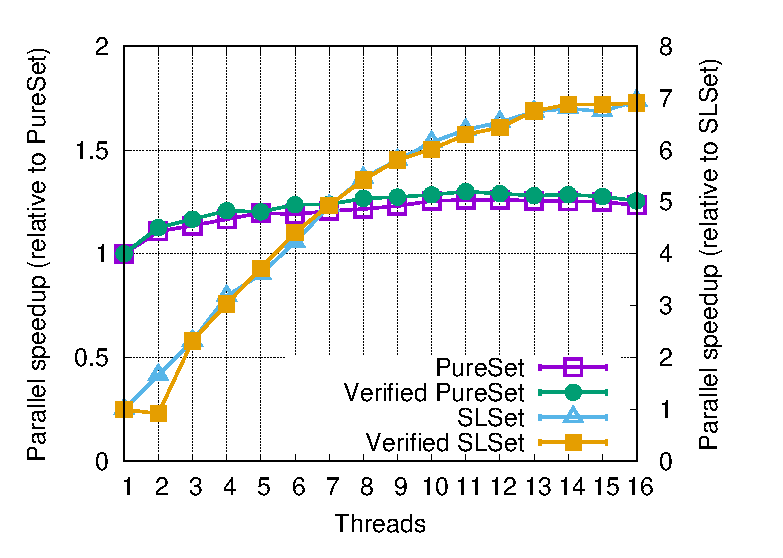
\includegraphics[width=3.2in]{text/refinementreflection/set.eps}
  \end{center}
  \caption{Parallel speedup for doing 1 million parallel inserts over 10
    iterations, verified and unverified, relative to the unverified version,
    for PureSet and SLSet.}
  \label{fig:set}
\end{figure}

\subsection{\texttt{monad-par}: $n$-body simulation}
\label{sec:nbody}
Next, we verify deterministic behavior of an
$n$-body simulation program that leverages @monad-par@, a Haskell library which
provides deterministic parallelism for pure code \cite{monad-par}.

Each simulated particle is represented by a
type @Body@ that stores its position, velocity and mass.
%
The function @accel@ computes the relative acceleration
between two bodies:
\begin{mcode}
  accel :: Body -> Body -> Accel
\end{mcode}
where @Accel@ represents the three-dimensional acceleration
\begin{mcode}
  data Accel = Accel Real Real Real
\end{mcode}
%
To compute the total acceleration
of a body @b@ we
(1) compute the relative acceleration between @b@
and each body of the system (@Vec Body@) and
(2) we add each acceleration component.
%
For efficiency, we use a parallel @mapReduce@ for the above
computation that
first \textit{maps} each vector body to get the acceleration relative to @b@
(@accel b@) and then adds each @Accel@ value by pointwise addition.
%
@mapReduce@ is only deterministic if the element is a @VerifiedMonoid@
from \S~\ref{sec:detpar}.
%%
%%To compute the velocity of each body in the simulation
%%we map reduce
%%
%%
%%An $n$-body simulation is used to model the behavior of particles in some system
%%in which forces are acting on the particles. The code which we verify is adapted
%%from an implementation of the all-pairs variant (a traditional, brute-force
%%approach) to $n$-body simulation from \cite{parallel-n-body}. The datatype which
%%we are verifying represents a particle:
%%
%%
\begin{mcode}
mapReduce :: VerifiedMonoid b 1=> (a1->b) 1-> Vec a 1-> b
\end{mcode}
%
To enforce the determinism of an $n$-body simulation, we need to provide a
@VerifiedMonoid@ instance for @Accel@.
%
We can easily prove that (@Real@, @+@, @0.0@)
is a monoid.
%
By product proof composition, we get a verified monoid instance for
\begin{mcode}
  type Accel' = (Real, (Real, Real))
\end{mcode}
which is isomorphic to @Accel@ (\ie @Iso Accel' Accel@).

Figure~\ref{fig:nbody} shows the results of running two versions of the $n$-body
simulation with 2,048 bodies over 5 iterations, with and without verification,
using floating point doubles for \texttt{Real}\footnote{Floating point numbers
  notoriously violate associativity, but we use this approximation because
  Haskell does net yet have an implementation of {\em
    superaccumulators}~\cite{superaccumulation}.}. Notably, the two programs have almost
identical runtime performance.  This demonstrates that even when verifying code
that is run in a tight loop (like @accel@), we can expect that our programs
will not be slowed down by an unacceptable amount.

\begin{figure}
  \begin{center}
    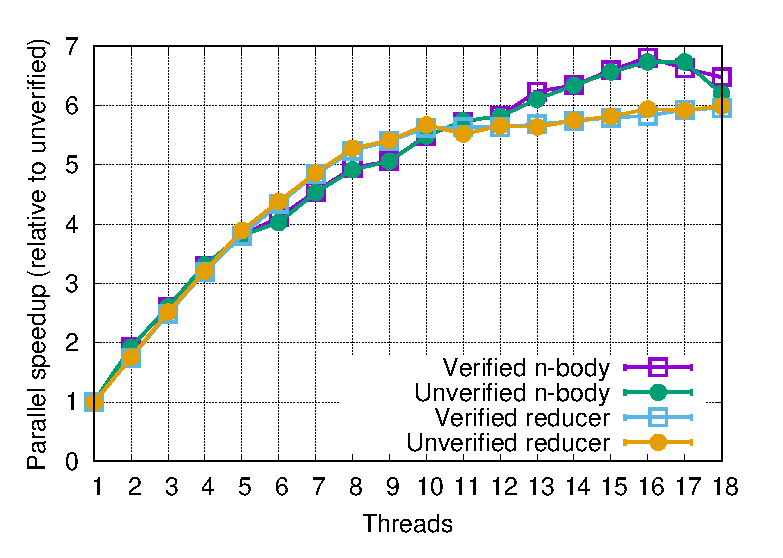
\includegraphics[width=3.2in]{text/refinementreflection/nbody.eps}
  \end{center}
  \caption{Parallel speedup for doing a parallel $n$-body simulation and
      parallel array reduction. The speedup is relative to the
    unverified version of each respective class of program.}
  \label{fig:nbody}
\end{figure}

\subsection{DPJ: Parallel Reducers}
\label{sec:reducer}
%% Our last benchmark illustrates how one can enforce various deterministic properties
%% that are different from the standard class properties (\ie monoid associativity).
%% For example,
The Deterministic Parallel Java (DPJ) project provides
a deterministic-by-default semantics for the Java programming language~\cite{DPJ}.
%
In DPJ, one can declare a method as @commutative@ and thus {\em assert} that
racing instances of that method result in a deterministic outcome.
For example:
%
% private region AccumRgn, static int sum in AccumRgn;
%% private static commutative synchronized
%%  void updateSum(int n) writes AccumRgn { sum += n; }
\begin{code}
commutative void updateSum(int n) writes R
  { sum += n; }
\end{code}
But, DPJ provides no means to formally prove commutativity and thus
determinism of parallel reduction.
In Liquid Haskell, we specified commutativity as an extra proof method
that extends the @VerifiedMonoid@ class.
%
\begin{mcode}
 class VerifiedMonoid a => VerifiedComMonoid a where
  commutes :: x:a -> y:a -> { x <> y = y <> x }
\end{mcode}
%
Provably commutative appends can be used to deterministically
update a reducer variable, since the result is the same regardless
of the order of appends.
%
We used LVish~\cite{kuper2014freeze} to
encode a reducer variable with a value @a@ and a region @s@
as @RVar s a@.
\begin{mcode}
 newtype RVar s a
\end{mcode}
We specify that safe (\ie deterministic)
parallel updates require provably commutative appending.
\begin{mcode}
  updateRVar :: VerifiedComMonoid a
             => a -> RVar s a -> Par s ()
\end{mcode}
%
Following the DPJ program, we used @updateRVar@'s provably deterministic interface
to compute, in parallel, the sum of an array with $3$x$10^9$ elements by updating
a single, global reduction variable using a varying number of threads.
%
Each thread sums segments of an array, sequentially, and updates the variable
with these partial sums.
%
In Figure \ref{fig:nbody}, we compare the verified and unverified versions
of our implementation to observe no appreciable
difference in performance.


\section{Conclusions \& Future Directions}

We have shown how refinement reflection -- namely
reflecting the definitions of functions in their
output refinements -- can be used to convert a
language into a proof assistant, while ensuring
(refinement) type checking stays decidable and
predictable via careful design of the logic and
proof combinators.

Our evaluation shows that refinement reflection
lets us prove deep specifications of a variety
of implementations, and identifies
important avenues for research.
%
First, while proofs are \emph{possible}, they can
sometimes be \emph{cumbersome}. For example, in
the proof of associativity of the monadic bind
operator for the @Reader@ monad three of eight
(extensional) equalities required explanations,
some nested under multiple $\lambda$-abstractions.
%
Thus, it would be valuable to use recent
advances in refinement-based synthesis~\cite{polikarpova16}
to automate proof construction.
%
Second, while our approach to $\alpha$- and
$\beta$-equivalence is sound, we do not know
if it is \emph{complete}. We conjecture it is,
due to the fact that our refinement terms
are from the simply typed lambda calculus (STLC).
%
Thus, it would be interesting to use the
normalization of STLC to develop a sound
and complete SMT axiomatization, thereby
automating proofs predictably.

%% We extended Liquid Types to allow reasoning about program functions.
%% %
%% We represent program functions into logic as uninterpreted functions
%% and
%% capture the behavior of functions in the result of the function's
%% types.
%% %
%% We preserved decidable type checking by requiring the user,
%% to explicitly invoke functions,
%% instead of the solver to instantiate functional axioms.
%%
%% In the future we plan to embed existing heuristics and tactics
%% from dependent type languages, like Coq and Adga,
%% to automate common proof procedures.


\mypara{Acknowledgments}
The material of this chapter have been submitted for publication as it may appear in PLDI 2017:
\noindent Vazou, Niki; Choudhury, Vikraman; Scott, Ryan G.; Newton, Ryan R.; Jhala, Ranjit.
``Refinement Reflection: Parallel Legacy Languages as Theorem Provers''.



\chapter{Case Study: Parallel String Matcher}\label{stringmatcher}

\makequote{The way the processor industry is going, is to add more and more cores,\\
but nobody knows how to program those things.}{Steve Jobs}

In this chapter,
we prove correctness of parallelization of a na\"ive string matcher
using Haskell as a theorem prover.
%
We use refinement types to specify correctness properties,
Haskell terms to express proofs 
-- via Refinement Reflection from chapter~\ref{refinementrflection}--
and \toolname to check correctness of proofs.

Optimization of sequential functions via parallelization
is a well studied technique~\cite{jaja,blelloch}.
%
Paper and pencil proofs have been developed to support the
correctness of the transformation~\cite{Cole93parallelprogramming}.
%
However, these paper written proofs
show correctness of the parallelization algorithm
and do not reason about the actual implementation
that may end up being buggy.

Dependent Type Systems (like Coq~\cite{coq-book} and Adga~\cite{agda} )
enable program equivalence proofs
for the actual implementation of the functions to be parallelized.
%
For example, SyDPaCC~\cite{SyDPaCC} is a Coq extension that
given a na\"ive Coq implementation of a function,
returns an Ocaml parallelized version with a proof of program equivalence.
%
The limitation of this approach is that the initial
function should be implemented in
the specific dependent type framework
and thus cannot use features and libraries from one's favorite
programming language.

In chapter~\ref{refinementrflection}
we claimed that Refinement Reflection can turn any programming
language into a proof assistant.
%
In this chapter we check our claim and use \toolname
to prove program equivalence.
%
Specifically,
we \textit{define in Haskell}
a sequential string matching function, @toSM@, and its parallelization, @toSMPar@,
using existing Haskell libraries; then,
we \textit{prove in Haskell} that these two functions are equivalent;
finally, we check our proofs using \toolname.

\mypara{Theorems as Refinement Types}
Refinement Types refine types with properties
drawn from decidable logics.
For example, the type @{v:Int | 0 < v}@
describes all integer values @v@ that are greater than @0@.
%
We refine the unit type to express theorems,
define unit value terms to express proofs, and use
\toolname to check that the proofs prove the theorems.
%
For example, \toolname accepts
the type assignment @() :: {v:()| 1+1=2}@,
as the underlying SMT can always prove the equality @1+1=2@.
%
We write @{1+1=2}@ to simplify the type @{v:()| 1+1=2}@
from the irrelevant binder @v:()@.

\mypara{Program Properties as Types}
The theorems we express can refer to program functions.
As an example, the type of @assoc@ expresses that @mappend@
is associative.
%
\begin{code}
  assoc :: x:m -> y:m -> z:m -> {x mappend (y mappend z) = (x mappend y) mappend z}
\end{code}
%
In \S~\ref{sec:haskell-proofs} we explain
how to write Haskell proof terms to prove theorems like @assoc@
by proving that list append @(++)@ is associative.
%
Moreover, we prove that the empty list @[]@ is the identity element of
list append and conclude that the list
(with @[]@ and @(++)@, \ie the triple (@[a]@, @[]@, @(++)@))
is provably a monoid.

\mypara{Corectness of Parallelization}
In \S~\ref{sec:parallelization}, we define the type @Morphism n m f@ that specifies
that @f@ is a \textit{morphism} between two monoids
(@n@, @$\eta$@, @<+>@) and (@m@, @$\epsilon$@, @<>@),
% \ie @f@ distributes among them or, equivalently, @f (x <+> y) = f x <> f y@.
\ie @f :: n -> m@ where @f $\eta$ = $\epsilon$@ and @f (x <+> y) = f x <> f y@.

A morphism @f@ on a ``chunkable'' input type can be parallelized by:
\begin{itemize}
  \item chunking up the input in @j@ chunks (@chunk j@),
  \item applying the morphism in parallel to all chunks (@pmap f@), and
  \item recombining the mapped chunks via @mappend@, also in parallel (@pmconcat i@).
\end{itemize}
%
We specify correctness of the above transformation as a refinement type.
%
\begin{code}
  parallelismEq
    :: f:(n -> m) -> Morphism n m f -> x:n -> i:Pos -> j:Pos
    -> {f x = pmconcat i (pmap f (chunk j x))}
\end{code}
%
\S~\ref{sec:parallelization} describes the parallelization transformation in details
concluding with 
Correctness of Parallelization Theorem~\ref{theorem:two-level} 
that proves correctness by a Haskell definition of @parallelismEq@ 
that satisfies the above type.

\mypara{Case Study: Parallelization of String Matching}
We use the above theorem to parallelize string matching.
We define a string matching function @toSM :: RString -> toSM target@
from a \textit{refined string} to a \textit{string matcher}.
%
A refined string (\S~\ref{subsec:refinedstrings}) is a wrapper around
the efficient string manipulation library
@ByteString@ that moreover assumes
various string properties, including the monoid laws.
%
A string matcher @SM target@ (\S~\ref{subsec:stringmatcher}) is a data type that contains
a refined string and a list of all the indices
where the type level symbol @target@ appears in the input.
%
We prove that @SM target@ is a monoid and @toSM@ is a morphism,
thus by the aforementioned Correctness of Parallelization Theorem~\ref{theorem:two-level}
we can correctly parallelize string matching.


To sum up, we present the first realistic proof that 
uses Haskell as a theorem prover:
correctness of parallelization on string matching.
%
This chapter is summarized as follows
\begin{itemize}
\item We explain how theorems and proofs are encoded and machine checked in \toolname
by formalizing monoids and proving that lists are monoids
(\S~\ref{sec:haskell-proofs}).
\item We formalize morphisms between monoids and
specify and prove correctness of parallelization of morphisms
(\S~\ref{sec:parallelization}).
\item We show how libraries can be imported as trusted components by wrapping
@ByteString@s as refined strings which satisfy the monoid laws (\S~\ref{subsec:refinedstrings}).
\item As an application, we prove that a string matcher is a morphism between the monoids of refined strings
and string matchers,  thus we get provably correct parallelization of string matching (\S~\ref{sec:stringmatching}).
\item Based on our approximately 2K lines of code proof we evaluate the approach of using Haskell as a theorem prover
(\S~\ref{sec:stringmatcher:evaluation}).
\end{itemize}

%% \NV{TO CHECL that in the logic we use = instead of ==}
%% \NV{TO CHECK that list type is L a}
\section{Proofs as Haskell Functions}\label{sec:haskell-proofs}

Refinement Reflection~\cite{reflection} is a technique
that lets you write Haskell functions that prove theorems
about other Haskell functions and have your proofs machine-checked
by Liquid Haskell~\cite{Vazou14}.
%
As an introduction to Refinement Reflection,
in this section, we prove that lists are monoids by
\begin{itemize}
\item \textit{specifying monoid laws} as refinement types,
\item \textit{proving the laws} by writing the implementation of the law specifications, and
\item \textit{verifying the proofs} using Liquid Haskell.
\end{itemize}

\subsection{Reflection of data types into logic.}
To start with,
we define a List data structure and
teach Liquid Haskell basic properties about List,
namely, how to check that proofs on lists are \textit{total}
and how to encode functions on List into the logic.

The data list definition @L@ is the standard recursive definition.
\begin{code}
data L [length] a = N | C a (L a)
\end{code}
%
With the @length@ annotation in the definition Liquid Haskell
will use the @length@ function to check termination
of functions recursive on Lists.
%
We define @length@ as the standard Haskell function
that returns natural numbers.
%
We lift @length@ into logic as a \textit{measure}~\cite{Vazou14},
that is, a \textit{unary} function whose (1) domain is the data type, and
(2) body is a single case-expression over the datatype.
\begin{code}
type Nat = {v:Int | 0 <= v}

measure length
length         :: L a -> Nat
length N        = 0
length (C x xs) = 1 + length xs
\end{code}

Finally, we teach Liquid Haskell how to encode functions on Lists
into logic.
%
The flag @"--exact-data-cons"@
automatically derives measures which
(1) test if a value has a given data constructor, and
(2) extract the corresponding field's value.
%
For example, Liquid Haskell will automatically derive the following
List manipulation measures from the List definition.
\begin{code}
isN :: L a -> Bool    -- Haskell's null
isC :: L a -> Bool    -- Haskell's not . null

selC1 :: L a -> a     -- Haskell's head
selC2 :: L a -> L a   -- Haskell's tail
\end{code}
%
Next, we describe how Liquid Haskell uses the above measures
to automatically reflect Haskell functions on Lists into logic.

\subsection{Reflection of Haskell functions into logic.}
Next, we define and reflect into logic the two monoid operators on Lists.
Namely, the identity element @mempty@ (which is the empty list)
and an associative operator @(mappend)@ (which is list append).
%
\begin{code}
reflect mempty
mempty :: L a
mempty = N

reflect (mappend)
(mappend) :: L a -> L a -> L a
N        mappend ys = ys
(C x xs) mappend ys = C x (xs mappend ys)
\end{code}

The reflect annotations lift the Haskell functions into logic in three steps.
%
First, check that the Haskell functions indeed terminate by checking
that the @length@ of the input list is decreasing,
as specified in the data list definition.
%
Second, in the logic, they define the respective uninterpreted functions
@mempty@ and @(mappend)@.
%
Finally, the Haskell functions and the logical uninterpreted functions
are related by strengthening the result type of the Haskell function
with the definition of the function's implementation.
%
For example, with the above @reflect@ annotations,
Liquid Haskell will \textit{automatically} derive the following strengthened
types for the relevant functions.
\begin{code}
mempty  :: {v:L a | v = mempty && v = N }

(mappend):: xs:L a -> ys:L a
    ->  {v:L a | v = xs mappend ys
              && v = if isN xs then ys
                     else C (selC1 xs) (selC2 xs mappend ys)
        }
\end{code}

\subsection{Specification and Verification of Monoid Laws}

Now we are ready to specify the monoid laws as refinement types and
provide their respective proofs as terms of those type. Liquid Haskell
will verify that our proofs are valid. 
%
Note that this is exactly what
one would do in any standard logical framework,
like LF~\cite{Harper93}.

The type @Proof@ is defined as an alias of the unit type (@()@)
in the library @ProofCombinators@ that comes with Liquid Haskell.
Figure~\ref{figure:proofcombinators} summarizes the definitions we use from @ProofCombinators@.
%
We express theorems as refinement types by refining
the @Proof@ type with appropriate refinements.
%
For example, the following theorem states
the @mempty@ is always equal to itself.
\begin{code}
trivial :: {mempty = mempty}
\end{code}
%
Where @{mempty = mempty}@ is a simplification for the @Proof@ type
@{v:Proof | mempty = mempty}@, since the binder @v@ is irrelevant, and
@trivial@ is defined in @ProofCombinators@ to be unit.
%
Liquid Haskell will typecheck the above code using an SMT
solver to check congruence on @mempty@.
%% \NV congruence on or with?
%

\begin{definition}[Monoid] \label{definition:monoid}
The triple (@m@, @epsilon@, @<>@) is a monoid
(with identity element @epsilon@ and associative operator @<>@),
if the following functions are defined. % on @m@.
%
\begin{code}
idLeft_m :: x:m -> {mempty mappend x = x}
idRight_m :: x:m -> {x mappend mempty = x}
assoc_m :: x:m -> y:m -> z:m -> {x mappend (y mappend z) = (x mappend y) mappend z}
\end{code}
\end{definition}
%
Using the above definition, we prove that our list type @L@ is a monoid
by defining Haskell proof terms that satisfy the above monoid laws. 
%%We now represent these conditions applied to our list type @L@ and
%%their proofs as (refined) types and terms of those types.

\paragraph{Left Identity} is expressed
as a refinement type signature that takes as input
a list @x:L a@ and returns a @Proof@ type refined
with the property @mempty <> x = x@
\begin{code}
idLeft :: x:L a -> { mempty mappend x = x }
idLeft x = empty <> x ==. N <> x ==. x *** QED
\end{code}
%
We prove left identity using combinators from @ProofCombinators@ as
defined in Figure~\ref{figure:proofcombinators}.
%
We start from the left hand side @empty <> x@,
which is equal to @N <> x@ by calling @empty@ thus
unfolding the equality @empty = N@ into the logic.
%
Next, the call @N <> x@ unfolds into the logic the definition of @(<>)@
on @N@ and @x@, which is equal to @x@, concluding our proof.
%
Finally, we use the operators @p *** QED@ which basically casts @p@ into a proof term.
%
In short, the proof of left identity, proceeds by unfolding the definitions of @mempty@
and @(<>)@ on the empty list.

\begin{figure}[t]
\begin{code}
type Proof = ()
data QED   = QED

trivial :: Proof
trivial = ()

(==.) :: x:a -> y:{a | x = y} -> {v:a | v = x}
x ==. _ = x

(***) :: a -> QED -> Proof
_ *** _ = ()

(?) :: (Proof -> a) -> Proof -> a
f ? y = f y
\end{code}
\caption{Operators and Types defined in \texttt{ProofCombinators}}
\label{figure:proofcombinators}
\end{figure}

\paragraph{Right identity} is proved by structural induction.
%
We encode inductive proofs by case splitting on the base and inductive case,
and enforcing the inductive hypothesis via a recursive call.
\begin{code}
idRight :: x:L a -> { x <> mempty = x }
idRight N = N <> empty ==. N *** QED

idRight (C x xs)
   =   (C x xs) <> empty
   ==. C x (xs <> empty)
   ==. C x xs ? idRight xs
   *** QED
\end{code}
The recursive call @idRight xs@ is provided
as a third optional argument in the @(==.)@
operator to justify the equality @xs <> empty = xs@,
while the operator @(?)@ is merely a function application
with the appropriate precedence.
%
Note that LiquiHaskell, via termination and totality checking,
is verifying that all the proof terms are well formed because
(1) the inductive hypothesis is only applying to smaller terms, and
(2) all cases are covered.


\paragraph{Associativity} is proved in a very similar manner,
using structural induction.
%
\begin{code}
assoc   :: x:L a -> y:L a -> z:L a
        -> { x mappend (y mappend z) = (x mappend y) mappend z}
assoc N y z
  =   N <> (y <> z)
  ==. y <> z
  ==. (N <> y) <> z
  *** QED

assoc (C x xs) y z
  =  (C x xs) <> (y <> z)
  ==. C x (xs <> (y <> z))
  ==. C x ((xs <> y) <> z) ? associativity xs y z
  ==. (C x (xs <> y)) <> z
  ==. ((C x xs) <> y) <> z
  *** QED
 \end{code}
%
As with the left identity, the proof proceeds by
(1) function unfolding (or rewriting in paper and pencil proof terms),
(2) case splitting (or case analysis), and
(3) recursion (or induction).

Since our list implementation satisfies the three monoid laws
we can conclude that @L a@ is a monoid.
%

%% \NV{I need to discuss the difference between representation of proof terms and methods in the logic}

\begin{theorem}\label{theorem:monoid:list}
(@L a@, @epsilon@, @<>@) is a monoid.
\end{theorem}
\begin{proof}
@L a@ is a monoid, as the implementation of
@idLeft@, @idRight@, and @assoc@
satisfy the specifications of
@idLeft_m@, @idRight_m@, and @assoc_m@, with @m = L a@.
\qed\end{proof}

\section{Verified Parallelization of Monoid Morphisms}\label{sec:parallelization}

A monoid morphism is a function between two monoids which
preserves the monoidal structure; \ie a function on the underlying
sets which preserves identity and associativity. We formally specify
this definition using a refinement type @Morphism@.
%
\begin{definition}[Monoid Morphism]\label{definition:morphism}
A function @f :: n -> m@ is a morphism
between the monoids
(@m@, @$\epsilon$@, @<>@)
and (@n@, @$\eta$@, @<+>@)
if @Morphism n m f@ has an inhabitant.
\begin{code}
type Morphism n m F =
  x:n -> y:n -> {F eta = epsilon && F (x <+> y) = F x <> F y}
\end{code}
\end{definition}

A monoid morphism can be parallelized when its domain can be cut into
chunks and put back together again, a property we refer to as
chunkable and expand upon in \S~\ref{subsec:chunkable}. A
chunkable monoid morphism is then parallelized by:
\begin{enumerate}
  \item chunking up the input,
  \item applying the morphism in parallel to all chunks, and
  \item recombining the chunks, also in parallel, back to a single value.
\end{enumerate}
In the rest of this section we implement and verify to be correct the above
transformation.

\subsection{Chunkable Monoids}\label{subsec:chunkable}
\begin{definition}[Chunkable Monoids]\label{definition:chunkable}
A monoid (@m@, @epsilon@, @<>@) is chunkable
if the following four functions are defined on @m@.
\begin{code}
length_m :: m -> Nat

drop_m :: i:Nat -> x:MGEq m i -> MEq m (length_m x-i)
take_m :: i:Nat -> x:MGEq m i -> MEq m i

takeDropProp_m :: i:Nat -> x:m ->
                  {x = take_m i x <> drop_m i x}
\end{code}

Where the type aliases @MLeq m I@ (and @MEq m I@)
constrain the monoid @m@ to have @length_m@
greater than (resp. equal) to @I@.
\begin{code}
type MGEq m I = {x:m | I <= length_m x }
type MEq  m I = {x:m | I = length_m x }
\end{code}
\end{definition}

Note that the ``important'' methods of chunkable monoids
are the @take@ and @drop@, while the @length@ method is required
to give pre- and post-condition on the other operations.
%
Finally, @takeDropProp@ provides a proof that
for each @i@ and monoid @x@, appending
@take i x@ to @drop i x@ will reconstruct @x@.

Using @take_m@ and @drop_m@ we define for each chunkable monoid
(@m@, @epsilon@, @<>@) a function @chunk_m i x@ that
splits @x@ in chunks of size @i@.
\begin{code}
chunk_m :: i:Pos -> x:m -> {v:L m | chunkRes_m i x v }
chunk_m i x
  | length_m x <= i = C x N
  | otherwise     = take_m i x `C` chunk_m i (drop_m i x)

chunkRes_m i x v
  | length_m x <= i = length_m v == 1
  | i == 1        = length_m v == length_m xs
  | otherwise     = length_m v < length_m xs
\end{code}

%
The function @chunk_m@ provably terminates as
@drop_m i x@
will return a monoid smaller than @x@,
by the Definition of @drop_m@.
%
The definitions of both @take_m@ and @drop_m@
are also used from Liquid Haskell to verify the
@length_m@ constraints in the result of @chunk_m@.

\ignore{
As a concrete example, to define list chunking, we first define the @take@ and @drop@
methods on the list monoid of section~\ref{sec:haskell-proofs}.
%
\begin{code}
take i N                    = N
take i (C x xs) | i == 0    = N
                | otherwise = C x (take (i-1) xs)

drop i N                    = N
drop i (C x xs) | i == 0    = C x xs
                | otherwise = drop (i-1) xs
\end{code}
We can prove that the above definitions
combined with the @length@ of section~\ref{sec:haskell-proofs}
satisfy the specifications
of the Chunkable Monoid Definition~\ref{definition:chunkable}.
%
Thus, we can prove that the aforementioned list data type,
extended with the appropriate implementation for @takeDropProp@
is a chunkable monoid.
}

\subsection{Parallel Map}
We define a parallelized map function @pmap@
using Haskell's library @parallel@.
%
Concretely, we use the function
@Control.Parallel.Strategies.withStrategy@
that computes its argument in parallel given a parallel strategy.
\begin{code}
pmap :: (a -> b) -> L a -> L b
pmap f xs = withStrategy parStrategy (map f xs)
\end{code}
%
The strategy @parStrategy@ does not affect verification.
%
In our codebase we choose the traversable strategy.
\begin{code}
parStrategy :: Strategy (L a)
parStrategy = parTraversable rseq
\end{code}

\paragraph{Parallelism in the Logic.}
The function @withStrategy@ is an imported Haskell library function,
whose implementation is not available during verification.
%
To use it in our verified code, we make the \textit{assumption}
that it always returns its second argument.
\begin{code}
assume withStrategy :: Strategy a -> x:a -> {v:a | v = x}
\end{code}
%
Moreover, we need to reflect the function @pmap@ and represent its
implementation in the logic.
%
Thus, we also need to represent the function @withStrategy@ in the logic.
%
LiquidHaskell represents @withStrategy@ in the logic as a logical
function that merely returns
its second argument, @withStrategy _ x = x@,
and does not reason about parallelism.


\subsection{Monoidal Concatenation}\label{subsec:mconcat}
The function @chunk_m@ lets us turn a monoidal value into several
pieces. In the other direction, for any monoid @m@, there is a
standard way of turning @L m@ back into a single @m@~\footnote{\texttt{mconcat} is usually defined as \texttt{foldr mappend mempty}}
\begin{code}
  mconcat :: L m -> m
  mconcat N        = mempty
  mconcat (C x xs) = x <> mconcat xs
\end{code}
%
For any chunkable monoid @n@,
%
monoid morphism @f :: n -> m@,
%
and natural number @i > 0@
%
we can write a chunked version of @f@ as
\begin{code}
  mconcat . pmap f . chunk_n i :: n -> m.
\end{code}
Before parallelizing @mconcat@, we will prove that the previous function is equivalent to @f@.

\begin{theorem}[Morphism Distribution]\label{theorem:monoid:distribution}
Let (@m@, @$\epsilon$@, @<>@) be a monoid
and (@n@, @$\eta$@, @<+>@) be a chunkable monoid.
%
Then, for every morphism @f :: n -> m@,
every positive number @i@ and input @x@,
@f x = mconcat (pmap f (chunk_n i x))@ holds.
%
\begin{code}
morphismDistribution
  :: f:(n -> m) -> Morphism n m f -> x:n -> i:Pos
  -> {f x = mconcat (pmap f (chunk_n i x))}
\end{code}
\end{theorem}

\begin{proof}
We prove the theorem by providing an implementation of
@morphismDistribution@ that satisfies its type.
%
The proof proceeds by induction on the length of the input.
%
\begin{code}
morphismDistribution f thm x i
  | length_n x <= i
  =   mconcat (pmap f (chunk_n i x))
  ==. mconcat (map f (chunk_n i x))
  ==. mconcat (map f (C x N))
  ==. mconcat (f x `C` map f N)
  ==. f is <> mconcat N
  ==. f is <> epsilon
  ==. f is ? idRight_m (f is)
  *** QED
morphismDistribution f thm x i
  =   mconcat (pmap f (chunk_n i x))
  ==. mconcat (map f (chunk_n i x))
  ==. mconcat (map f (C takeX) (chunk_n i dropX)))
  ==. mconcat (f takeX `C` map f (chunk_n n dropX))
  ==. f takeX <> f dropX
      ? morphismDistribution f thm dropX i
  ==. f (takeX <+> dropX)
      ? thm takeX dropX
  ==. f x
      ? takeDropProp_n i x
  *** QED
  where
    dropX = drop_n i x
    takeX = take_n i x
\end{code}
%
In the base case we use rewriting and right identity on the monoid @f x@.
%
In the inductive case,
we use the inductive hypothesis on the input @dropX = drop_n i x@,
that is provably smaller than @x@ as @1 < i@.
%
Then, the fact that @f@ is a monoid morphism,
as encoded by our assumption argument @thm takeX dropX@
we get basic distribution of @f@, that is
@f takeX <> f dropX = f (takeX <+> dropX)@.
%
Finally, we merge @takeX <+> dropX@ to @x@
using the property @takeDropProp_n@ of the chunkable monoid @n@.
\qed\end{proof}


\subsection{Parallel Monoidal Concatenation}\label{subsec:pmconcat}
%
We now parallelize the monoid concatenation by defining a
@pmconat i x@ function that chunks the input list of monoids and concatenates each
chunk in parallel.

We use the @chunk@ function of \S~\ref{subsec:chunkable} instantiated to @L m@ to define a parallelized version of
monoid concatenation @pmconcat@.
\begin{code}
pmconcat :: Int -> L m -> m
pmconcat i x | i <= 1 || length x <= i
  = mconcat x
pmconcat i x
  = pmconcat i (pmap mconcat (chunk i x))
\end{code}
The function @pmconcat i x@ calls @mconcat x@ in the base case,
otherwise it
(1) chunks the list @x@ in lists of size @i@,
(2) runs in parallel @mconcat@ to each chunk,
(3) recursively runs itself with the resulting list.
%
Termination of @pmconcat@ holds, as the length of @chunk i x@
is smaller than the length of @x@, when @1 < i@.

Next, we prove equivalence of parallelized monoid concatenation.
%
\begin{theorem}[Correctness of Parallelization]\label{theorem:equivalence:concat}
Let (@m@, @$\epsilon$@, @<>@) be a monoid.
Then, the parallel and sequential concatenations are equivalent.
\begin{code}
pmconcatEquivalence
  :: i:Int -> x:L m -> { pmconcat i x = mconcat x }
\end{code}
\end{theorem}

\begin{proof}
We prove the theorem by providing a Haskell implementation of @pmconcatEquivalence@
that satisfies its type.
%
The details of the proof can be found in~\cite{implementation},
here we provide the sketch of the proof.

First, we prove that @mconcat@ distributes over list splitting
\begin{code}
mconcatSplit
  :: i:Nat -> xs:{L m | i <= length xs}
  -> { mconcat xs = mconcat (take i xs)
                 <> mconcat (drop i xs) }
\end{code}
%
The proofs proceeds by structural induction, using monoid left identity in the base case
and monoid associativity associavity and unfolding of @take@ and @drop@
methods in the inductive step.

We generalize the above lemma
to prove that @mconcat@ distributes over list chunking.
\begin{code}
mconcatChunk
  :: i:Pos -> xs:L m
  -> { mconcat xs = mconcat (map mconcat (chunk i xs)) }
\end{code}
%
The proofs proceeds by structural induction, using monoid left identity in the base case
and lemma @mconcatSplit@ in the inductive step.

Lemma @mconcatChunk@ is sufficient to prove @pmconcatEquivalence@ by structural induction,
using monoid left identity in the base case.
\qed\end{proof}

\subsection{Parallel Monoid Morphism}\label{subsec:both-levels}
We can now replace the @mconcat@ in our chunked monoid morphism in
\S~\ref{subsec:mconcat} with @pmconcat@ from
\S~\ref{subsec:pmconcat} to provide an implementation that uses
parallelism to both map the monoid morphism and concatenate the
results.

%\paragraph{Correctness} of our parallel monoid morphism follows from Theorems~\ref{theorem:monoid:distribution} and~\ref{theorem:equivalence:concat}.
%
\begin{theorem}[Correctness of Parallelization]\label{theorem:two-level}
Let (@m@, @$\epsilon$@, @<>@) be a monoid
and (@n@, @$\eta$@, @<+>@) be a chunkable monoid.
%
Then, for every morphism @f :: n -> m@,
every positive numbers @i@ and @j@, and input @x@,
@f x = pmconcat i (pmap f (chunk_n j x))@ holds.
%
\begin{code}
parallelismEquivalence
  :: f:(n -> m) -> Morphism n m f -> x:n -> i:Pos -> j:Pos
  -> {f x = pmconcat i (pmap f (chunk_n j x))}
\end{code}
\end{theorem}

\begin{proof}
We prove the theorem by providing an implementation of
@parallelismEquivalence@ that satisfies its type.
%
\begin{code}
parallelismEquivalence f thm x i j
  =   pmconcat i (pmap f (chunk_n j x))
  ==. mconcat (pmap f (chunk_n j x))
      ? pmconcatEquivalence i (pmap f (chunk_n j x))
  ==. f x
      ? morphismDistribution f thm x j
  *** QED
\end{code}
The proof follows merely by application of the 
two previous Theorems~\ref{theorem:monoid:distribution} and~\ref{theorem:equivalence:concat}.
\qed\end{proof}


\ignore{
\paragraph{A Basic Time Complexity} analysis of the algorithm
reveals that parallelization of morphism  leads to runtime speedups
on monads with fast (constant time) appending operator.

We want to compare the complexities of the sequential @f i@
and the two-level parallel @pmconcat i (pmap f (chunk_n j x))@.
%
Let $n$ be the size on the input @x@.
Then, the sequential version runs in time
$T_f(n) = O(n)$, that is equal to the time complexity of the morphism @f@ on input @i@.
%

The parallel version runs @f@ on inputs of size $n' = \frac{n}{j}$.
%
Assuming the complexity of @x <> y@ to be $T_\mappend(\text{max}(|\tx|, |\ty|))$,
complexity of @mconcat xs@ is $O((\texttt{length \txs}-1) T_\mappend(\text{max}_{\tx_i \in \txs}(|\tx_i|)))$.
%
Now, parallel concatenation, @pmconcat i xs@ at each iteration runs @mappend@
on a list of size @i@. Moreover,
at each iteration, divides the input list in chunks of size @i@, leading to
$\frac{\log|xs|}{\log i}$ iterations, and time complexity
$(i-1)(\frac{\log|xs|}{\log i})(T_\mappend(m))$
for some $m$ that bounds the size of the monoids.

The time complexity of parallel algorithm consists on the base cost on running @f@
at each chunk and then parallel concatenating the $\frac{n}{j}$ chunks.
\begin{equation}
O((i-1)(\frac{\log n - \log j}{\log i})T_\mappend(m) + T_f(\frac{n}{j})) \label{eq:complexity}
\end{equation}
%
Since time complexity depends on the time complexity of @<>@
for the parallel algorithm to be efficient time complexity of @<>@ should be constant.
%
Otherwise, if it depends on the size of the input, the size of monoids can grow at each iteration of @mconcat@.
%

Moreover, from the complexity analysis we observe that time grows on bigger @i@ and smaller @j@.
%
Thus, chunking the input in small chunks while splitting the monoid list in half leads
to more parallelism, and thus (assuming infinite processors and no caching) greatest speedup.
}

\section{Case Study: Correctness of Parallel String Matching}\label{sec:stringmatching}

\S~\ref{sec:parallelization} showed that any monoid morphism
whose domain is chunkable can be parallelized. We now make use of that
result to parallelize string matching. We start by observing that
strings are a chunkable monoid. %\NV add monoid methods
We then turn string matching for a
given target into a monoid morphism from a string to a suitable
monoid, @SM target@, defined in
\S~\ref{subsec:stringmatcher}. 
Finally, in \S~\ref{subsec:parallel-string-matching}, we parallelize string matching
by a simple use of the
parallel morphism function of \S~\ref{subsec:both-levels}. 

\ignore{
  In this section we apply the Correctness of Parallelization Theorem~\ref{theorem:two-level}
to a string matching function @toSM@
that is a morphism between strings and the indices where a target string appears,
to get correctness of parallelization of @toSM@.

We define @toSM :: RString -> SM target@
from a Refined String data type @RString@
to a dependently typed string maching data type @SM target@
where @target@ represents the substring to be matched.
%
To apply Theorem~\ref{theorem:two-level} on @toSM@ we need to discharge three proof obligations.
%
\begin{itemize}
\item @RString@ is a chunkable monoid (\S~\ref{subsec:refinedstrings}),
\item @SM target@ is a monoid (\S~\ref{subsec:stringmatcher}), and
\item @toSM@ is a morphism between @RString@ and @SM target@ (\S~\ref{subsec:smmorphism}).
\end{itemize}
%
With these proof obligations discharged we conclude (\S~\ref{subsec:parallel-string-matching})
correctness of parallel string matching.
}

\subsection{Refined Strings are Chunkable Monoids}\label{subsec:refinedstrings}
We define a new type @RString@, which is a chunkable monoid, to be the
domain of our string matching function. Our type simply wraps
Haskell's existing @ByteString@.
\begin{code}
data RString = RS BS.ByteString
\end{code}
Similarly, we wrap the existing @ByteString@ functions we will need to
show @RString@ is a chunkable monoid.
\begin{code}
stringMempty = RS (BS.empty)
(RS x) stringMappend (RS y)= S (x `BS.append` y)

lenStr    (RS x) = BS.length x
takeStr i (RS x) = RS (BS.take i x)
dropStr i (RS x) = RS (BS.take i x)
\end{code}
Although it is possible to explicitly prove that @ByteString@
implements a chunkable monoid~\cite{realworldliquid14}, it is time
consuming and orthogonal to our purpose. Instead, we
just \textit{assume} the chunkable monoid properties of @RString@--
thus demonstrating that refinement reflection is capable of doing
gradual verification.


\ignore{
We follow the easy route, defining the @RString@ data type to be a wrapper of the
optimized @ByteString@ and

%
This allows our implementation to \textit{use the optimized library
functions} of @ByteString@; additionally, it shows that refinement
reflection can be used for \textit{gradual verification} where
verified code uses untrusted components that are explicitely assumed
to satisfy required properties.
%
Proving that @ByteString@ implements a chunkable monoid is feasible,
as evidenced by the current verification of Bytestring functions~\cite{realworldliquid14},
but it is time consuming and orthogonal to the string matching proof.
%
%% NV I need to automate this in LiquidHaskell!

We need to use the above operators to specify the chunkable monoid
laws, but we cannot reflect the operators in the logic, as the
ByteString functions do not exist in the logic.  We ``manually
reflect'' each of the above functions in the logic, by 1. defining a
logical uninterpreted function for each of them that assumed to be
equal to the Haskell functions and 2. use the logical functions to
specify the chunkable monoid laws.
}

For instance, we define a logical uninterpreted function
@stringMappend@ and relate it to the Haskell @stringMappend@ function
via an assumed (unchecked) type.
%
\begin{code}
assume (stringMappend)
  :: x:RString -> y:RString -> {v:RString | v = x stringMappend y}
\end{code}
%
Then, we use the uninterpreted function @stringMappend@ in the logic
to assume monoid laws, like associativity.
%
\begin{code}
assume assocStr :: x:RString -> y:RString -> z:RString
                 -> { x <+> (y <+> z) = (x <+> y) <+> z }
assocStr _ _     = trivial
\end{code}
%
Haskell applications of @stringMappend@ are interpreted in the logic
via the logical @stringMappend@ that satisfies associativity via theorem @assocStr@.

Similarly for the chunkable methods, we define the uninterpreted functions
@takeStr@, @dropStr@ and @lenStr@ in the logic,
and use them to strengthen the result types of the respective functions.
%
\ignore{
For example the type of @takeStr@ includes both the length specifications
from chunkable monoid and the uninterpreted function equality @v = takStr i x@.
\begin{code}
assume takeStr
  :: i:Nat -> x:{RString | i <= lenStr x}
  ->  {v:RString | lenStr v = i && v = takeStr i x }
\end{code}
We use the uninterpreted function @takeStr@ and @dropStr@ to
specify and \textit{assume} the @take@-@drop@ property of chunkable monoids.
\begin{code}
assume takeDropPropStr
 :: i:Nat -> x:RString -> {x = takeStr i x <+> dropStr i x}
takeDropPropStr _ _ = trivial
\end{code}
%
} With the above function definitions (in both Haskell and logic) and
assumed type specifications, Liquid Haskell will check (or rather
assume) that the specifications of chunkable monoid, as defined in the
Definitions~\ref{definition:monoid} and~\ref{definition:chunkable},
are satisfied.
%
We conclude with the assumption (rather that theorem)
that @RString@ is a chunkable monoid.
\begin{assumption}[RString is a Chunkable Monoid]\label{assumption:rstring}
(@RString@, @stringMempty@, @stringMappend@)
combined with the methods
@lenStr@, @takeStr@, @dropStr@ and @takeDropPropStr@
is a chunkable monoid.
\end{assumption}


\subsection{String Matching Monoid}\label{subsec:stringmatcher}
String matching is determining all the indices in a source string
where a given target string begins; for example, for source string
\texttt{ababab} and target \texttt{aba} the results of string
matching would be \texttt{[0, 2]}. 

We now define a suitable monoid, @SM target@, for the codomain of
a string matching function, where @target@ is the string being looked
for.
%
Additionally, we will define a function @toSM :: RString -> SM target@
which does the string matching and is indeed a monoid morphism from
@RString@ to @SM target@ for a given @target@.

\subsubsection{String Matching Monoid}

We define the data type
@SM target@ to contain a refined string field @input@ and
a list of all the indices in @input@ where the
@target@ appears.
%
\begin{code}
  data SM (target :: Symbol) where
    SM :: input:RString
       -> indices:[GoodIndex input target]
       -> SM target
\end{code}
%
We use the string type literal~\footnote{\texttt{Symbol} is a kind and
target is effectively a singleton type.} to parameterize the monoid
over the target being matched. This encoding allows the type checker
to statically ensure that only searches for the same target can be
merged together.  The input field is a refined string, and the indices
field is a list of good indices.  For simplicity we present lists as
Haskell's built-in lists, but our implementation uses the reflected
list type, @L@, defined in \S~\ref{sec:haskell-proofs}.

A @GoodIndex input target@ is a refined type alias for a natural
number @i@ for which @target@ appears at position @i@ of @input@.  As
an example, the good indices of @"abcab"@ on @"ababcabcab"@ are
@[2,5]@.
%
\begin{code}
  type GoodIndex Input Target
    = {i:Nat | isGoodIndex Input (fromString Target) i }

  isGoodIndex :: RString -> RString -> Int -> Bool
  isGoodIndex input target i
    = (subString i (lenStr target) input  == target)
    && (i + lenStr target <= lenStr input)

  subString :: Int -> Int -> RString -> RString
  subString o l = takeStr l . dropStr o
\end{code}
%
\ignore{
\begin{code}
goodSM :: SM "abcab"
goodSM = SM "ababcabcab" [2, 5]

badSM  :: SM "abcab"
badSM  = SM "ababcabcab" [0, 7]
\end{code}
\ignore{
\NV{Liquid Haskell actually will reject both the above, as the lenStr and subString functions are uninterpreted}
}
}

\subsubsection{Monoid Methods for String Matching}~\label{subsec:monoid:methods}
Next, we define the mappend and identity elements for string matching.

The \textit{identity element} @mempty@ of @SM t@, for each target @t@, is
defined to contain the identity @RString@ (@stringMempty@) and the
identity @List@ (@listMempty@).
\begin{code}
  mempty:: forall (t :: Symbol). SM t
  mempty = SM stringMempty listMempty
\end{code}
%

\ignore{
The associative operator, @(mappend)@,
appends the two input strings.
The appended indices, as depicted in Figure~\ref{fig:mappend:indices},
are the concatenations of three list indices:
\begin{enumerate}
\item The indices @xis@ of the first input, casted to good indices in the new structure,
\item the new indices @xyis@ created when concatenating the two strings, and
\item the indices @yis@ of the second input, shifted right @lenStr y@ units.
\end{enumerate}
%
}

\begin{figure}[t]
\centering
\captionsetup{justification=centering}
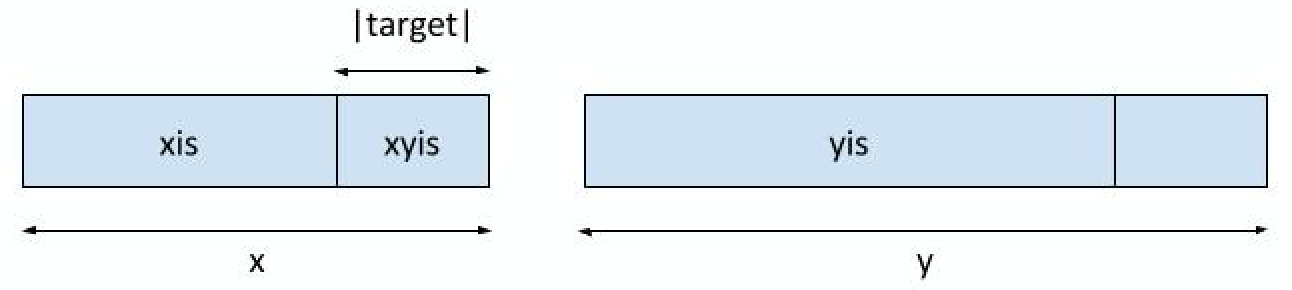
\includegraphics[scale=0.5]{text/stringmatcher/makeIndices}
\caption{Mappend indices of String Matcher.}
\label{fig:mappend:indices}
\end{figure}
%
The Haskell definition of @<>@, the monoid operation for @SM t@, is as follows.
\begin{code}
  (mappend)::forall (t::Symbol). KnownSymbol t => SM t -> SM t -> SM t
  (SM x xis) mappend (SM y yis)
    = SM (x stringMappend y) (xis' listMappend xyis listMappend yis')
    where
      tg   = fromString (symbolVal (Proxy :: Proxy t))
      xis' = map (castGoodIndexLeft tg x y) xis
      xyis = makeNewIndices x y tg
      yis' = map (shiftStringRight tg x y) yis
\end{code}
Note again that capturing target as a type parameter is critical,
otherwise there is no way for the Haskell's type system to specify
that both arguments of @(mappend)@ are string matchers on the same target.

The action of @(<>)@ on the two @input@ fields is straightforward;
however, the action on the two @indices@ is complicated by the need to
shift indices and the possibility of new matches arising from the
concatenation of the two @input@
fields. Figure~\ref{fig:mappend:indices} illustrates the three pieces
of the new @indices@ field which we now explain in more detail.

\mypara{1. Casting Good Indices}
If @xis@ is a list of good indices for the string @x@ and the target
@tg@, then @xis@ is also a list of good indices for the string
@x stringMappend y@ and the target @tg@, for each @y@.
%
To prove this property we need to invoke the property
@subStrAppendRight@ on Refined Strings that establishes
substring preservation on string right appending.
%
\begin{code}
  assume subStrAppendRight
      :: sl:RString -> sr:RString -> j:Int
      -> i:{Int | i + j <= lenStr sl }
      -> {subString sl i j = subString (sl stringMappend sr) i j}
\end{code}
%
The specification of @subStrAppendRight@ ensures that for each
string @sl@ and @sr@ and each integer @i@ and @j@ whose sum is within @sl@,
the substring from @i@ with length @j@ is identical in @sl@ and in @(sl stringMappend sr)@.
%
The function @castGoodIndexLeft@ applies the above property to an index @i@
to cast it from a good index on @sl@ to a good index on @(sl stringMappend sr)@
%
\begin{code}
  castGoodIndexLeft
    :: tg:RString -> sl:RString -> sr:RString
    -> i:GoodIndex sl tg
    -> {v:GoodIndex (sl stringMappend sr) target | v = i}

  castGoodIndexLeft tg sl sr i
    = cast (subStrAppendRight sl sr (lenStr tg) i) i
\end{code}
%
Where @cast p x@ returns @x@, after enforcing the properties of @p@ in the logic
\begin{code}
  cast :: b -> x:a -> {v:a | v = x}
  cast _ x = x
\end{code}
%
Moreover, in the logic, each expression @cast p x@
is reflected as @x@,
thus allowing random (\ie non-reflected) Haskell expressions to appear in @p@.

\mypara{2. Creation of new indices}
The concatenation of two input strings @sl@ and @sr@
may create new good indices.
%
For instance, concatenation of
@"ababcab"@ with @"cab"@
leads to a new occurence of @"abcab"@ at index @5@ which
does not occur in either of the two input strings.
%
These new good indices can appear only at the last @lenStr tg@ positions
of the left input @sl@.
%
@makeNewIndices sl sr tg@ detects all such good new indices.
%
\begin{code}
  makeNewIndices
    :: sl:RString -> sr:RString -> tg:RString
    -> [GoodIndex {sl stringMappend sr} tg]
    
  makeNewIndices sl sr tg
    | lenStr tg < 2 = []
    | otherwise     = makeIndices (sl stringMappend sr) tg lo hi
    where
      lo = maxInt (lenStr sl - (lenStr tg - 1)) 0
      hi = lenStr sl - 1
\end{code}
If the length of the @tg@ is less than 2, then no new good indices are created.
%
Otherwise,
the call on @makeIndices@ returns all the good indices of the input
@sl stringMappend sr@ for target @tg@
in the range from @maxInt (lenStr sl-(lenStr tg-1)) 0@ to  @lenStr sl-1@.
%

Generally, @makeIndices s tg lo hi@ returns the good indices
of the input string @s@ for target @tg@ in the range from @lo@ to @hi@.
%
\begin{code}
  makeIndices :: s:RString -> tg:RString -> lo:Nat
              -> hi:Int -> [GoodIndex s tg]
    
  makeIndices s tg lo hi  
    | hi < lo             = []
    | isGoodIndex s tg lo = lo:rest
    | otherwise           = rest
    where
      rest = makeIndices s tg (lo + 1) hi
\end{code}
%Note the similarity to the functional specification of string matching
%at the beginning of this section.

It is important to note that
@makeNewIndices@ does not scan all the input,
instead only searching at most @lenStr tg@ positions for new good indices.
%
Thus, the time complexity to create the new indices is linear
on the size of the target but independent of the size of the input.

\mypara{3. Shift Good Indices}
If @yis@ is a list of good indices on the string @y@ with target @tg@,
then we need to shift each element of @yis@ right @lenStr x@ units to
get a list of good indices for the string @x stringMappend y@.

%
To prove this property we need to invoke the property
@subStrAppendLeft@ on Refined Strings that establishes
substring shifting on string left appending.
%
\begin{code}
  assume subStrAppendLeft
    :: sl:RString -> sr:RString
    -> j:Int -> i:Int
    -> {subStr sr i j = subStr (sl stringMappend sr) (lenStr sl+i) j}
\end{code}
%
The specification of @subStrAppendLeft@ ensures that for each
string @sl@ and @sr@ and each integers @i@ and @j@,
the substring from @i@ with length @j@ on @sr@
is equal to the substring from @lenStr sl + i@
with length @j@ on @(sl stringMappend sr)@.
%
The function @shiftStringRight@ both shifts the input index @i@ by @lenStr sl@
and applies the @subStrAppendLeft@ property to it,
casting @i@ from a good index on @sr@ to a good index on @(sl stringMappend sr)@

Thus, @shiftStringRight@ both appropriately shifts the index
and casts the shifted index using the above theorem:
\begin{code}
  shiftStringRight
    :: tg:RString -> sl:RString -> sr:RString
    -> i:GoodIndex sr tg
    -> {v:(GoodIndex (sl stringMappend sr) tg) | v = i + lenStr sl}
    
  shiftStringRight tg sl sr i
    = subStrAppendLeft sl sr (lenStr tg) i `cast` i + lenStr sl
\end{code}

\subsubsection{String Matching is a Monoid}
Next we prove that the monoid methods @mempty@ and @(mappend)@ satisfy
the monoid laws.
%
\begin{theorem}[SM is a Monoid]\label{theorem:stringmatchers}
(@SM t@, @mempty@, @mappend@)
is a monoid.
\end{theorem}
%
\begin{proof}
According to the Monoid Definition~\ref{definition:monoid},
we prove that string matching is a monoid,
by providing safe implementations for the monoid law functions.
%
First, we prove \textit{left identity}.
\begin{code}
  idLeft :: x:SM t -> {mempty mappend x = xs}
  
  idLeft (SM i is)
    =   (mempty :: SM t) mappend (SM i is)
    =. (SM stringMempty listMempty) mappend (SM i is)
    =. SM (stringMempty <+> i) (is1 ++ isNew ++ is2)
       ? idLeftStr i
    =. SM i ([] ++ [] ++ is)
       ? (mapShiftZero tg i is && newIsNullRight i tg)
    =. SM i is
       ? idLeftList is
    ** QED
    where
      tg    = fromString (symbolVal (Proxy :: Proxy t))
      is1   = map (castGoodIndexRight tg i stringMempty) []
      isNew = makeNewIndices stringMempty i tg
      is2   = map (shiftStringRight tg stringMempty i) is
\end{code}

The proof proceeds by rewriting, using left identity of the monoid strings and lists,
and two more lemmata.
\begin{itemize}
\item Identity of shifting by an empty string.
\begin{code}
  mapShiftZero :: tg:RString -> i:RString
    -> is:[GoodIndex i target]
    -> {map (shiftStringRight tg stringMempty i) is = is}
\end{code}
The lemma is proven by induction on @is@ and
the assumption that empty strings have length 0.
\item No new indices are created.
\begin{code}
  newIsNullLeft :: s:RString -> t:RString 
                -> {makeNewIndices stringMempty s t = []}
\end{code}
The proof relies on the fact that @makeIndices@
is called on the empty range from @0@ to @-1@
and returns @[]@.
\end{itemize}

Next, we prove \textit{right identity}.
\begin{code}
  idRight :: x:SM t -> {x mappend mempty = x}
  
  idRight (SM i is)
    =  (SM i is) mappend (mempty :: SM t)
    =. (SM i is) mappend (SM stringMempty listMempty)
    =. SM (i stringMappend stringMempty) (is1 listMappend isNew listMappend is2)
       ? idRightStr i
    =. SM i (is listMappend N listMappend N)
       ? (mapCastId tg i stringMempty is && newIsNullLeft i tg)
    =. SM i is
       ? idRightList is
    **  QED
    where
      tg    = fromString (symbolVal (Proxy :: Proxy t))
      is1   = map (castGoodIndexRight tg i stringMempty) is
      isNew = makeNewIndices i stringEmp tg
      is2   = map (shiftStringRight tg i stringMempty) []
\end{code}
The proof proceeds by rewriting,
using right identity on strings and lists and two more lemmata.
\begin{itemize}
\item Identity of casting is proven
\begin{code}
  mapCastId 
    :: tg:RString -> x:RString -> y:RString
    -> is:[GoodIndex x tg] ->
    -> {map (castGoodIndexRight tg x y) is = is}
\end{code}
We prove identity of casts by induction on @is@ and
identity of casting on a single index.
\item No new indices are created.
\begin{code}
  newIsNullLeft 
    :: s:RString -> t:RString
    -> {makeNewIndices s stringMempty t = listMempty}
\end{code}
The proof proceeds by case splitting
on the relative length of @s@ and @t@.
At each case we prove by induction that all
the potential new indices would be out of bounds and thus
no new good indices would be created.
\end{itemize}

- Finally we prove \textit{associativity}.
For space, we only provide a proof sketch.
The whole proof is available online~\cite{implementation}.
%
Our goal is to show equality of the left and right associative string matchers.
%
\begin{code}
  assoc :: x:SM t -> y:SM t -> z:SM t
        -> {x mappend (y mappend z) = (x mappend y) mappend z}
\end{code}
To prove equality of the two string matchers we show
that the input and indices fields are respectively equal.
%
Equality of the input fields follows by associativity of RStrings.
%
Equality of the index list proceeds in three steps.
%
\begin{enumerate}
\item Using list associativity and distribution of index shifting,
we group the indices in the five lists shown in
Figure~\ref{fig:mappend:assoc}: the indices of the input @x@, the new
indices from mappending @x@ to @y@, the indices of the input @y@, the
new indices from mappending @x@ to @y@, and the indices of the input
@z@.
\item The representation of each group depends on the order of appending.
For example, if @zis1@ (resp. @zis2@) is the group @zis@ when
right (resp. left) mappend happened first, then we have
\begin{code}
  zis1 = map (shiftStringRight tg xi (yi stringMappend zi))
             (map (shiftStringRight tg yi zi) zis)

  zis2 = map (shiftStringRight tg (xi stringMappend yi) zi) zis
\end{code}
That is, in right first, the indices of @z@ are first shifted
by the length of @yi@ and then by the length of @xi@,
while in the left first case, the indices of @z@ are shifted by the
length of @xi stringMappend yi@.
In this second step of the proof we prove, using lemmata,
the equivalence of the different group representations.
%
The most interesting lemma we use is called @assocNewIndices@ and proves
equivalence of all the three middle groups together
by case analysis on the relative lengths of the target @tg@ and the middle string @yi@.
\item After proving equivalence of representations,
we again use list associativity and distribution of casts to wrap the
index groups back in string matchers.
\end{enumerate}
\begin{figure}
\centering
\captionsetup{justification=centering}
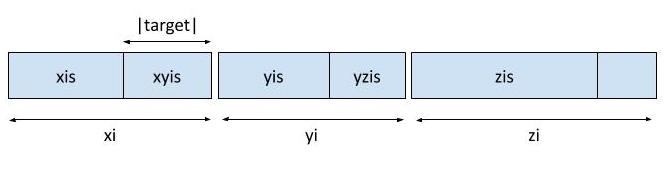
\includegraphics[scale=0.5]{text/stringmatcher/AssociativeIndices}
\caption{Associativity of String Matching.}
\label{fig:mappend:assoc}
\end{figure}
We now sketch the three proof steps, while the whole proof
is available online~\cite{implementation}.
\begin{code}
  assoc x@(SM xi xis) y@(SM yi yis) z@(SM zi zis)
    -- Step 1: unwrapping the indices
    =   x <> (y <> z)
    =. (SM xi xis) <> ((SM yi yis) <> (SM zi zis))
                         ...
    -- via list associativity and distribution of shifts
    =. SM i (xis1 ++ ((xyis1 ++ yis1 ++ yzis1) ++ zis1))
    -- Step 2: Equivalence of representations
    =. SM i (xis2 ++ ((xyis1 ++ yis1 ++ yzis1) ++ zis1))
       ? castConcat tg xi yi zi xis
    =. SM i (xis2 ++ ((xyis1 ++ yis1 ++ yzis1) ++ zis2))
       ? mapLenFusion tg xi yi zi zis
    =. SM i (xis2 ++ ((xyis2 ++ yis2 ++ yzis2) ++ zis2))
       ? assocNewIndices y tg xi yi zi yis
    -- Step 3: Wrapping the indices
                         ...
    -- via list associativity and distribution of casts
    =. (SM xi xis <> SM yi yis) <> SM zi zis
    =. (x <> y) <> z
    ** QED
    where
      i     = xi stringMappend (yi stringMappend zi)

      yzis1 = map (shiftStringRight tg xi (yi <+> zi)) yzis
      yzis2 = makeNewIndices (xi <+> yi) zi tg
      yzis  = makeNewIndices yi zi tg
      ...
\end{code}
\cqed\end{proof}


\subsection{String Matching Monoid Morphism}\label{subsec:smmorphism}
Next, we define the function @toSM :: RString -> SM target@ which does
the actual string matching computation for a set
target~\footnote{\texttt{toSM} assumes the target is clear from the
  calling context; it is also possible to write a wrapper function
  taking an explicit target which gets existentially reflected into
  the type.}
%
\ignore{ The function @toSM input@ creates a string matcher @SM
  target@ structure that matches the type level symbol target to the
  string value argument @input@.  }
%
\begin{code}
toSM :: forall (target :: Symbol). (KnownSymbol target)
     => RString -> SM target
toSM input = SM input (makeSMIndices input tg) where
  tg = fromString (symbolVal (Proxy :: Proxy target))

makeSMIndices
  :: x:RString -> tg:RString -> [GoodIndex x tg]
makeSMIndices x tg
  = makeIndices x tg 0 (lenStr tg - 1)
\end{code}
%
The input field of the result is the input string;
the indices field is computed by calling @makeIndices@
within the range of the @input@, that is from
@0@ to @lenStr input - 1@.
%
\begin{code}
\end{code}

We now prove that @toSM@ is a monoid morphism.
%
\begin{theorem}[$\texttt{toSM}$ is a Morphism]\label{theorem:smmorphism}
@toSM :: RString -> SM t@ is a morphism between the monoids
(@RString@, @stringMempty@, @stringMappend@) and (@SM t@, @mempty@, @mappend@).
\end{theorem}
\begin{proof}
Based on definition~\ref{definition:morphism}, proving @toSM@
is a morphism requires constructing a valid inhabitant of the type
\begin{code}
Morphism RString (SM t) toSM
  = x:RString -> y:RString
  -> {toSM stringMempty = mempty && toSM (x <+> y) = toSM x <> toSM y}
\end{code}
%
We define the function @distributestoSM :: Morphism RString (SM t) toSM@
to be the required valid inhabitant.

The core of the proof starts from
exploring the string matcher @toSM x <> toSM y@.
%
This string matcher contains three sets of indices
as illustrated in Figure~\ref{fig:mappend:indices}:
(1) @xis@ from the input @x@,
(2) @xyis@ from appending the two strings, and
(3) @yis@ from the input @y@.
%
We prove that appending these three groups of indices together gives
exactly the good indices of @x stringMappend y@, which are also the
value of the indices field in the result of
%
@toSM (x stringMappend y)@.
\begin{code}
distributestoSM x y
  =   (toSM x :: SM target) <> (toSM y :: SM target)
  ==. (SM x is1) <> (SM y is2)
  ==. SM i (xis ++ xyis ++ yis)
  ==. SM i (makeIndices i tg 0 hi1 ++ yis)
      ? (mapCastId tg x y is1 && mergeNewIndices tg x y)
  ==. SM i (makeIndices i tg 0       hi1
         ++ makeIndices i tg (hi1+1) hi)
      ? shiftIndicesRight 0 hi2 x y tg
  ==. SM i is
      ? mergeIndices i tg 0 hi1 hi
  ==. toSM (x <+> y)
  *** QED
  where
    xis  = map (castGoodIndexRight tg x y) is1
    xyis = makeNewIndices x y tg
    yis  = map (shiftStringRight   tg x y) is2
    tg   = fromString (symbolVal (Proxy::Proxy target))
    is1  = makeSMIndices x tg
    is2  = makeSMIndices y tg
    is   = makeSMIndices i tg
    i    = x <+> y
    hi1  = lenStr x - 1
    hi2  = lenStr y - 1
    hi   = lenStr i - 1
\end{code}
%
The most interesting lemma we use is
@mergeIndices x tg lo mid hi@
that states that for the input @x@ and the target @tg@
if we append the indices in the range  from @to@ to @mid@
with the indices in the range from @mid+1@ to @hi@,
we get exactly the indices in the range from @lo@ to @hi@.
%
This property is formalized in the type of the lemma.
\begin{code}
mergeIndices
 :: x:RString -> tg:RString
  -> lo:Nat -> mid:{Int | lo <= mid} -> hi:{Int | mid <= hi}
  -> {   makeIndices x tg lo hi
     =  makeIndices x tg lo mid
     ++ makeIndices x tg (mid+1) hi}
\end{code}
%
The proof proceeds by induction on @mid@ and using three more lemmata:
\begin{itemize}
\item @mergeNewIndices@ states that appending the indices @xis@ and @xyis@
is equivalent to the good indices of @x stringMappend y@ from @0@ to @lenStr x - 1@.
%
The proof case splits on the relative sizes of @tg@ and @x@
and is using @mergeIndices@ on @mid = lenStr x1 - lenStr tg@
in the case where @tg@ is smaller than @x@.
%
\item @mapCastId@ states that casting a list of indices returns the same list.
\item @shiftIndicesRight@ states that shifting right @i@ units the indices from @lo@ to @hi@
is equivalent to computing the indices from @i + lo@
to @i + hi@ on the string @x stringMappend y@, with @lenStr x = i@.
\end{itemize}
%%\begin{code}
%%mergeNewIndices
%%  :: tg:RString -> x:RString -> y:RString
%%  -> { makeSMIndices x tg
%%    ++ makeNewIndices x y tg
%%    == makeIndices (x <+> y) tg 0 (lenStr x - 1)}
%%\end{code}
%%The theorem states that appending the indices that appear in the first string @x@,
%%that is the indices @xis@ that do not and the indices @xyis@ that do involve @y@,
%%is equivalent to the indices @is@ on the input @x stringMappend y@
%%in the range from @0@ to @lenStr x -1@.
%%%
%%The proof case splits on the sizes of @tg@ and @x@.
%%%
%%If the size of the target is less than two, then @xyis@ is empty,
%%but @xis == is@, as appending @y@ to the input cannot create more indices.
%%%
%%Otherwise, if the input @x@ is smaller than the target,
%%then @xis@ is empty and @xyis@ is equal to @is@.
%%%
%%Otherwise, we set
%%and use the previous @mergeIndices@ lemma to merge @xis@ and @yis@ into @is@.
%%\item Shifting is left concatenation.
%%\begin{code}
%%shiftIndicesRight
%%  :: lo:Nat -> hi:Int
%%  -> x:RString -> y:RString
%%  -> tg:RString
%%  -> { map (shiftStringRight tg x y)
%%           (makeIndices y tg lo hi)
%%  == makeIndices (x stringMappend y) tg
%%                 (lenStr x + lo) (lenStr x + hi) }
%%
%%\end{code}
%%The lemma states that shifting indices from @lo@ to @hi@ on @y@
%%is equivalent to computing the indices from @lenStr x + lo@
%%to @lenStr x + hi@ on @x stringMappend y@,
%%and it is proved by induction on the difference @hi - lo@.
%%\end{itemize}
\qed\end{proof}


\subsection{Parallel String Matching}\label{subsec:parallel-string-matching}
We conclude this section with
the definition of a parallelized version of string matching.
%
We put all the theorems together to prove 
that the sequential and parallel versions always give the same result.
% and compare their time complexities.

We define @toSMPar@ as a parallel version of @toSM@ using machinery of section~\ref{sec:parallelization}.
\begin{code}
toSMPar :: forall (target :: Symbol). (KnownSymbol target)
        => Int -> Int -> RString -> SM target
toSMPar i j = pmconcat i . pmap toSM . chunkStr j
\end{code}
%
First, @chunkStr@ splits the input into @j@ chunks.
%
Then, @pmap@ applies @toSM@ at each chunk in parallel.
Finally, @pmconat@ concatenates the mapped chunks in parallel
using @mappend@, the monoidal operation for @SM target@.

\paragraph{Correctness.}
We prove correctness of @toSMPar@ directly from
Theorem~\ref{theorem:two-level}.
\begin{theorem}[Correctness of Parallel String Matching]\label{theorem:correctness}
For each parameter @i@ and @j@, and input @x@,
@toSMPar i j x@ is always equal to @toSM x@.
\begin{code}
correctness :: i:Int -> j:Int -> x:RString
             -> {toSM x = toSMPar i j x}
\end{code}
\end{theorem}

\begin{proof}
The proof follows by direct application of Theorem~\ref{theorem:two-level}
on the chunkable monoid (@RString@, @$\eta$@, @<+>@) (by Assumption~\ref{assumption:rstring})
and the monoid (@SM t@, @$\epsilon$@, @<>@) (by Theorem~\ref{theorem:stringmatchers}).
%
\begin{code}
correctness i j x
  =   toSMPar i j x
  ==. pmconcat i (pmap toSM (chunkStr j x))
  ==. toSM is
    ? parallelismEquivalence toSM distributestoSM x i j
  *** QED
\end{code}
%
Note that application of the theorem @parallelismEquivalence@
requires a proof that its first argument @toSM@ is a morphism.
%
By Theorem~\ref{theorem:monoid:distribution},
the required proof is provided as the function @distributestoSM@.
\qed\end{proof}

\ignore{

\paragraph{Time Complexity.}
Counting only string comparisons as the expensive operations,
the sequential string matcher on input @x@ runs in time
linear to @n = lenStr x@. Thus $T_\texttt{toSM}(n) = O(n)$.

We get time complexity of @toSMPar@ by the time complexity of
two-level parallel algorithms equation~\ref{eq:complexity},
with the time of string matching mappend being linear on the length
of the target @t = lenStr tg@, or
$T_\mappend(\texttt{SM})= O(t)$.
%
$$
T_\texttt{toSMPar} (n, t, i, j) =
O((i-1)(\frac{\log n - \log j}{\log i}) t  + \frac{n}{j})
$$
%
The above analysis refers to a model with infinite processor and no caching.
To compare the algorithms in practice,
we matched the target "the"
in  Oscar Wilde's "The Picture of Dorian Gray", a text of @n = 431372@ characters
using a two processor Intel Core i5.
%
The sequential algorithm detected 4590 indices in 40 ms.
%
We experimented with different parallization factors @i@ and chunk sizes @j / n@
and observed up to $50\%$ speedups of the parallel algorithm for parallelization factor
@4@ and @8@ chunks.
%
As a different experiment, we matched the input against its size @t = 400@ prefix,
a size comparable to the input size @n@.
%
For bigger targets,
mappend gets slower, as it has complexity linear to the size of target.
%
We observed $20\%$ speedups for @t=400@ target but also $30\%$ slow downs for various sizes of @i@ and @j@.
%
In all cases the indices returned by the sequential and the parallel algorithms were the same.
}


\section{Evaluation: Strengths \& Limitations}\label{sec:evaluation}

Verification of Parallel String Matching is the first realistic
proof that uses (Liquid) Haskell
to prove properties \textit{about} program functions.
%
In this section we use the String Matching proof
to quantitatively and qualitatively evaluate theorem proving in Haskell.

\paragraph{Quantitative Evaluation.}
The Correctness of Parallel String Matching proof
can be found online~\cite{implementation}.
%
Verification time, that is the time Liquid Haskell needs to check the proof,
is 75 sec on a dual-core Intel Core i5-4278U processor.
%
The proof consists of \textit{1839} lines of code.
%
Out of those
\begin{itemize}
\item \textit{226} are Haskell ``runtime'' code,
\item \textit{112} are liquid comments on the ``runtime'' Haskell code,
\item \textit{1307} are Haskell proof terms, that is functions with @Proof@ result type, and
\item \textit{194}  are liquid comments to specify theorems.
\end{itemize}
Counting both liquid comments and Haskell proof terms as verification code,
we conclude that the proof requires 7x the lines of ``runtime'' code.
%
This ratio is high and takes us to 2006 Coq,
when Leroy~\cite{Leroy06formalcertification} verified
the initial CompCert C compiler with
the ratio of verification to compiler lines being 6x.
% 4,400 lines of compiler code and 28,000 lines devoted to verification.

\paragraph{Strengths.}
Though currently verbose,
deep verification using Liquid Haskell has many benefits.
%
First and foremost,
\textit{the target code is written in the general purpose Haskell}
and thus can use advanced Haskell features, including
type literals, deriving instances, inline annotations
and optimized library functions like @ByteString@.
Even diverging functions can coexist with the target code, as long
as they are not reflected into logic~\cite{Vazou14}.

Moreover, \textit{SMTs are used to automate the proofs}
over key theories like linear arithmetic and equality.
%
As an example, associativity of @(+)@
is assumed throughout the proofs while shifting indices.
%
Our proof could be further automated 
by mapping refined strings to SMT strings and  
using the automated SMT string theory.
%
We did not follow this approach because we want to show that
our techinique can be used to prove any (and not only domain specific)
program properties.

Finally, we get further automation via
\textit{Liquid Type Inference}~\cite{LiquidPLDI08}.
%
Properties about program functions,
expressed as type specifications with unit result,
often depend on program invariants,
expressed as vanilla refinement types, and vice versa.
%
For example, we need the invariant that all indices of
a string matcher are good indices
to prove associativity of @(mappend)@.
%%NV simplify the above.
%%%For example, we need the invariant that all indices of
%%%a string matcher are good indices
%%%to prove that
%%%when the target is smaller than the input
%%%then the indices field is an empty list,
%%%which is required to prove associativity of @(mappend)@
%
Even though Liquid Haskell cannot currently synthesize proof terms,
it performs really well at inferring and propagating program invariants (like good indices)
via the abstract interpretation framework of Liquid Types.

\paragraph{Limitations.}
There are severe limitations that should be addressed
to make theorem proving in Haskell a pleasant and usable technique.
%
As mentioned earlier \textit{the proofs are verbose}.
%
There are a few cases where the proofs require domain specific knowledge.
%
For example, to prove associativity of string matching
@x mappend (y mappend z) = (x mappend y) mappend z@
we need a theorem that performs case analysis on the relative length of
the input field of @y@ and the target string.
%
Unlike this case split though, most proofs
do not require domain specific knowledge and merely proceed
by term rewriting and structural inductuction
that should be automated
via Coq-like~\cite{coq-book} tactics or/and Dafny-like~\cite{dafny} heuristics.
%
For example, synquid~\cite{polikarpova16} could be used to automatically
synthesize proof terms.

Currently, we suffer from two engineering limitations.
%
First, all reflected function should exist in the same module,
as reflection needs access to the function implementation
that is unknown for imported functions.
%
This is the reason why we need to use a user defined,
instead of Haskell's built-in, list.
%
In our implementation we used @CPP@ as a current workaround
of the one module restriction.
%
Second, class methods
cannot be currently reflected.
%
Our current workaround is to define Haskell functions instead
of class instances.
For example (@append@, @nil@) and (@concatStr@, @emptyStr@)
define the monoid methods of List and Refined String respectively.

Overall, we believe that the strengths outweigh the limitations which
will be addressed in the near future,
rendering Haskell a powerful theorem prover.

\section{Conclusion}\label{sec:conclusion}
We made the first non-trivial use of (Liquid) Haskell as a proof
assistant. 
We proved the parallelization of chunkable monoid
morphisms to be correct
and applied our parallelization technique to string matching,
resulting in a formally verified parallel string matcher.
%
Our proof uses refinement types to specify
equivalence theorems,
Haskell terms to express proofs,
and Liquid Haskell to check that the terms prove the theorems.
%
Based on our 1839LoC sophisticated proof we conclude that
Haskell can be successfully used as a theorem prover
to prove arbitrary theorems about real Haskell code
using SMT solvers to automate proofs
over key theories like linear arithmetic and equality.
%
However, Coq-like tactics or Dafny-like heurestics are required
to ease the user from manual proof term generation.


\begin{comment}
  - lines of code
  - interaction of proofs with code
        no interaction: the main proof
        invariant good indices are requied to prove that
           if target it bigger than input then indices is empty
           proof oof good indexing requires casting
   - proof reuse
   - trust library factions with assume annotations
\end{comment}


\mypara{Acknowledgments}
The material of this chapter have been submitted for publication as it may appear in ESOP 2017:
\noindent Vazou, Niki; Polakow, Jeff.
``Verified Parallel String Matching in Haskell''.